%%%%%%%%%%%%%%%%%%%%%%%%%%%%%%%%%%%%%%%%%
% This is a template for LaTeX thesis (M.Sc. or PhD) at ZHAW.
% 
% ZHAW thesis template downloaded from:
% https://github.com/matteodelucchi/ZHAW_thesis-template
% 
% University specific changes were made by:
% Matteo Delucchi
%
% Based on a template downloaded from:
% http://www.LaTeXTemplates.com
% 
% Version 2.x major modifications by:
% Vel (vel@latextemplates.com)
%
% This template is based on a template by:
% Steve Gunn (http://users.ecs.soton.ac.uk/srg/softwaretools/document/templates/)
% Sunil Patel (http://www.sunilpatel.co.uk/thesis-template/)
%
% Template license:
% CC BY-NC-SA 3.0 (http://creativecommons.org/licenses/by-nc-sa/3.0/)
%
%%%%%%%%%%%%%%%%%%%%%%%%%%%%%%%%%%%%%%%%%

%----------------------------------------------------------------------------------------
%	PACKAGES AND OTHER DOCUMENT CONFIGURATIONS
%----------------------------------------------------------------------------------------

\documentclass[
11pt, % The default document font size, options: 10pt, 11pt, 12pt
%oneside, % Two side (alternating margins) for binding by default, uncomment to switch to one side
english, % ngerman for German
singlespacing, % Single line spacing, alternatives: onehalfspacing or doublespacing
%draft, % Uncomment to enable draft mode (no pictures, no links, overfull hboxes indicated)
%nolistspacing, % If the document is onehalfspacing or doublespacing, uncomment this to set spacing in lists to single
%liststotoc, % Uncomment to add the list of figures/tables/etc to the table of contents
%toctotoc, % Uncomment to add the main table of contents to the table of contents
%parskip, % Uncomment to add space between paragraphs
%nohyperref, % Uncomment to not load the hyperref package
headsepline, % Uncomment to get a line under the header
%chapterinoneline, % Uncomment to place the chapter title next to the number on one line
%consistentlayout, % Uncomment to change the layout of the declaration, abstract and acknowledgements pages to match the default layout
]{MastersDoctoralThesis} % The class file specifying the document structure

\usepackage[utf8]{inputenc} % Required for inputting international characters
\usepackage[T1]{fontenc} % Output font encoding for international characters
\usepackage{xcolor}

%\usepackage[x-5pg]{pdfx} %for PDF-X support. Has problems with xcolor and hyperref
%\usepackage{subfigure}
\usepackage{caption}
\usepackage{subcaption}

\usepackage{mathpazo} % Use the Palatino font by default

\usepackage[backend=biber,  % Use the bibtex backend with the authoryear citation style (which resembles APA)
sorting=none, % numbers the reference in order of their appearance in the document. Troubleshoot with deleting all *.aux and *.bbl files and rebuild.
style=numeric-comp,
natbib=true]{biblatex}

\addbibresource{example.bib} % The filename of the bibliography

\usepackage[autostyle=true]{csquotes} % Required to generate language-dependent quotes in the bibliography

\usepackage{pdfpages}

\usepackage{todonotes}
\setlength{\marginparwidth}{2.5cm} % uncomment this if the todonotes are out of margins (cut off page)

\usepackage{listings}
\usepackage{physics}
\usepackage{minted}
\usepackage[braket, qm]{qcircuit}
\usepackage{graphicx}

\usepackage{tikz}
\usetikzlibrary{positioning}

\definecolor{codegreen}{rgb}{0,0.6,0}
\definecolor{codegray}{rgb}{0.5,0.5,0.5}
\definecolor{codepurple}{rgb}{0.58,0,0.82}
\definecolor{backcolour}{rgb}{0.921, 0.929, 0.937} %0.95,0.95,0.92

\lstdefinestyle{mystyle}{
backgroundcolor=\color{backcolour},   
commentstyle=\color{codegreen},
keywordstyle=\color{magenta},
numberstyle=\tiny\color{codegray},
stringstyle=\color{codepurple},
basicstyle=\ttfamily\footnotesize,
breakatwhitespace=false,         
breaklines=true,                 
captionpos=b,                    
keepspaces=true,                 
numbers=left,                    
numbersep=5pt,                  
showspaces=false,                
showstringspaces=false,
showtabs=false,                  
tabsize=2
}

\lstset{style=mystyle}

\usepackage{makecell} % formatting tables

%needed to display svgs
\usepackage{svg}



%----------------------------------------------------------------------------------------
%	MARGIN SETTINGS
%----------------------------------------------------------------------------------------

\geometry{
paper=a4paper, % Change to letterpaper for US letter
inner=2.5cm, % Inner margin
outer=3.8cm, % Outer margin
bindingoffset=.5cm, % Binding offset
top=1.5cm, % Top margin
bottom=1.5cm, % Bottom margin
%showframe, % Uncomment to show how the type block is set on the page
}


%----------------------------------------------------------------------------------------
%	THESIS INFORMATION
%----------------------------------------------------------------------------------------

\thesistitle{Implementing Neural Networks In A Quantum Computer} % Your thesis title, this is used in the title and abstract, print it elsewhere with \ttitle
\supervisor{Prof. Dr. Kurt \textsc{Stockinger} \\ Prof. Dr. Rudolf Marcel \textsc{Füchslin}} % Your supervisor's name, this is used in the title page, print it elsewhere with \supname
\examiner{} % Your examiner's name, this is not currently used anywhere in the template, print it elsewhere with \examname
\degree{Research Project} % Your degree name (Doctor of Philosophy or Master of Science), this is used in the title page and abstract, print it elsewhere with \degreename
\author{Ricardo Daniel \textsc{Monteiro Simões},  Patrick \textsc{Huber}}
\addresses{} % Your address, this is not currently used anywhere in the template, print it elsewhere with \addressname

\keywords{} % Keywords for your thesis, this is not currently used anywhere in the template, print it elsewhere with \keywordnames
\university{\href{https://www.zhaw.ch/en/university/}{Zurich University of Applied Sciences}} % Your university's name and URL, this is used in the title page and abstract, print it elsewhere with \univname
\universitygerman{\href{https://www.zhaw.ch/de/hochschule/}{Z{\"u}rcher Hochschule f{\"u}r Angewandte Wissenschaften}}% Your university's name in german and URL, this is used in the german abstract (Zusammenfassung), print it elsewhere with \univnameger
\department{\href{https://www.zhaw.ch/de/engineering/institute-zentren/init/}{Institute of Applied Information Technology}} % Your department's name and URL, this is used in the title page and abstract, print it elsewhere with \deptname
\group{\href{https://www.zhaw.ch/de/engineering/institute-zentren/init/}{Institut für angewandte Informationstechnologie}} % Your research group's name and URL, this is used in the title page, print it elsewhere with \groupname
\faculty{\href{https://www.zhaw.ch/de/lsfm/}{Life Sciences and Facility Management}} % Your faculty's name and URL, this is used in the title page and abstract, print it elsewhere with \facname

\AtBeginDocument{
\hypersetup{pdftitle=\ttitle} % Set the PDF's title to your title
\hypersetup{pdfauthor=\authorname} % Set the PDF's author to your name
\hypersetup{pdfkeywords=\keywordnames} % Set the PDF's keywords to your keywords
}

\begin{document}

\frontmatter % Use roman page numbering style (i, ii, iii, iv...) for the pre-content pages

\pagestyle{plain} % Default to the plain heading style until the thesis style is called for the body content

%----------------------------------------------------------------------------------------
%	TITLE PAGE
%----------------------------------------------------------------------------------------

\begin{titlepage}
\begin{center}

\begin{figure}
\centering

\includegraphics[width=0.15\textwidth]{Figures/ZHAW_Logo.png} % Universtiy Logo, Adapted from: https://upload.wikimedia.org/wikipedia/commons/thumb/e/e6/ZHAW_Logo.svg/879px-ZHAW_Logo.svg.png
\end{figure}

\vspace*{.06\textheight}
{\scshape\LARGE \univname\par}\vspace{1.5cm} % University name
\textsc{\Large Research Project}\\[0.5cm] % Thesis type

\HRule \\[0.4cm] % Horizontal line
{\huge \bfseries \ttitle\par}\vspace{0.4cm} % Thesis title
\HRule \\[1.5cm] % Horizontal line
 
\begin{minipage}[t]{0.4\textwidth}
\begin{flushleft} \large
\emph{Authors:}\\
\authorname % Author name - remove the \href bracket to remove the link
\end{flushleft}
\end{minipage}
\begin{minipage}[t]{0.4\textwidth}
\begin{flushright} \large
\emph{Supervisors:} \\
\supname % Supervisor name - remove the \href bracket to remove the link  
\end{flushright}
\end{minipage}\\[3cm]
 
\vfill

%\large \textit{A project thesis submitted in fulfillment of the requirements}\\[0.3cm] % University requirement text
%\textit{of the}\\[0.4cm]
%\groupname\\
%\deptname\\[2cm] % Research group name and department name
 
\vfill

{\large \today}\\[4cm] % Date
%\includegraphics{Logo} % University/department logo - uncomment to place it
 
\vfill
\end{center}
\end{titlepage}

%----------------------------------------------------------------------------------------
%	DECLARATION PAGE
%----------------------------------------------------------------------------------------

\begin{declaration}
\addchaptertocentry{\authorshipname} % Add the declaration to the table of contents

\noindent We, \authorname, declare that this research project thesis titled, \enquote{\ttitle} and the work presented in it are of our own. We confirm that:

\begin{itemize} 
\item Where I have consulted the published work of others, this is always clearly attributed.
\item Where I have quoted from the work of others, the source is always given. With the exception of such quotations, this thesis is entirely my own work.
\item I have acknowledged all main sources of help.
\item Where the thesis is based on work done by ourselves jointly with others, we have made clear exactly what was done by others and what we have contributed ourselves.\\
\end{itemize}
 
\noindent Signed:\\
\rule[0.5em]{25em}{0.5pt} % This prints a line for the signature

\noindent Signed:\\
\rule[0.5em]{25em}{0.5pt} % This prints a line for the signature

\noindent Date:\\
\rule[0.5em]{25em}{0.5pt} % This prints a line to write the date
\end{declaration}

\cleardoublepage

%----------------------------------------------------------------------------------------
%	QUOTATION PAGE
%----------------------------------------------------------------------------------------

%\vspace*{0.2\textheight}

% \noindent\enquote{\itshape I'm fascinated by the idea that genetics is digital. A gene is a long sequence of coded letters, like computer information. Modern biology is becoming very much a branch of information technology.}\bigbreak

% \hfill Richard Dawkins


% \vspace*{0.2\textheight}

% \noindent\enquote{\itshape A line is a dot that went for a walk.}\bigbreak

% \hfill Paul Klee
%\todo{find a good quote}
%\noindent\enquote{\itshape You can’t connect the dots looking forward; you can only connect them looking backwards. So you have to trust that the dots will somehow connect in your future. You have to trust in something – your gut, destiny, life, karma, %whatever. Because believing that the dots will connect down the road will give you the confidence to follow your heart even when it leads you off the well worn path; and that will make all the difference.
%}\bigbreak
%\hfill{Steve Jobs} \newline 
%\strut\hfill{\tiny{(Stanford commencement speech, June 2005)}}

%----------------------------------------------------------------------------------------
%	ABSTRACT PAGE
%----------------------------------------------------------------------------------------

\begin{abstract}
\addchaptertocentry{\abstractname} % Add the abstract to the table of contents
One important part of neural networks are computational neurons and their highly adapted derivatives. This has allowed neural networks to offer solutions to otherwise hard to solve problems. Theoretical expectations and current advancements in the field of quantum computation allow us to develop and evaluate neuron designs that are self contained, quantum circuits. We show through various experiments and observations that whilst the classical neuron can be recreated, it sorely lacks usage of any features that make the field of quantum computation powerful. We propose a new design for quantum neurons that can be adapted on any $x$ features and $y$ classes classification problem, with acceptable results, but also show that the current route of gradient-based optimization for quantum circuits offered through IBMs qiskit has its own pitfalls.
\end{abstract}

%----------------------------------------------------------------------------------------
%	German ABSTRACT PAGE
%----------------------------------------------------------------------------------------

%\begin{extraAbstract}
%    \addchaptertocentry{\extraabstractname} % Add the abstract to the table of contents
%Die Zusammenfassung der Dissertation wird hier geschrieben (und normalerweise nur auf dieser Seite gehalten). Die Seite wird %vertikal zentriert, so dass sie sich auch in den leeren Raum über dem Titel ausdehnen kann\ldots
%
%Strukturiere sie wie folgt: Kontext, Bedarf (was wir haben), Bedarf (was wir wollen), Aufgabe, Gegenstand des Dokuments, %Ergebnisse, Schlussfolgerung und Perspektiven. 
%    
%\end{extraAbstract}
%----------------------------------------------------------------------------------------
%	ACKNOWLEDGEMENTS
%----------------------------------------------------------------------------------------

%\begin{acknowledgements}
%\addchaptertocentry{\acknowledgementname} % Add the acknowledgements to the table of contents
%The acknowledgments and the people to thank go here, don't forget to include your project advisor\ldots
%\end{acknowledgements}

%----------------------------------------------------------------------------------------
%	LIST OF CONTENTS
%----------------------------------------------------------------------------------------

\tableofcontents % Prints the main table of contents

%----------------------------------------------------------------------------------------
%	DEDICATION
%----------------------------------------------------------------------------------------

%\dedicatory{For/Dedicated to/To my\ldots} 

%----------------------------------------------------------------------------------------
%	PREFACE
%----------------------------------------------------------------------------------------

%\begin{preface}
%   \addchaptertocentry{\prefacename} % Add the acknowledgements to the table of contents
%   Explain the motivation for the topic in general. Go through each chapter and explain how they contribute to your research %question.
%    Check the thesis of Johannes John Carel Kuiper for a good example preface: %\url{https://dspace.library.uu.nl/bitstream/handle/1874/90/full.pdf?sequence=2&isAllowed=y}
%\end{preface}

%----------------------------------------------------------------------------------------
%	THESIS CONTENT - CHAPTERS
%----------------------------------------------------------------------------------------

\mainmatter % Begin numeric (1,2,3...) page numbering

\pagestyle{thesis} % Return the page headers back to the "thesis" style

% Include the chapters of the thesis as separate files from the Chapters folder
% Uncomment the lines as you write the chapters

% Chapter 6

\chapter{Introduction} % Main chapter title

\label{chapter:introduction}

The ever occurring question \emph{"Can quantum $x$ beat the classical variant?"} was once a synonym for \emph{theoretically, yes}. For a long time all possible gains remained in the theoretical realm\cite{shor_polynomial-time_1997}, but current advances in the field of quantum computing have brought out solutions and proposals\cite{farhi_quantum_2014, fankhauser_multiple_2021, havlicek_supervised_2019} that can be programmed and used \emph{today}. At the same time quantum computing is getting more and more available to non-researchers as IBM, Microsoft, Google and co. fight for dominance in this new field of computation.\par
The training of neural networks demands an ever increasing amount of computational power\cite{openai_ai_2018} to train algorithms that can solve the worlds hardest problems. The goal of this paper is to evaluate current quantum offerings to solve classification problems as well as analyse their performance. In a first step, the application of features and weights onto a quantum gates and their behaviour is assessed. Subsequently two possible designs are evaluated. The first solution replicates the basic arithmetic operations computational neurons use, and the second one uses quantum specific superpositions and entanglement. Due to the necessary amount of qubits for the arithmetic solution, as well as the absence of quantum specific operations, only the the classifier based on entanglement and superpositions is further developed and evaluated.\par 
Using a variety of different quantum circuits, as well as three different datasets, training is done on the simulator to determine the viability of these designs as well as to compare them to a basic \code{MLP} classifier. The results show that the right combination of quantum gates leads to a more flexible classifier, that can adapt and solve different problem spaces. One problem that accompanies these design is the disparity when it comes to achieved accuracy. Under reproducible circumstances, no two training results are equal. This problem comes directly from the vast expressability such a circuit offers - by making the problem space much wider, it gets harder to traverse and therefor, find a viable solution.\par 
When running the trained circuit on real hardware for a given dataset, another problem arises as the noise affecting a real devices disrupts the operations and leads to vastly inferior accuracy. As current The findings show that quantum circuits can offer a substantial gain when compared to the classical solutions, but still need more refinement before being touted as a viable alternative, without regards to hardware availability. 
\chapter{Computational Neuron} % Chapter title

\label{chapter:computational_neuron} % For referencing the chapter elsewhere, use \ref{chapter:computational_neuro} 

%----------------------------------------------------------------------------------------

% Define some commands to keep the formatting separated from the content 
\newcommand{\keyword}[1]{\textbf{#1}}
\newcommand{\tabhead}[1]{\textbf{#1}}
\newcommand{\code}[1]{\texttt{#1}}
\newcommand{\file}[1]{\texttt{\bfseries#1}}
\newcommand{\option}[1]{\texttt{\itshape#1}}

%----------------------------------------------------------------------------------------

\section{Classical Variant}
The classic computational neuron, often referred to as perceptron, is a multi-step process that amounts to a single result that can be used in further neurons, or directly read out as an output. In their simplest form, the neuron has $n$ input features that are multiplied with $n$ weights. In addition to those features, there is a weighted bias, where the feature itself has the fixed value $1$. These values are then summarized and evaluated through an activation function $f(x)$. Originally proposed by Rosenblatt F.\cite{rosenblatt_perceptron_1958}, the structure of neuron with $n = 4$ input features and one bias feature is shown in figure \ref{figure:computation_neuron}\footnote{There are many iterations of this design that range from a different handling of the bias to multiple output designs like LSTMs\cite{lstm}}. A more formal definition is presented in equation \ref{equation:computation_neuron}, where $j=0$ is the bias.

\begin{figure}[h!]
    \centering
    \begin{tikzpicture}[shorten >=1pt,node distance=1.5cm,on grid,auto]
    	\node (0) {$i_0$};
    	\node (1) [below=of 0] {$i_1$};
    	\node (2) [below=of 1] {$i_2$};
    	\node (3) [below=of 2] {$i_3$};
    	\node (4) [below=of 3] {$i_4$};
    	\node (5) [right=of 2] {$\Sigma$};
    	\node (6) [right=of 5] {$f(x)$};
    	\node (7) [right=of 6] {$y$};
    	\path[->]
    	(0) edge [bend left=45] node {$\omega_0$} (5)
    	(1) edge [bend left=25] node {$\omega_1$} (5)
    	(2) edge  node {$\omega_2$} (5)
    	(3) edge [bend right=25] node {$\omega_3$} (5)
    	(4) edge [bend right=45] node {$\omega_4$} (5)
    	(5) edge node {} (6)
    	(6) edge node {} (7);
    \end{tikzpicture}
    \caption{Computational neuron with 4 features and 1 bias}
    \label{figure:computation_neuron}
\end{figure}

\begin{equation}
    \centering
    y =\ f\left(\sum_{j = 0}^n i_j\omega_j\right)
    \label{equation:computation_neuron}
\end{equation}

\newpage

The activation function $f(x)$, also called transfer function, can be selected from a plethora of valid choices\cite{szandala_review_2021}, depending on the problem at hand. Dissecting the neuron leads to the two key components needed for the creation of an equivalent quantum neuron: A function for addition $U_{+}$ and one for multiplication $U_{\times}$ (The activation function can then be constructed from these). Whilst a single qubit can be in a coherent superposition of two different states\cite{nielsen_quantum_2010}, its measurements always amount to either 0 or 1, with their respective probabilities. Due to this the implementation uses binary data input. The implementation also neglects the usage of \emph{entanglement} and \emph{superpositions} as the arithmetic functions do not make usage of probabilistic calculations.

%------------------------------------------------------------------------------------------
\section{Binary Addition}\label{chapter:binary_addition}

Binary addition allows the combination of all components $i_j\omega_j$ into a single variable $x$ used in the summation. It is also a prerequisite to creating the binary multiplication circuit. The rules that define binary addition are relatively simple and are summarized in table \ref{table:binary_addition_rules} for the expression $x_A + x_B =\ y$\\
\begin{table}[!h]
\centering
\begin{tabular}{|c|c|c|c|}
\hline
$x_A$ & $x_B$ & $y$ \\ \hline
0    & 0    & 0  \\ \hline
0    & 1    & 1  \\ \hline
1    & 0    & 1  \\ \hline
1    & 1    & 0  \\ \hline
\end{tabular}
\caption{Binary addition of two $1$ bit wide words}
\label{table:binary_addition_rules}
\end{table}

With table \ref{table:binary_addition_rules} a matrix $U_{+}$ can be created, that follows the given rules that apply to the creation of quantum gates\cite{scherer_quantum_2019}. Simply speaking, the matrix has to fulfill $U_{+}U_{+}^\dagger = I$. This is also often referred to as \emph{bijective} when working with functions. It dictates that any single resulting state can be followed back to a single input state. To fulfill these prerequisites, we have to use 3 qubits to assert no loss of information. The first two qubits are input bits $x_A$ and $x_B$, respectively, whilst the third one is output bit $y$. In this case, the vector $\vec{S}$ stands for any of the $2^3 = 8$ possible \emph{measurement} states the 3 qubits can be in, and vector $\vec{O}$ to any possible output state, as shown in equation \ref{equation:basic_quantum_calculation}.\\

\begin{equation}
    U_{+}\vec{S} = \vec{O} \rightarrow U_{+} =\ OS^T
    \label{equation:basic_quantum_calculation}
\end{equation}

First we create the state matrix $S$ that represents all possible input states of our quantum circuit.

\begin{equation}
    \begin{split}
        \vec{S_0} =\ \ket{0} \otimes \ket{0} \otimes \ket{0} &=\ \begin{pmatrix} 1 \\ 0\end{pmatrix}\ \otimes \begin{pmatrix}1 \\ 0\end{pmatrix} \otimes \begin{pmatrix}1 \\ 0\end{pmatrix} =\ \begin{pmatrix}1 \\0 \\0 \\0 \\0 \\0 \\0 \\0 \end{pmatrix}\\
        \rightarrow S &= I^{8\times8}
    \end{split}
    \label{equation:state_matrix_is_identity_matrix}
\end{equation}

Using the same method and the information from table \ref{table:binary_addition_rules} we construct the output state matrix $O$ in equation \ref{equation:addition_output_matrix}.

\begin{equation}
    \begin{split}
        \text{1. Row:}\ x_{A} + x_{B} = y \rightarrow \ket{0} + \ket{0} = \ket{0}\\    
        \text{2. Row:}\ x_{A} + x_{B} = y \rightarrow \ket{0} + \ket{1} = \ket{1}\\    
        \text{3. Row:}\ x_{A} + x_{B} = y \rightarrow \ket{1} + \ket{0} = \ket{1}\\    
        \text{4. Row:}\ x_{A} + x_{B} = y \rightarrow \ket{1} + \ket{1} = \ket{0}\\    
    \end{split}
\end{equation}

\begin{equation}
\centering
    \begin{split}
        \vec{O}_0 &=\ \ket{0} \otimes \ket{0} \otimes \ket{0} =\ \begin{pmatrix}1 \\0 \\0 \\0 \\0 \\0 \\0 \\0 \end{pmatrix} \\
        \rightarrow O &=\ \begin{pmatrix}
        1 & 0 & 0 & 0 & 0 & 0 & 0 & 0\\
        0 & 0 & 0 & 0 & 0 & 1 & 0 & 0\\
        0 & 0 & 0 & 0 & 0 & 0 & 1 & 0\\
        0 & 0 & 0 & 1 & 0 & 0 & 0 & 0\\
        0 & 0 & 0 & 0 & 1 & 0 & 0 & 0\\
        0 & 1 & 0 & 0 & 0 & 0 & 0 & 0\\
        0 & 0 & 1 & 0 & 0 & 0 & 0 & 0\\
        0 & 0 & 0 & 0 & 0 & 0 & 0 &1
        \end{pmatrix}
    \end{split}
    \label{equation:addition_output_matrix}
\end{equation}

Note that the matrix $O$ in equation \ref{equation:addition_output_matrix} can be flipped, depending on what qubit is selected as output. The two matrices $O$ and $S$ can now be inserted into the equation $U_{+} = OS^T$ and solved for $U_{+}$, as per equation \ref{equation:addition_matrix_solved}

\begin{equation}
    \begin{split}
        U_{+} =\ OS^T &=\ \begin{pmatrix}
        1 & 0 & 0 & 0 & 0 & 0 & 0 & 0\\
        0 & 0 & 0 & 0 & 0 & 1 & 0 & 0\\
        0 & 0 & 0 & 0 & 0 & 0 & 1 & 0\\
        0 & 0 & 0 & 1 & 0 & 0 & 0 & 0\\
        0 & 0 & 0 & 0 & 1 & 0 & 0 & 0\\
        0 & 1 & 0 & 0 & 0 & 0 & 0 & 0\\
        0 & 0 & 1 & 0 & 0 & 0 & 0 & 0\\
        0 & 0 & 0 & 0 & 0 & 0 & 0 &1
        \end{pmatrix}\begin{pmatrix}
         1 & 0 & 0 & 0 & 0 & 0 & 0 & 0\\
         0 & 1 & 0 & 0 & 0 & 0 & 0 & 0\\ 
         0 & 0 & 1 & 0 & 0 & 0 & 0 & 0\\
         0 & 0 & 0 & 1 & 0 & 0 & 0 & 0\\
         0 & 0 & 0 & 0 & 1 & 0 & 0 & 0\\
         0 & 0 & 0 & 0 & 0 & 1 & 0 & 0\\
         0 & 0 & 0 & 0 & 0 & 0 & 1 & 0\\
         0 & 0 & 0 & 0 & 0 & 0 & 0 & 1\\
        \end{pmatrix} \\ 
        \rightarrow U_{+} &=\ \begin{pmatrix}
        1 & 0 & 0 & 0 & 0 & 0 & 0 & 0\\
        0 & 0 & 0 & 0 & 0 & 1 & 0 & 0\\
        0 & 0 & 0 & 0 & 0 & 0 & 1 & 0\\
        0 & 0 & 0 & 1 & 0 & 0 & 0 & 0\\
        0 & 0 & 0 & 0 & 1 & 0 & 0 & 0\\
        0 & 1 & 0 & 0 & 0 & 0 & 0 & 0\\
        0 & 0 & 1 & 0 & 0 & 0 & 0 & 0\\
        0 & 0 & 0 & 0 & 0 & 0 & 0 &1
        \end{pmatrix}
    \end{split}
    \label{equation:addition_matrix_solved}
\end{equation}
\newpage

Using IBMs \code{qiskit} the calculated matrix $U_{+}$ is turned into a quantum gate.

\begin{minted}{python}
from qiskit import QuantumCircuit
import qiskit.quantum_info as qi

n_qubits = 3

#Create the Gate
addition = qi.Operator([[1, 0, 0, 0, 0, 0, 0, 0],
                        [0, 0, 0, 0, 0, 1, 0, 0],
                        [0, 0, 0, 0, 0, 0, 1, 0],
                        [0, 0, 0, 1, 0, 0, 0, 0],
                        [0, 0, 0, 0, 1, 0, 0, 0],
                        [0, 1, 0, 0, 0, 0, 0, 0],
                        [0, 0, 1, 0, 0, 0, 0, 0],
                        [0, 0, 0, 0, 0, 0, 0, 1]])
\end{minted}

Binary addition that allows for bit words longer than one use a carry bit, which is then used as the input for the next addition. As the carry over is not always needed, we will use a separate quantum gate to calculate it. The rules for binary addition with carry over are listed in table \ref{table:binary_addition_carry_over}

\begin{table}[!h]
    \centering
    \begin{tabular}{|c|c|c|c|c|}
        \hline
        $carry_{in}$ & $x_A$ & $x_B$ & $y$ & $carry_{out}$ \\ \hline
        0             & 0     & 0     & 0   & 0              \\ \hline
        1             & 0     & 0     & 1   & 0              \\ \hline
        0             & 0     & 1     & 1   & 0              \\ \hline
        1             & 0     & 1     & 0   & 1              \\ \hline
        0             & 1     & 0     & 1   & 0              \\ \hline
        1             & 1     & 0     & 0   & 1              \\ \hline
        0             & 1     & 1     & 0   & 1              \\ \hline
        1             & 1     & 1     & 1   & 1              \\ \hline
        \end{tabular}
    \caption{Binary addition with carry over}
    \label{table:binary_addition_carry_over}
\end{table}

\newpage


As part $x_A + x_B = y$ is solved, only a solution for the $carry_{out}$ is created. It is important to note here that the $carry_{in}$ bit from table \ref{table:binary_addition_carry_over} is being reused as output bit $y$. Using the \emph{Toffoli Gate}, also called \code{CCNOT}\cite{qiskit_ccxgate_nodate}, we can use two controlling qubits to invert the state of a third one as demonstrated with figure \ref{fig:carry_over_circuit}.

\begin{figure}[!h]
    \centering
    \scalebox{1.0}{
        \Qcircuit @C=1.0em @R=0.8em @!R {
            \nghost{ {q}_{0} :  } & \lstick{ x_{A} :  } & \ctrl{1} & \qw & \ctrl{2} & \qw & \qw\\
            \nghost{ {q}_{1} :  } & \lstick{ x_{B} :  } & \ctrl{2} & \ctrl{1} & \qw & \qw & \qw\\
            \nghost{ {q}_{2} :  } & \lstick{ carry_{in}/y :      } & \qw & \ctrl{1} & \ctrl{1} & \qw & \qw\\
            \nghost{ {q}_{3} :  } & \lstick{ carry_{out} :  } & \targ & \targ & \targ & \qw & \qw\\ 
        }
    }
    \caption{Quantum circuit to calculate the carry over bit}
    \label{fig:carry_over_circuit}
\end{figure}

Combining these two solutions, we construct a quantum circuit to add any $n$ bit wide words together. Figure \ref{figure:four_bit_full_adder} demonstrates a circuit for the addition of two $4$ bit wide words\footnote{Note that we have replaced the X gates used previously to set the initial state with parameterized RX gates, where any variable that is $z = \pi$ leads to $\ket{1}$ and $z = 0$ to $\ket{0}$}.

\begin{figure}[!h]
    \centering
    \scalebox{0.5}{
    \Qcircuit @C=1.0em @R=0.2em @!R { \\
        \ghost{ {q}_{0} :  } & \lstick{ x_{A0} :  } & \gate{\mathrm{R_X}\,(\mathrm{a{\ensuremath{\theta}}})} \barrier[0em]{12} & \qw & \multigate{3}{\mathrm{carry\,over}}_<<<{0} & \multigate{2}{\mathrm{addition}}_<<<{0} & \qw & \qw & \qw & \qw & \qw & \qw & \qw & \qw & \qw\\ 
        \ghost{ {q}_{1} :  } & \lstick{ x_{B0} :  } & \gate{\mathrm{R_X}\,(\mathrm{b{\ensuremath{\theta}}})} & \qw & \ghost{\mathrm{carry\,over}}_<<<{1} & \ghost{\mathrm{addition}}_<<<{1} & \qw & \qw & \qw & \qw & \qw & \qw & \qw & \qw & \qw\\ 
        \ghost{ {q}_{2} :  } & \lstick{ y_{0} :  } & \qw & \qw & \ghost{\mathrm{carry\,over}}_<<<{2} & \ghost{\mathrm{addition}}_<<<{2} & \meter & \qw & \qw & \qw & \qw & \qw & \qw & \qw & \qw\\ 
        \ghost{ {q}_{3} :  } & \lstick{ carry_0 :  } & \qw & \qw & \ghost{\mathrm{carry\,over}}_<<<{3} & \multigate{3}{\mathrm{carry\,over}}_<<<{2} & \qw & \multigate{2}{\mathrm{addition}}_<<<{2} & \meter & \qw & \qw & \qw & \qw & \qw & \qw\\ 
        \ghost{ {q}_{4} :  } & \lstick{ x_{A1} :  } & \gate{\mathrm{R_X}\,(\mathrm{c{\ensuremath{\theta}}})} & \qw & \qw & \ghost{\mathrm{carry\,over}}_<<<{0} & \qw & \ghost{\mathrm{addition}}_<<<{0} & \qw & \qw & \qw & \qw & \qw & \qw & \qw\\ 
        \ghost{ {q}_{5} :  } & \lstick{ x_{B1} :  } & \gate{\mathrm{R_X}\,(\mathrm{d{\ensuremath{\theta}}})} & \qw & \qw & \ghost{\mathrm{carry\,over}}_<<<{1} & \qw & \ghost{\mathrm{addition}}_<<<{1} & \qw & \qw & \qw & \qw & \qw & \qw & \qw\\ 
        \ghost{ {q}_{6} :  } & \lstick{ carry_1 :  } & \qw & \qw & \qw & \ghost{\mathrm{carry\,over}}_<<<{3} & \qw & \multigate{3}{\mathrm{carry\,over}}_<<<{2} & \qw & \multigate{2}{\mathrm{addition}}_<<<{2} & \meter & \qw & \qw & \qw & \qw\\ 
        \ghost{ {q}_{7} :  } & \lstick{ x_{A2} :  } & \gate{\mathrm{R_X}\,(\mathrm{e{\ensuremath{\theta}}})} & \qw & \qw & \qw & \qw & \ghost{\mathrm{carry\,over}}_<<<{0} & \qw & \ghost{\mathrm{addition}}_<<<{0} & \qw & \qw & \qw & \qw & \qw\\ 
        \ghost{ {q}_{8} :  } & \lstick{ x_{B2} :  } & \gate{\mathrm{R_X}\,(\mathrm{f{\ensuremath{\theta}}})} & \qw & \qw & \qw & \qw & \ghost{\mathrm{carry\,over}}_<<<{1} & \qw & \ghost{\mathrm{addition}}_<<<{1} & \qw & \qw & \qw & \qw & \qw\\ 
        \ghost{ {q}_{9} :  } & \lstick{ carry_2 :  } & \qw & \qw & \qw & \qw & \qw & \ghost{\mathrm{carry\,over}}_<<<{3} & \qw & \multigate{3}{\mathrm{carry\,over}}_<<<{2} & \qw & \multigate{2}{\mathrm{addition}}_<<<{2} & \meter & \qw & \qw\\ 
        \ghost{ {q}_{10} :  } & \lstick{ x_{A3} :  } & \gate{\mathrm{R_X}\,(\mathrm{g{\ensuremath{\theta}}})} & \qw & \qw & \qw & \qw & \qw & \qw & \ghost{\mathrm{carry\,over}}_<<<{0} & \qw & \ghost{\mathrm{addition}}_<<<{0} & \qw & \qw & \qw\\ 
        \ghost{ {q}_{11} :  } & \lstick{ x_{B3} :  } & \gate{\mathrm{R_X}\,(\mathrm{h{\ensuremath{\theta}}})} & \qw & \qw & \qw & \qw & \qw & \qw & \ghost{\mathrm{carry\,over}}_<<<{1} & \qw & \ghost{\mathrm{addition}}_<<<{1} & \qw & \qw & \qw\\ 
        \ghost{ {q}_{12} :  } & \lstick{ carry_3 :  } & \qw & \qw & \qw & \qw & \qw & \qw & \qw & \ghost{\mathrm{carry\,over}}_<<<{3} & \qw & \qw & \qw & \qw & \qw\\ 
        \ghost{c:} & \lstick{c:} & \lstick{/_{_{4}}} \cw & \cw & \cw & \cw & \dstick{_{_{0}}} \cw \cwx[-11] & \cw & \dstick{_{_{1}}} \cw \cwx[-10] & \cw & \dstick{_{_{2}}} \cw \cwx[-7] & \cw & \dstick{_{_{3}}} \cw \cwx[-4] & \cw & \cw\\ 
        }
    }
    \caption{$4$ bit wide full adder\todo{add more explanation to image}}
    \label{figure:four_bit_full_adder}
\end{figure}

In figure \ref{figure:four_bit_full_adder} the $i$ in $x_{Ai}$ and $x_{Bi}$ stands for the $i$th bit in the word, starting with the LSB\footnote{Least significant bit}. Both the \emph{carry over} and \emph{addition} gates are the previously discussed ones. The numbering on their input side resembles the mapping of the incoming qubit to the \emph{internal qubit}. The figure also illustrates how the $carry_i$ qubit is reused as output qubit of the next addition step.

%----------------------------------------------------------------------------------------
\newpage

\section{Binary multiplication}
\label{chapter:binary_multiplication}

Using the same steps as in chapter \ref{chapter:binary_addition}, table \ref{table:binary_multiplication_rules} illustrates the binary multiplication rules.

\begin{table}[!h]
\centering
\begin{tabular}{|l|l|l|}
\hline
$x_A$ & $x_B$ & $y$ \\ \hline
0     & 0     & 0   \\ \hline
0     & 1     & 0   \\ \hline
1     & 0     & 0   \\ \hline
1     & 1     & 1   \\ \hline
\end{tabular}
\caption{Binary multiplication rules}
\label{table:binary_multiplication_rules}
\end{table}

The defined rules resemble only a subset of what makes binary multiplication work. The results of the multiplication get shifted one by one and then summarized. Figure \ref{figure:binary_multiplication_example} illustrates the procedure with a basic example.

\begin{figure}[!h]
\centering
\begin{tabular}{clllccllll}
$x_A$                   &  &   &   & 1                     & 0                     & 1 & 1 & 0 & 1 \\
$x_B$                   &  &   &   &                       &                       &   & 1 & 0 & 1 \\ \hline
                        &  &   &   & 1                     & 0                     & 1 & 1 & 0 & 1 \\
                        &  &   & 0 & 0                     & 0                     & 0 & 0 & 0 & X \\
$+$                     &  & 1 & 0 & 1                     & 1                     & 0 & 1 & X & X \\ \hline
\multicolumn{1}{l}{$y$} &  & 1 & 1 & \multicolumn{1}{l}{1} & \multicolumn{1}{l}{0} & 0 & 0 & 0 & 1
\end{tabular}
\caption{Binary multiplication example}
\label{figure:binary_multiplication_example}
\end{figure}

Combining quantum rules and our multiplication ruleset creates a problem, as illustrated in table \ref{table:three_qubit_state_multiplications}

\begin{table}[!h]
\centering
\begin{tabular}{|l|l|}
\hline
$\ket{\psi_{in}}$ & $\ket{\psi_{out}}$ \\ \hline
000               & 000                \\ \hline
001               & 000                \\ \hline
010               & 010                \\ \hline
011               & 010                \\ \hline
100               & 100                \\ \hline
101               & 100                \\ \hline
110               & 111                \\ \hline
111               & 111                \\ \hline
\end{tabular}
\caption{3 qubit state multiplications}
\label{table:three_qubit_state_multiplications}
\end{table}

Table \ref{table:three_qubit_state_multiplications} shows multiple states in $\ket{\psi_{out}}$ that are duplicates, which, as discussed in chapter \ref{chapter:binary_addition}, is not allowed. With this information at hand we have to \emph{cheat} the system by assuming that any implementation will make sure the $y_{in}$ is always $\ket{0}$. Table \ref{table:three_qubit_state_multiplications_corrected} is corrected for the new behaviour which fulfills all requirements.

\begin{table}[!h]
\centering
\begin{tabular}{|l|l|}
\hline
$\ket{\psi_{in}}$ & $\ket{\psi_{out}}$ \\ \hline
000               & 000                \\ \hline
001               & 001                \\ \hline
010               & 010                \\ \hline
011               & 011                \\ \hline
100               & 100                \\ \hline
101               & 101                \\ \hline
110               & 111                \\ \hline
111               & 110                \\ \hline
\end{tabular}
\caption{3 qubit state multiplications corrected}
\label{table:three_qubit_state_multiplications_corrected}
\end{table}

\newpage

The solution is not perfect, but binary multiplication does not use $y_{in} = 1$ in its rule set and therefor, any implementation where that behavior does happen, is either on \emph{purpose} or due to an implementation error. As a security measure, later implementations could simply reset $y_{in}$ before any calculations are done. Equation \ref{equation:state_matrix_is_identity_matrix} demonstrates that the state matrix $S$ equals the identitiy matrix $I$ of the same dimensionality (as we have 3 qubits, we get $2^3 = 8$). The output matrix $O$ is constructed using the defined states in table \ref{table:three_qubit_state_multiplications_corrected} and then used to calculate $U_{\times}$ as shown in equation \ref{equation:multiplication_matrix_solved}.

\begin{equation}
    \begin{split}
        U_{\times} =\ OS^T &=\ \begin{pmatrix}
         1 & 0 & 0 & 0 & 0 & 0 & 0 & 0\\
         0 & 1 & 0 & 0 & 0 & 0 & 0 & 0\\
         0 & 0 & 1 & 0 & 0 & 0 & 0 & 0\\
         0 & 0 & 0 & 0 & 0 & 0 & 0 & 1\\
         0 & 0 & 0 & 0 & 1 & 0 & 0 & 0\\
         0 & 0 & 0 & 0 & 0 & 1 & 0 & 0\\
         0 & 0 & 0 & 0 & 0 & 0 & 1 & 0\\
         0 & 0 & 0 & 1 & 0 & 0 & 0 & 0\\
         \end{pmatrix}\begin{pmatrix}
         1 & 0 & 0 & 0 & 0 & 0 & 0 & 0\\
         0 & 1 & 0 & 0 & 0 & 0 & 0 & 0\\ 
         0 & 0 & 1 & 0 & 0 & 0 & 0 & 0\\
         0 & 0 & 0 & 1 & 0 & 0 & 0 & 0\\
         0 & 0 & 0 & 0 & 1 & 0 & 0 & 0\\
         0 & 0 & 0 & 0 & 0 & 1 & 0 & 0\\
         0 & 0 & 0 & 0 & 0 & 0 & 1 & 0\\
         0 & 0 & 0 & 0 & 0 & 0 & 0 & 1\\
        \end{pmatrix} \\ 
        \rightarrow U_{\times} &=\ \begin{pmatrix}
         1 & 0 & 0 & 0 & 0 & 0 & 0 & 0\\
         0 & 1 & 0 & 0 & 0 & 0 & 0 & 0\\
         0 & 0 & 1 & 0 & 0 & 0 & 0 & 0\\
         0 & 0 & 0 & 0 & 0 & 0 & 0 & 1\\
         0 & 0 & 0 & 0 & 1 & 0 & 0 & 0\\
         0 & 0 & 0 & 0 & 0 & 1 & 0 & 0\\
         0 & 0 & 0 & 0 & 0 & 0 & 1 & 0\\
         0 & 0 & 0 & 1 & 0 & 0 & 0 & 0\\
         \end{pmatrix}
    \end{split}
    \label{equation:multiplication_matrix_solved}
\end{equation}

\newpage
The calculated matrix $U_{\times}$ is then applied in \code{qiskit}, which creates the corresponding gate.

\begin{minted}{python}
from qiskit import QuantumCircuit
import qiskit.quantum_info as qi

n_qubits = 3

#Create the Gate
multiplication = qi.Operator([[1, 0, 0, 0, 0, 0, 0, 0],
                              [0, 1, 0, 0, 0, 0, 0, 0],
                              [0, 0, 1, 0, 0, 0, 0, 0],
                              [0, 0, 0, 0, 0, 0, 0, 1],
                              [0, 0, 0, 0, 1, 0, 0, 0],
                              [0, 0, 0, 0, 0, 1, 0, 0],
                              [0, 0, 0, 0, 0, 0, 1, 0],
                              [0, 0, 0, 1, 0, 0, 0, 0]])
\end{minted}

With $U_{\times}$ and $U_{\add}$ calculated and the \emph{carry over} gate defined, a full binary multiplier can be constructed, as shown in figure \ref{figure:two_bit_wide_multiplier}.

\begin{figure}[!h]
    \centering
        \scalebox{0.41}{
        \Qcircuit @C=1.0em @R=0.2em @!R { \\
        \ghost{ x_{A0} :  } & \lstick{ x_{A0} :  } & \gate{\mathrm{R_X}\,(\mathrm{a{\ensuremath{\theta}}})} \barrier[0em]{9} & \qw & \multigate{4}{\mathrm{multiplication}}_<<<{0} & \multigate{5}{\mathrm{multiplication}}_<<<{0} & \qw & \qw & \qw & \qw & \qw & \qw & \qw & \qw & \qw & \qw & \qw & \qw & \qw\\ 
        \ghost{ x_{A1} :  } & \lstick{ x_{A1} :  } & \gate{\mathrm{R_X}\,(\mathrm{b{\ensuremath{\theta}}})} & \qw & \ghost{\mathrm{multiplication}} & \ghost{\mathrm{multiplication}} & \multigate{5}{\mathrm{multiplication}}_<<<{0} & \qw & \multigate{6}{\mathrm{multiplication}}_<<<{0} & \qw & \qw & \qw & \qw & \qw & \qw & \qw & \qw & \qw & \qw\\ 
        \ghost{ x_{B0} :  } & \lstick{ x_{B0} :  } & \gate{\mathrm{R_X}\,(\mathrm{c{\ensuremath{\theta}}})} & \qw & \ghost{\mathrm{multiplication}}_<<<{1} & \ghost{\mathrm{multiplication}} & \ghost{\mathrm{multiplication}}_<<<{1} & \qw & \ghost{\mathrm{multiplication}} & \qw & \qw & \qw & \qw & \qw & \qw & \qw & \qw & \qw & \qw\\ 
        \ghost{ x_{B1} :  } & \lstick{ x_{B1} :  } & \gate{\mathrm{R_X}\,(\mathrm{d{\ensuremath{\theta}}})} & \qw & \ghost{\mathrm{multiplication}} & \ghost{\mathrm{multiplication}}_<<<{1} & \ghost{\mathrm{multiplication}} & \qw & \ghost{\mathrm{multiplication}}_<<<{1} & \qw & \qw & \qw & \qw & \qw & \qw & \qw & \qw & \qw & \qw\\ 
        \ghost{ y_0 :  } & \lstick{ y_0 :  } & \qw & \qw & \ghost{\mathrm{multiplication}}_<<<{2} & \ghost{\mathrm{multiplication}} & \ghost{\mathrm{multiplication}} & \meter & \ghost{\mathrm{multiplication}} & \gate{\mathrm{\left|0\right\rangle}} & \multigate{4}{\mathrm{carry\,over}}_<<<{2} & \multigate{2}{\mathrm{addition}}_<<<{2} & \meter & \gate{\mathrm{\left|0\right\rangle}} & \multigate{5}{\mathrm{carry\,over}}_<<<{2} & \multigate{4}{\mathrm{addition}}_<<<{2} & \meter & \qw & \qw\\ 
        \ghost{ {q}_{5} :  } & \lstick{ {q}_{5} :  } & \qw & \qw & \qw & \ghost{\mathrm{multiplication}}_<<<{2} & \ghost{\mathrm{multiplication}} & \qw & \ghost{\mathrm{multiplication}} & \qw & \ghost{\mathrm{carry\,over}}_<<<{0} & \ghost{\mathrm{addition}}_<<<{0} & \qw & \qw & \ghost{\mathrm{carry\,over}} & \ghost{\mathrm{addition}} & \qw & \qw & \qw\\ 
        \ghost{ {q}_{6} :  } & \lstick{ {q}_{6} :  } & \qw & \qw & \qw & \qw & \ghost{\mathrm{multiplication}}_<<<{2} & \qw & \ghost{\mathrm{multiplication}} & \qw & \ghost{\mathrm{carry\,over}}_<<<{1} & \ghost{\mathrm{addition}}_<<<{1} & \qw & \qw & \ghost{\mathrm{carry\,over}} & \ghost{\mathrm{addition}} & \qw & \qw & \qw\\ 
        \ghost{ {q}_{7} :  } & \lstick{ {q}_{7} :  } & \qw & \qw & \qw & \qw & \qw & \qw & \ghost{\mathrm{multiplication}}_<<<{2} & \qw & \ghost{\mathrm{carry\,over}} & \qw & \qw & \qw & \ghost{\mathrm{carry\,over}}_<<<{0} & \ghost{\mathrm{addition}}_<<<{0} & \qw & \qw & \qw\\ 
        \ghost{ {q}_{8} :  } & \lstick{ {q}_{8} :  } & \qw & \qw & \qw & \qw & \qw & \qw & \qw & \qw & \ghost{\mathrm{carry\,over}}_<<<{3} & \qw & \qw & \qw & \ghost{\mathrm{carry\,over}}_<<<{1} & \ghost{\mathrm{addition}}_<<<{1} & \qw & \qw & \qw\\ 
        \ghost{ y_1 :  } & \lstick{ y_1 :  } & \qw & \qw & \qw & \qw & \qw & \qw & \qw & \qw & \qw & \qw & \qw & \qw & \ghost{\mathrm{carry\,over}}_<<<{3} & \meter & \qw & \qw & \qw\\ 
        \ghost{c:} & \lstick{c:} & \lstick{/_{_{4}}} \cw & \cw & \cw & \cw & \cw & \dstick{_{_{0}}} \cw \cwx[-6] & \cw & \cw & \cw & \cw & \dstick{_{_{1}}} \cw \cwx[-6] & \cw & \cw & \dstick{_{_{3}}} \cw \cwx[-1] & \dstick{_{_{2}}} \cw \cwx[-6] & \cw & \cw\\ 
        \\ }}
    \caption{$2$ bit wide multiplier\todo{add more explanation to image}}
    \label{figure:two_bit_wide_multiplier}
\end{figure}

\newpage 

Figure \ref{figure:two_bit_wide_multiplier} shows a circuit that can multiply two $2$ bit wide words. The presented form is optimized, as in, the qubit that has been measured is reset and reused for the next calculation step. In comparison to an non-optimized solution, this reduces the amount of required qubits, in this example, from $12$ to $10$. Figure \ref{figure:two_bit_wide_multiplier} requires quantum hardware with \emph{at least} 10 qubits to run. Equations \ref{equation:1_bit_multiplier} and \ref{equation:2_bit_multiplier} demonstrate how the required amount of qubits can be calculated. $n_{bits} = 1$ is a special case, as the multiplications result is always a $1$ bit wide. With $n_{bits} > 1$ the results length $l$ is in the range $n_{bits} \leq l \leq 2n_{bits}$

\begin{equation}\label{equation:1_bit_multiplier}
\centering
    \begin{split}
        n_{bits} &= 1 \\
        n_{measure} &= 1\\
        n_{qubits} &= 2n_{bits} + n_{measure} = 3
    \end{split}
\end{equation}

$n_{bits} > 1$ adds a special rules that can be observed in figure \ref{figure:two_bit_wide_multiplier}. The intermediate results of every multiplication, except the first, must be preserved. Additional qubits are then needed to act as $carry$ for the binary addition. For this case, $n_{carry}$ equals $1$ as we can reuse the last measurement qubit. This was omitted in equation \ref{equation:1_bit_multiplier} as there was no need for binary addition. Note that $n_{measure}$ is always $2$ as we can reuse the first measurement, but need a second one for the last measurment.

\begin{equation}\label{equation:2_bit_multiplier}
\centering
    \begin{split}
        n_{bits} &= 2 \\
        n_{U_{\times}} &= 2n_{bits} -1 \\
        n_{measure} &= 2\\
        n_{carry} &= 1\\
        n_{qubits} &= 2n_{bits} + n_{U_{\times}} + n_{carry} + n_{measure} = 10
    \end{split}
\end{equation}

Any larger sizes could not be create, and therefor, evaluated. The required amount of qubits needed to create and simulate a circuit for a $3$ bit wide multiplier disallowed any experiments, as the \code{qiskit} simulator could not handle it. It is expected that the amount of qubits increases \emph{at least} linearly. The amount of binary additions required in the classical solution for $n_{bits}$ are listed in \ref{table:amount_addition_binary_multiplication}.

\begin{table}[!h]
    \centering
    \begin{tabular}{|c|c|}
    \hline
    $n_{bits}$ & amount of additions \\ \hline
    1          & 0                   \\ \hline
    2          & 1                   \\ \hline
    3          & 4                   \\ \hline
    4          & 9                   \\ \hline
    \end{tabular}
    \caption{Binary addition steps for $n_{bits}$ in a classical solution}
    \label{table:amount_addition_binary_multiplication}
\end{table}


\newpage

%-------------------------------------------

\section{Conclusion}

The solutions presented in this chapter show that replication of a computational neuron is possible. The amount of required qubits for the implementation of basic circuits seems a deterrent when further pursuing this solution. Current quantum solutions for classical problems like \emph{Multiple Query Optimization} as demonstrated by Fankhauser et al.\cite{fankhauser_multiple_2021} can be solved without the need to replicate classical methods with the usage of superpositions and entanglement, which are completely absent from the solutions presented in chapters \ref{chapter:binary_addition} and \ref{chapter:binary_multiplication}. 

This does not mean that the proposed circuits serve no purpose. These could, in the future, be used to allow basic arithmetic on quantum-only devices. The reversed state of the $n$-bit multiplier shown in figure \ref{figure:two_bit_wide_multiplier} could be adapted, using superpositions and entanglement, to calculate two factors used to calculate the given value.
\todo{Quantum vorteil?}
% Chapter 1

\chapter{Quantum Embedding}
\label{chapter:quantum_embedding} % Main chapter title

%----------------------------------------------------------------------------------------

% Define some commands to keep the formatting separated from the content 

%comment these back in when you remove Chapter0 from the document

%\newcommand{\keyword}[1]{\textbf{#1}}
%\newcommand{\tabhead}[1]{\textbf{#1}}
%\newcommand{\code}[1]{\texttt{#1}}
%\newcommand{\file}[1]{\texttt{\bfseries#1}}
%\newcommand{\option}[1]{\texttt{\itshape#1}}

%----------------------------------------------------------------------------------------

\section{Quantum Data Encoding}\label{section:quantum_data_encoding}
Quantum data encoding or quantum data embedding\footnote{The terms \textit{encoding} and \textit{embedding} can be used interchangeably in this context.} describes the process of loading classical data in a quantum circuit by encoding it into the state of the qubits. In fact the classical data is encoded in a Hilbert space using a quantum feature map. 

There are multiple ways of encoding classical data onto quantum states (see list \ref{list:encoding_patterns}) using a quantum feature map which directly affects the computational power of the quantum circuit, emphasizing that the encoding is a crucial part in designing quantum algorithms.\cite{Quantum_machine_learning_in_feature_Hilbert_spaces_2019,Supervised_learning_with_quantum-enhanced_feature_spaces_2019,Quantum_embeddings_for_machine_learning_2020,PennyLane_QuantumEmbedding,PennyLane_QuantumFeatureMap,schuld2021supervised,leymann2019pattern}\par
\par
\noindent An incomplete list of encoding patterns for quantum algorithms\cite{schuld2021supervised,Weigold2021_ExpandingDataEncodingPatterns,leymann2019pattern}: \label{list:encoding_patterns}
\begin{itemize}
    \item Basis Encoding (See section \ref{section:basis_embedding})
    \item Angle Encoding or Tensor Product Encoding (See section \ref{section:angle_embedding}) \cite{leymannBitterTruthGatebased2020}
    \item Amplitude Encoding \& Repeated Amplitude Encoding
    \item Quantum Associative Memory (QUAM) Encoding
    \item Quantum Random Access Memory (QRAM) Encoding \\\textit{(No hardware implementation of QRAM exists until today \cite{Weigold2021_ExpandingDataEncodingPatterns})}
    \item Coherent State Encoding
    \item General Near-term Encoding
    \item Divide‑and‑conquer Encoding \cite{araujoDivideandconquerAlgorithmQuantum2021}
\end{itemize}

\subsection{State Preparation (Initialization)}\label{subsection:state_preparation}

The section in a quantum circuit where the classical data encoding is initialized is referred to as \textit{state preparation}\cite{leymann2019pattern,Weigold2021_ExpandingDataEncodingPatterns} (see figure \ref{fig:circuit_state_preparation}) and can consist of multiple different gates depending on the requirements of the chosen encoding and the quantum algorithm. 

\begin{figure}[!h]
    \centering
    \scalebox{1.0}{
        \Qcircuit @C=1em @R=.7em {
            \nghost{ {q}_{0} :  } & \lstick{ {q}_{0} :  } & \multigate{2}{state\break{}preparation} & \rstick{\cdots} \qw \\
            \nghost{ {q}_{1} :  } & \lstick{ {q}_{1} :  } & \ghost{state\break{}preparation} & \rstick{\cdots} \qw \\
            \nghost{ {q}_{2} :  } & \lstick{ {q}_{2} :  } & \ghost{state\break{}preparation} & \rstick{\cdots} \qw
        }
    }
    \caption{Abstract example quantum circuit with 3 qubits which encodes classical data and starts with a \textit{state preparation} routine}
    \label{fig:circuit_state_preparation}
\end{figure}

There is a trade-off between the following three major criteria\cite{Weigold2021_ExpandingDataEncodingPatterns}:
\begin{itemize}
    \item \textit{The amount of qubits needed for the encoding should be minimal}, because current devices are of intermediate size and thus only contain a limited amount of qubits
    \item \textit{The number of parallel operations needed to realize the encoding should be minimal to minimize the width of the quantum circuit} - ideally, the loading routine is of constant or logarithmic complexity
    \item \textit{The data must be represented in a suitable manner} for further calculations, e.g., arithmetic operations.
\end{itemize}

\section{Basis Embedding}\label{section:basis_embedding}
\todo{add basis embedding (binary)}
The main idea of basis embedding is to encode an real number, approximated by a binary format, into the computational basis $\{\ket{0…00}, \ket{0…01}, …, \ket{1…11}\}$ of the quantum state\todo{Is it already defined what a quantum state or computational basis is? if not, add definition to appendix?}. For example, the number "$5$" (dezimal) is represented as $101$ (binary format) which is then encoded by $\ket{101}$\cite{Weigold2021_EncodingPatternsForQuantumAlgorithms,schuld2021supervised}. The $\mathrm{X}$ gate (see section \ref{} \todo{add ref to X gate, or basic operations}) is used to set a qubit with initial ground state $\ket{0}$ to $\ket{1}$ as shown in figure \ref{fig:basis_embedding_example}.

\begin{figure}[!h]
    \centering
    \scalebox{0.75}{
        \begin{tikzpicture}[
          squarednode/.style={rectangle, draw=white!60, fill=white!5, thick, minimum size=15mm}
        ]
            %Nodes
            \node[squarednode] (number)                                {$5_d = 101_b$};
            \node              (placeholder)    [right=of number]      {};
            \node              (quantumcircuit) [right=of placeholder] {
                \Qcircuit @C=1em @R=.7em {
                    \lstick{\ket{0}} & \gate{X} & \rstick{\ket{1}} \qw \\
                    \lstick{\ket{0}} & \qw & \rstick{\ket{0}} \qw \\
                    \lstick{\ket{0}} & \gate{X} & \rstick{\ket{1}} \qw 
                }
            };
            \node              (placeholder2)  [right=of quantumcircuit] {};
            \node[squarednode] (state)         [right=of placeholder2]   {$\ket{101}$};
            % Lines
            \draw[->] (number.east) -- ++(1.25,0);
            \draw[->] (quantumcircuit.east) + (0.75,0) -- (state.west);
            % \draw [->] (optimizer.north) -- ++(0,+1.25) -- ++(-6.15,0) node[auto,midway,above] {updates} -| ++(0,-1);
        \end{tikzpicture}
    }
    \caption{Basis encoding quantum circuit example with $\mathrm{X}$ gates to encode the decimal number $5$ represented as $101_b$ into the quantum state}
    \label{fig:basis_embedding_example}
\end{figure}

\section{Angle Embedding}\label{section:angle_embedding}

Whilst angle embedding is not optimal as it requires $n$ qubits to represent $n$-dimensional data, it is efficient in terms of operations and directly useful for processing data in quantum neural networks\cite{Weigold2021_ExpandingDataEncodingPatterns,leymannBitterTruthGatebased2020}. Weigold et al. state that only single-qubit rotations are needed for the state preparation routine which is highly efficient and can be done in parallel for each qubit. \break{}
The experiments are limited to angle encoding in the quantum circuits where the value is directly encoded into the rotation angle of the qubit state. Parameterizable gates\cite{qiskit_rygate_nodate} are used for the encoding. A detailed explanation of the used $\mathrm{RY}(\theta)$ gate is available in chapter \ref{chapter:rotation} \break{}
 
Consider the example in figure \ref{fig:example_encoding_circuit_ry} where the features $x, y$ are angle encoded onto the qubits $q_0, q_1$ using the $\mathrm{RY}\theta$ rotation gate, where $\theta$ is replaced with the corresponding feature. 

\begin{figure}[!h]
    \centering
    \scalebox{1.0}{
        \Qcircuit @C=1.0em @R=1.0em @!R { 
            \nghost{ {q}_{0} :  } & \lstick{ {q}_{0} :  } & \gate{\mathrm{R_Y}\,(1.25)} & \qw & \qw\\ 
            \nghost{ {q}_{1} :  } & \lstick{ {q}_{1} :  } & \gate{\mathrm{R_Y}\,(2.3)} & \qw & \qw  \gategroup{1}{3}{2}{3}{.7em}{--}\\ 
        }
    }
    \caption{Angle encoding quantum circuit example with $\mathrm{RY}$ gates and grouping around the \textit{state preparation}}
    \label{fig:example_encoding_circuit_ry}
\end{figure}

The corresponding quantum state equation (\ref{equation:angle_embedding_two_hadamard_example}), as shown by Weigold et al.\cite{Weigold2021_ExpandingDataEncodingPatterns}:

\begin{equation}
    \centering
    \begin{split}
        \ket{\psi} &=\ \begin{pmatrix}\cos{\frac{1.25}{2}} \\ \sin{\frac{1.25}{2}}\end{pmatrix} \otimes \begin{pmatrix}\cos{\frac{2.3}{2}} \\ \sin{\frac{2.3}{2}}\end{pmatrix} = \begin{pmatrix}
            \cos{\frac{1.25}{2}}\cos{\frac{2.3}{2}}\\
            \cos{\frac{1.25}{2}}\sin{\frac{2.3}{2}}\\
            \sin{\frac{1.25}{2}}\cos{\frac{2.3}{2}}\\
            \sin{\frac{1.25}{2}}\sin{\frac{2.3}{2}}
        \end{pmatrix}
    \end{split}
    \label{equation:angle_embedding_two_hadamard_example}
\end{equation}

\par
\noindent The example circuit from figure \ref{fig:example_encoding_circuit_ry} can be written in Python with the \href{https://www.pennylane.ai}{Pennylane.ai} library:

\begin{minted}{python}
# pennylane.ai python library angle embedding example
import pennylane as qml
from pennylane import numpy as np

# features
x = 1.25
y = 2.3
data = np.array([[x, y]])

# quantum device (simulator) and circuit
dev = qml.device('default.qubit', wires=2)

@qml.qnode(dev)
def circuit(data, probs=False):
    for i in range(len(data)):
        qml.RY(data[i][0], wires=0) # input feature x
        qml.RY(data[i][1], wires=1) # input feature y
    if probs:
      return  qml.probs(wires=range(2))
    return  qml.state()

# print the probabilities
print("State vector:")
print(circuit(data))
print("Probabilities:")
print(circuit(data, True))
\end{minted}

\noindent The code then returns the probability vectors:
\begin{minted}{text}
State vector:
[0.33126825+0.j 0.74021789+0.j 0.23900489+0.j 0.53405569+0.j]
Probabilities:
[0.10973865 0.54792253 0.05712334 0.28521548]
\end{minted}

\newpage
\noindent The same example (figure \ref{fig:example_encoding_circuit_ry}) written in Python with the \href{https://qiskit.org/documentation/}{qiskit.org} library:

\begin{minted}{python}
# qiskit.org python library angle embedding example
from qiskit import QuantumCircuit
from qiskit.quantum_info import Statevector
import numpy as np

# features
x = 1.25
y = 2.3
data = np.array([[x, y]])

# create circuit
circuit = QuantumCircuit(2)
for i in range(len(data)):
  circuit.ry(data[i][0],0) # input feature x
  circuit.ry(data[i][1],1) # input feature y

# get the probabilities
state = Statevector.from_instruction(circuit.reverse_bits())
probs = state.probabilities()

# print the probabilities
print(state)
print("Probabilities:")
print(probs)
\end{minted}

\noindent The code then returns the probability vectors:
\begin{minted}{text}
Statevector([0.33126825+0.j, 0.74021789+0.j, 0.23900489+0.j,
             0.53405569+0.j],
            dims=(2, 2))
Probabilities:
[0.10973865 0.54792253 0.05712334 0.28521548]
\end{minted}

\todo{explain resulting probabilities}-*-

\section{Data Preprocessing}
\todo{explain the problems first, then the solution and why}

As in classical machine learning, creating a usable classifiers requires the preprocessing of the avaliable data. This can be achieved in a plethora of different ways, for example, mean reduction, feature scaling, normalization and padding. Depending on the input data and the chosen quantum data encoding, preprocessing is a crucial or even mandatory step\cite{PoincarDataPreprocessinForQuantumMachineLearning_2021,VariationalClassifierPennyLane,SHRIVASTAVA20201849}. 

One such an example is amplitude encoding where the input feature vector is encoded into the amplitudes of the quantum state. Weigold et al. \cite{Weigold2021_EncodingPatternsForQuantumAlgorithms} states that the squared moduli of the amplitudes of a quantum state must sum up to 1, therefore the input feature vector needs to be normalized to length 1. To associate each amplitude with a component of the input feature vector, the dimension of the feature vector must be equal to a power of two because the vector space of an $n$ qubit register has dimension $2^n$. If this is not the case, the input feature vector can be padded with additional zeros to increase the dimension of it. To summarize the preprocessing steps needed, the  feature vectors may need to be padded and finally normalized to length 1 before given to the amplitude encoding routine.

The data used in our experiments is scaled to different ranges using \code{sklearn} \code{MinMaxScaler}\cite{scikit_sklearnpreprocessingminmaxscaler_nodate} and \code{StandardScaler}\cite{scikit_sklearnpreprocessingstandardscaler_nodate}. The \code{StandardScaler} centers and scales the data to unit variance and the \code{MinMaxScaler} is used to additionally scale the data between a given range $[x, y]$, where $x < y$, for the angle embedding. Since the angles for the rotation gates $\mathrm{RY}$, $\mathrm{RX}$ and $\mathrm{RZ}$ are $2\pi$-periodic, it makes sense to scale the data accordingly to ranges $[-1,1]$, $[0,2\pi]$\cite{schuld2021supervised} or $[-\pi,\pi]$, \todo{explain reason here, may add bloch spheres to make the point with turn around and measuring Z resulting in the same probability}


% Chapter 5

\chapter{Quantum Classifiers And Decision Boundaries} % Main chapter title

\label{chapter:quantum_classifiers_decision_boundaries}
%----------------------------------------------------------------------------------------
To analyse the expressiveness, accuracy and the impact of small gate changes for quantum classifier circuits in comparison to a classical Multi-layer Perceptron classifier (sklearn neural network \href{https://scikit-learn.org/stable/modules/generated/sklearn.neural_network.MLPClassifier.html}{\code{MLPClassifier}}), contour plots are used to visualize the decision boundaries. A quantum classifier is defined as follows by Lloyd et al.\cite{Quantum_embeddings_for_machine_learning_2020}: \textit{Let $\ket{x}$ be an embedding of a data input $x \in X$. A quantum classifier is a classifier where $f(x)$ is an expectation $\bra{x}M\ket{x}$ of a quantum measurement of the observable $M$.}
The classifier which receives the measured output of the quantum circuit (see \ref{fig:code_numpy_sign}) is defined as follows\cite{Quantum_embeddings_for_machine_learning_2020}:
\hfill \break

$f : X \rightarrow\mathbb{R}$. The quantum classifier assigns a binary label to $x$ according to the threshold rule:

\begin{equation}
    \centering
    \begin{split}
    y =
        \left\{\begin{matrix}
            -1\ if\ f(x) < \tau ,\\
            1\ if\ f(x) \geq \tau
        \end{matrix}\right.
    \end{split}
    \label{equation:classifier_definition}
\end{equation}

with $\tau\in\mathbb{R}$ and if no other information is provided, $\tau$ is assumed to be zero.\\
\hfill \break
\begin{figure}[h!]
    \centering
    \begin{minted}{python}
# Compute predictions on train and validation set
predictions_train = [np.sign(quantum_classifier(var, f)) for f in x_train]
predictions_val = [np.sign(quantum_classifier(var, f)) for f in x_test]
    \end{minted}
    \caption{Classifier uses \code{np.sign} (see \href{https://numpy.org/doc/stable/reference/generated/numpy.sign.html}{\code{numpy.sign()}}) function to assign label after classification}
    \label{fig:code_numpy_sign}
\end{figure}

Lloyd et al.\cite{Quantum_embeddings_for_machine_learning_2020} further states that quantum binary classification is defined as: \textit{For a given embedding $\Phi$, quantum binary classification is the problem of assigning $\ket{x}$ to one
of two "data-ensembles" of quantum feature states, $\varrho = \frac{1}{M_a} \sum_{a} \ket{a} \bra{a} $ or $ \sigma = \frac{1}{M_b} \sum_{b} \ket{b} \bra{b} $, where $\varrho$ and $\sigma$ are mixed states that describe the process of selecting an embedded data point $\ket{a}$, $\ket{b}$ with uniform probability from a training set.}
\hfill \break

\clearpage
The following experiments in subsections \ref{subsection:single_qubit_circuits}, \ref{subsection:two_qubit_circuits} and \ref{subsection:two_qubit_circuits_3layers} show three different artificial problems consisting of linearly separable ($make\_classfication$), circle shaped ($make\_circles$) and moon shaped data ($make\_moons$), ordered from easier to more difficult. All data sets have only two classes (binary) and are limited to $100$ data points. The data given to the quantum classifiers has been scaled to $[-1,1]$ except for the "Two qubit circuits with 3 Layers" in subsection \ref{subsection:two_qubit_circuits_3layers} where the data has been scaled to $[-\frac{\pi}{2},\frac{\pi}{2}]$.

Data was further divided into $75\%$ being used for training and $25\%$ for testing. The \href{https://www.pennylane.ai}{Pennylane.ai} framework has been used with the \href{https://pennylane.readthedocs.io/en/stable/code/api/pennylane.devices.default_qubit.html#module-pennylane.devices.default_qubit}{\code{default.qubit}} simulator. Optimization is done in a classical way with the \href{https://pennylane.readthedocs.io/en/stable/code/api/pennylane.NesterovMomentumOptimizer.html}{\code{NesterovMomentumOptimizer}} optimizer. For each iteration step, the optimizer updates the weights and gives the new values again to the quantum model circuit. The schematic setup for the quantum circuit and classical parts is identical as seen in figure \ref{fig:schematic_view_classical_and_quantum_circuit}. 

\hfill \break

\begin{figure}[h!]
    \centering
    \begin{subfigure}{0.75\textwidth}
        \begin{minted}{python}
MLPClassifier(random_state=1, max_iter=max_iterations, 
        solver="sgd", nesterovs_momentum=True)
        \end{minted}
        \caption{Python code: \code{MLPClassifier} configuration for single and 2 qubit classifier circuits (see \ref{subsection:single_qubit_circuits} and \ref{subsection:two_qubit_circuits})}
        \label{fig:code_MLPClassifier_configuration}
    \end{subfigure}
    \\[3ex]
    \begin{subfigure}{0.66\textwidth}
        \begin{minted}{python}
MLPClassifier(random_state=1, 
        hidden_layer_sizes=(100,100,100), 
        max_iter=max_iterations, solver="sgd", 
        nesterovs_momentum=True),
        \end{minted}
        \caption{Python code: \code{MLPClassifier} configuration for 2 qubit classifier circuits with 3 layers (see \ref{subsection:two_qubit_circuits_3layers})}
        \label{fig:code_MLPClassifier_configuration_3hiddenlayers}
    \end{subfigure}
    \caption{\code{MLPClassifier} configurations}
    \label{fig:MLPClassifier_configurations}
\end{figure}

All quantum circuits in subsections \ref{subsection:single_qubit_circuits}, \ref{subsection:two_qubit_circuits} and \ref{subsection:two_qubit_circuits_3layers} are finally measured in the $Z$ axis (\href{https://pennylane.readthedocs.io/en/stable/code/api/pennylane.PauliZ.html}{PauliZ}) for qubit $q_0$. 

\begin{figure}[h!]
    \centering
    \begin{minted}{python}
                @qml.qnode(dev)
                def circuit(weights, data):
                    ...
                    return qml.expval(qml.PauliZ(0))
    \end{minted}
    \caption{Python code: Circuit measurement of $Z$ axis for qubit $q_0$}
    \label{fig:code_quantum_classifiers_measurement}
\end{figure}

\clearpage
\subsection{Single Qubit Circuits}
\label{subsection:single_qubit_circuits}

In this subsection, two single qubit quantum classifiers with angle embedding for the features $\mathrm{x_0}$, $\mathrm{x_1}$ and a total count of six weights ($\mathrm{w_0}$, …, $\mathrm{w_5}$) have been trained. For comparison, there is also a Multi-layer Perceptron classifier in the plots with the same iteration count as the quantum classifiers. Figure \ref{fig:SingleQubitClassifiers_50Iterations} has a iteration count of 50, figure \ref{fig:SingleQubitClassifiers_200Iterations} shows 200 iterations and the last figure \ref{fig:SingleQubitClassifiers_400Iterations} shows the classifiers after 400 iterations. The single qubit quantum classifier circuits can be seen in figures \ref{fig:single_qubit_circuit_1} and \ref{fig:single_qubit_circuit_2}.\\
\\

\begin{figure}[h!]
    \centering

    \begin{subfigure}{1.0\textwidth}
        \centering
        \scalebox{0.66}{
            \Qcircuit @C=1.0em @R=0.2em @!R { \\
            	 	\nghost{ {q}_{0} :  } & \lstick{ {q}_{0} :  } & \gate{\mathrm{R_Y}\,(\mathrm{\color{magenta}x_0})} & \gate{\mathrm{R_Z}\,(\mathrm{\color{gray}w_0})} & \gate{\mathrm{R_Y}\,(\mathrm{\color{gray}w_1})} & \gate{\mathrm{R_Z}\,(\mathrm{\color{gray}w_2})} & \gate{\mathrm{R_Y}\,(\mathrm{\color{magenta}x_1})} & \gate{\mathrm{R_Z}\,(\mathrm{\color{gray}w_3})} & \gate{\mathrm{R_Y}\,(\mathrm{\color{gray}w_4})} & \gate{\mathrm{R_Z}\,(\mathrm{\color{gray}w_5})} & \qw & \qw\\ 
            \\ }
        }
        \caption{\textbf{Quantum Circuit classifier 1} with only $\mathrm{RY}$ and $\mathrm{RZ}$ gates using 6 weights ($\mathrm{w_0}$, …, $\mathrm{w_5}$) and two input features $\mathrm{x_0}$, $\mathrm{x_1}$ }
        \label{fig:single_qubit_circuit_1}
    \end{subfigure}
    \\[2ex]
    \begin{subfigure}{1.0\textwidth}
        \centering
        \scalebox{0.66}{
            \Qcircuit @C=1.0em @R=0.2em @!R { \\
            	 	\nghost{ {q}_{0} :  } & \lstick{ {q}_{0} :  } & \gate{\mathrm{R_Y}\,(\mathrm{\color{magenta}x_0})} & \gate{\mathrm{R_Z}\,(\mathrm{\color{gray}w_0})} & \gate{\mathrm{R_Y}\,(\mathrm{\color{gray}w_1})} & \gate{\mathrm{R_Z}\,(\mathrm{\color{gray}w_2})} & \gate{\mathrm{R_X}\,(\mathrm{\color{magenta}x_1})} & \gate{\mathrm{R_Z}\,(\mathrm{\color{gray}w_3})} & \gate{\mathrm{R_Y}\,(\mathrm{\color{gray}w_4})} & \gate{\mathrm{R_Z}\,(\mathrm{\color{gray}w_5})} & \qw & \qw\\ 
            \\ }
        }
        \caption{\textbf{Quantum Circuit classifier 2} with $\mathrm{RY}$, $\mathrm{RZ}$ gates and a $\mathrm{RX}$ gate using also 6 weights ($\mathrm{w_0}$, …, $\mathrm{w_5}$) and two input features $\mathrm{x_0}$, $\mathrm{x_1}$ }
        \label{fig:single_qubit_circuit_2}
    \end{subfigure}
    
    \caption{Single qubit quantum circuits referring to \textbf{Quantum Circuit classifier 1} and \textbf{Quantum Circuit classifier 2} in figures \ref{fig:SingleQubitClassifiers_50Iterations}, \ref{fig:SingleQubitClassifiers_200Iterations} and \ref{fig:SingleQubitClassifiers_400Iterations}.}
    \label{fig:single_qubit_circuits}
\end{figure}

% Contour and box plots
\begin{figure}[h!]
    \centering
    \caption{Decision boundary and accuracy comparison between Multi-layer Perceptron classifier, Quantum Circuit classifier 1 and Quantum Circuit classifier 2.\\\textit{Row 1}: Linearly separable data / \textit{Row 2}: Circle shaped data / \textit{Row 3}: Moon shaped data}
    \begin{subfigure}{1.0\textwidth}
        \centering
        \scalebox{0.27}{
            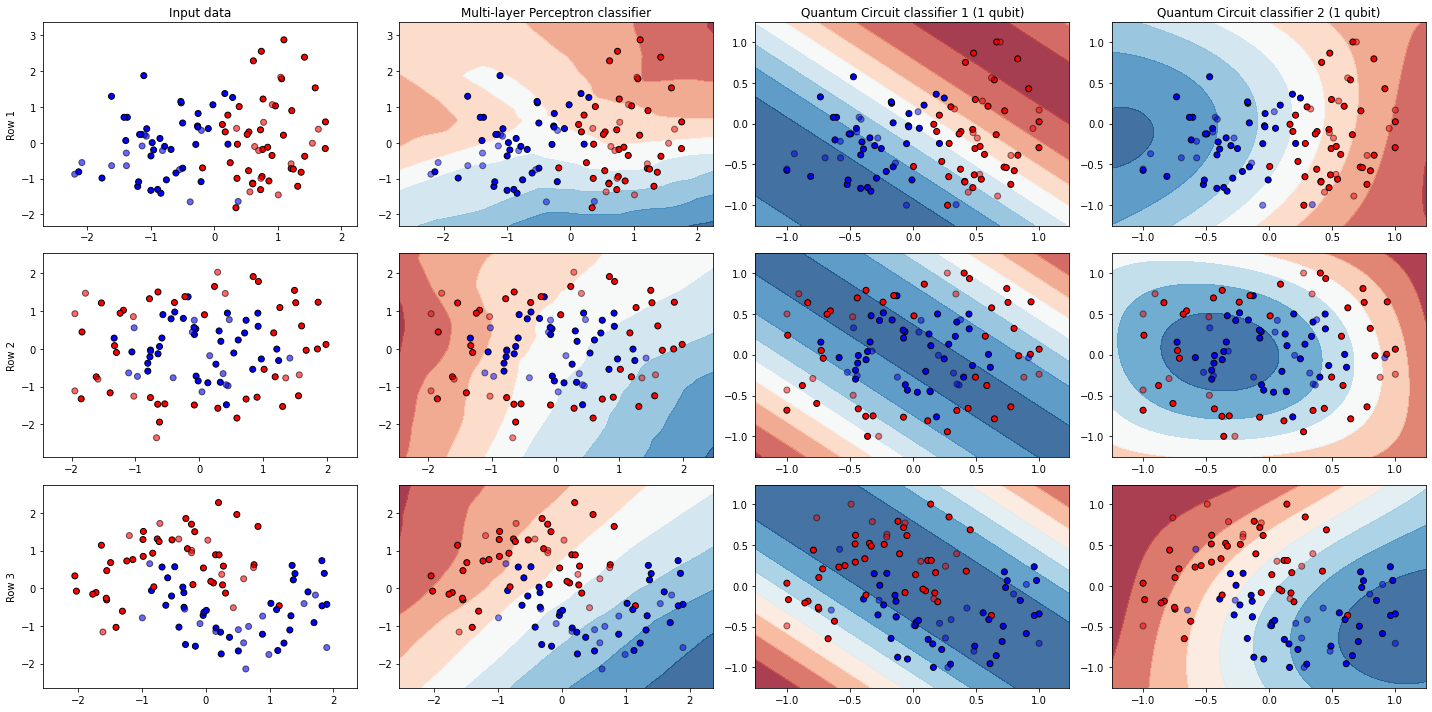
\includegraphics{Appendices/chapter_5/decision_boundary_1qubit_50-iter_01.png}
        }
        \caption{Decision boundary plot: \textbf{50 iterations} for all classifiers using \textbf{single qubit quantum circuits}.}
        \label{fig:SingleQubitClassifiers_50Iterations}
    \end{subfigure}
    \\[1ex]
    \begin{subfigure}{1.0\textwidth}
        \centering
        \begin{subfigure}{1.0\textwidth}
            \centering
            \scalebox{0.45}{
                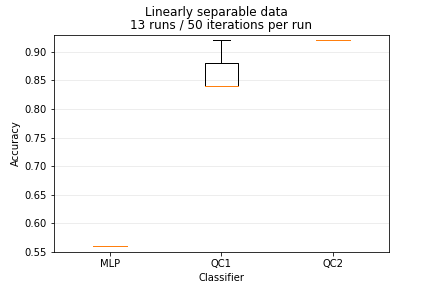
\includegraphics{Appendices/chapter_5/1qubit_Linearly_separable_data_13runs_50.png}
            }
        \end{subfigure}
        \begin{subfigure}{1.0\textwidth}
            \centering
            \scalebox{0.45}{
                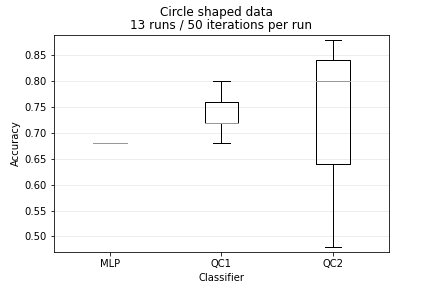
\includegraphics{Appendices/chapter_5/1qubit_Circle_shaped_data_13runs_50.png}
            }
        \end{subfigure}
        \begin{subfigure}{1.0\textwidth}
            \centering
            \scalebox{0.45}{
                 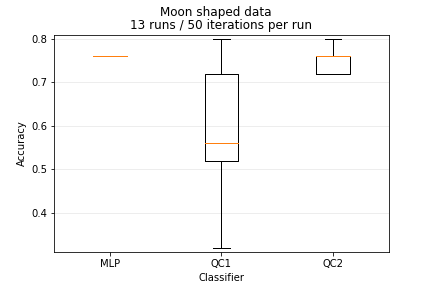
\includegraphics{Appendices/chapter_5/1qubit_Moon_shaped_data_13runs_50.png}
            }
        \end{subfigure}
        \caption{Accuracy box plots: \textbf{50 iterations} for all classifiers using \textbf{single qubit quantum circuits}.\\ \textbf{MLP}, \textbf{QC1} and \textbf{QC2} are referring to \textbf{Multi-layer Perceptron classifier}, \textbf{Quantum Circuit classifier 1} and \textbf{Quantum Circuit classifier 2} in figure \ref{fig:SingleQubitClassifiers_50Iterations} accordingly.}
        \label{fig:SingleQubitClassifiers_50Iterations_boxplot}
    \end{subfigure}
\end{figure}

\newpage
\begin{figure}[h!]
    \centering
    \caption{Decision boundary and accuracy comparison between Multi-layer Perceptron classifier, Quantum Circuit classifier 1 and Quantum Circuit classifier 2.\\\textit{Row 1}: Linearly separable data / \textit{Row 2}: Circle shaped data / \textit{Row 3}: Moon shaped data}
    \begin{subfigure}{1.0\textwidth}
        \centering
        \scalebox{0.27}{
            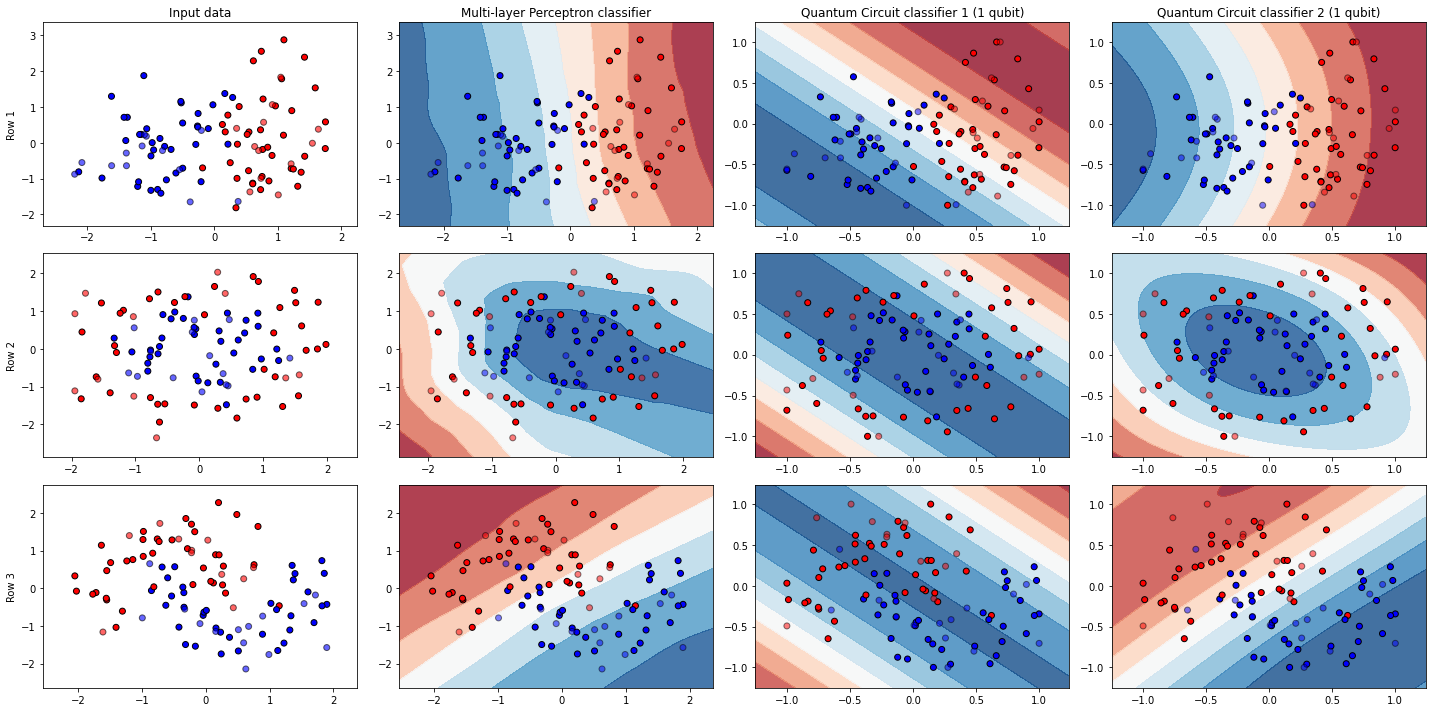
\includegraphics{Appendices/chapter_5/decision_boundary_1qubit_200-iter_01.png}
        }
        \caption{Decision boundary plot: \textbf{200 iterations} for all classifiers using \textbf{single qubit quantum circuits}.}
        \label{fig:SingleQubitClassifiers_200Iterations}
    \end{subfigure}
    \\[1ex]
    \begin{subfigure}{1.0\textwidth}
        \centering
        \begin{subfigure}{1.0\textwidth}
            \centering
            \scalebox{0.45}{
                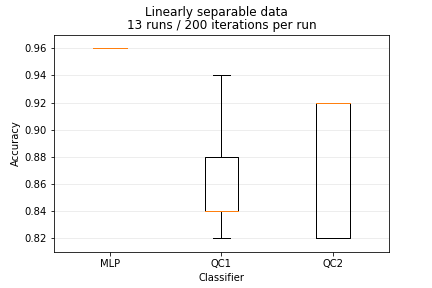
\includegraphics{Appendices/chapter_5/1qubit_Linearly_separable_data_13runs_200.png}
            }
        \end{subfigure}
        \begin{subfigure}{1.0\textwidth}
            \centering
            \scalebox{0.45}{
                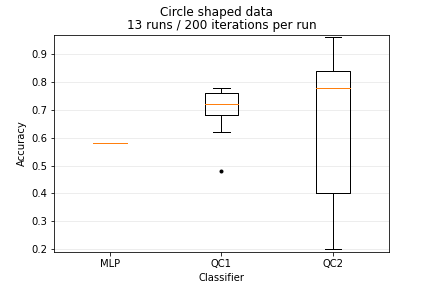
\includegraphics{Appendices/chapter_5/1qubit_Circle_shaped_data_13runs_200.png}
            }
        \end{subfigure}
        \begin{subfigure}{1.0\textwidth}
            \centering
            \scalebox{0.45}{
                 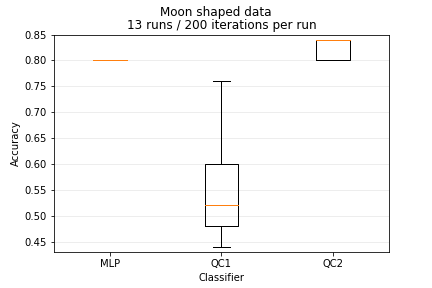
\includegraphics{Appendices/chapter_5/1qubit_Moon_shaped_data_13runs_200.png}
            }
        \end{subfigure}
        \caption{Accuracy box plots: \textbf{200 iterations} for all classifiers using \textbf{single qubit quantum circuits}.\\ \textbf{MLP}, \textbf{QC1} and \textbf{QC2} are referring to \textbf{Multi-layer Perceptron classifier}, \textbf{Quantum Circuit classifier 1} and \textbf{Quantum Circuit classifier 2} in figure \ref{fig:SingleQubitClassifiers_200Iterations} accordingly.}
        \label{fig:SingleQubitClassifiers_200Iterations_boxplot}
    \end{subfigure}
\end{figure}

\newpage
\begin{figure}[h!]
    \centering
    \caption{Decision boundary and accuracy comparison between Multi-layer Perceptron classifier, Quantum Circuit classifier 1 and Quantum Circuit classifier 2.\\\textit{Row 1}: Linearly separable data / \textit{Row 2}: Circle shaped data / \textit{Row 3}: Moon shaped data}
    \begin{subfigure}{1.0\textwidth}
        \centering
        \scalebox{0.27}{
            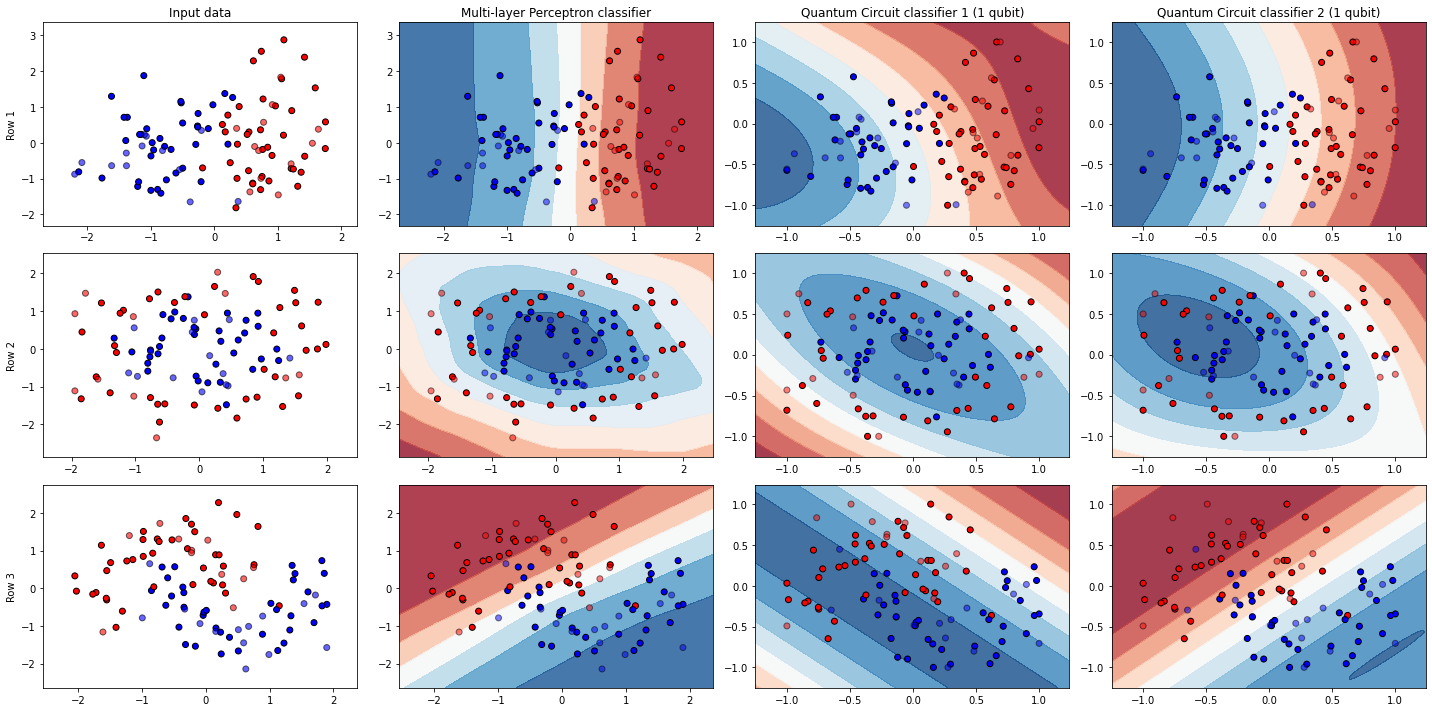
\includegraphics{Appendices/chapter_5/decision_boundary_1qubit_400-iter_01.png}
        }
        \caption{Decision boundary plot: \textbf{400 iterations} for all classifiers using \textbf{single qubit quantum circuits}.}
        \label{fig:SingleQubitClassifiers_400Iterations}
    \end{subfigure}
    \\[1ex]
    \begin{subfigure}{1.0\textwidth}
        \centering
        \begin{subfigure}{1.0\textwidth}
            \centering
            \scalebox{0.45}{
                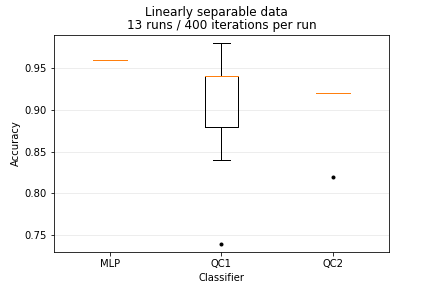
\includegraphics{Appendices/chapter_5/1qubit_Linearly_separable_data_13runs_400.png}
            }
        \end{subfigure}
        \begin{subfigure}{1.0\textwidth}
            \centering
            \scalebox{0.45}{
                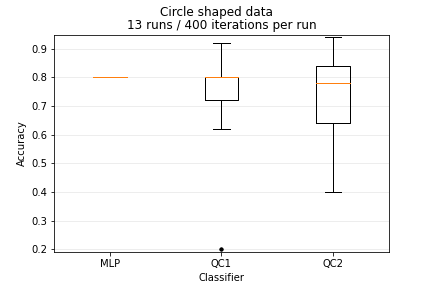
\includegraphics{Appendices/chapter_5/1qubit_Circle_shaped_data_13runs_400.png}
            }
        \end{subfigure}
        \begin{subfigure}{1.0\textwidth}
            \centering
            \scalebox{0.45}{
                 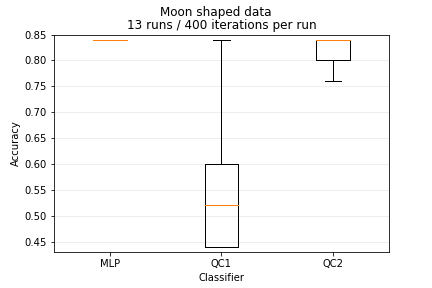
\includegraphics{Appendices/chapter_5/1qubit_Moon_shaped_data_13runs_400.png}
            }
        \end{subfigure}
        \caption{Accuracy box plots: \textbf{400 iterations} for all classifiers using \textbf{single qubit quantum circuits}.\\ \textbf{MLP}, \textbf{QC1} and \textbf{QC2} are referring to \textbf{Multi-layer Perceptron classifier}, \textbf{Quantum Circuit classifier 1} and \textbf{Quantum Circuit classifier 2} in figure \ref{fig:SingleQubitClassifiers_400Iterations} accordingly.}
        \label{fig:SingleQubitClassifiers_400Iterations_boxplot}
    \end{subfigure}
\end{figure}

\clearpage
\subsection{Two qubit circuits}
\label{subsection:two_qubit_circuits}
In this subsection, three two qubit quantum classifiers with angle embedding and a total count of six weights are trained. For comparison, there is also a Multi-layer Perceptron classifier (sklearn neural network \href{https://scikit-learn.org/stable/modules/generated/sklearn.neural_network.MLPClassifier.html}{MLPClassifier}) in the plots with the same iteration count as the quantum classifiers. Figure \ref{fig:2QubitClassifiers_50Iterations} has an iteration count of 50, figure \ref{fig:2QubitClassifiers_200Iterations} shows 200 iterations and the last figure \ref{fig:2QubitClassifiers_400Iterations} shows the classifiers after 400 iterations. The two qubit quantum classifier circuits can be seen in figures \ref{fig:two_qubit_circuit_1}, \ref{fig:two_qubit_circuit_2} and \ref{fig:two_qubit_circuit_3}.\\
\\

\begin{figure}[!h]
    \centering
    
    \begin{subfigure}{1.0\textwidth}
        \centering
        \scalebox{0.66}{
            \Qcircuit @C=1.0em @R=0.2em @!R { \\
            	 	\nghost{ {q}_{0} :  } & \lstick{ {q}_{0} :  } & \gate{\mathrm{H}} & \gate{\mathrm{R_Y}\,(\mathrm{\color{magenta}x_0})} & \ctrl{1} & \gate{\mathrm{R_Z}\,(\mathrm{\color{gray}w_0})} & \gate{\mathrm{R_Y}\,(\mathrm{\color{gray}w_1})} & \gate{\mathrm{R_Z}\,(\mathrm{\color{gray}w_2})} & \ctrl{1} & \qw & \qw\\ 
            	 	\nghost{ {q}_{1} :  } & \lstick{ {q}_{1} :  } & \gate{\mathrm{H}} & \gate{\mathrm{R_Y}\,(\mathrm{\color{magenta}x_1})} & \targ & \gate{\mathrm{R_Z}\,(\mathrm{\color{gray}w_3})} & \gate{\mathrm{R_Y}\,(\mathrm{\color{gray}w_4})} & \gate{\mathrm{R_Z}\,(\mathrm{\color{gray}w_5})} & \targ & \qw & \qw\\ 
            \\ }
        }
        \caption{\textbf{Quantum Circuit classifier 1} with starting Hadamard ($\mathrm{H}$) gates and angle embedding using a $\mathrm{RY}$ gates entangled with a $\mathrm{CX}$ gate followed by multiple $\mathrm{RY}$ and $\mathrm{RZ}$ rotation gates containing six weights in total, entangled with a final $\mathrm{CX}$ gate}
        \label{fig:two_qubit_circuit_1}
    \end{subfigure}
    \\[2ex]
    \begin{subfigure}{1.0\textwidth}
        \centering
        \scalebox{0.66}{
            \Qcircuit @C=1.0em @R=0.2em @!R { \\
            	 	\nghost{ {q}_{0} :  } & \lstick{ {q}_{0} :  } & \gate{\mathrm{H}} & \gate{\mathrm{R_Y}\,(\mathrm{\color{magenta}x_0})} & \gate{\mathrm{R_X}\,(\mathrm{\color{magenta}x_1})} & \ctrl{1} & \gate{\mathrm{R_Z}\,(\mathrm{\color{gray}w_0})} & \gate{\mathrm{R_Y}\,(\mathrm{\color{gray}w_1})} & \gate{\mathrm{R_Z}\,(\mathrm{\color{gray}w_2})} & \ctrl{1} & \qw & \qw\\ 
            	 	\nghost{ {q}_{1} :  } & \lstick{ {q}_{1} :  } & \gate{\mathrm{H}} & \qw & \qw & \targ & \gate{\mathrm{R_Z}\,(\mathrm{\color{gray}w_3})} & \gate{\mathrm{R_Y}\,(\mathrm{\color{gray}w_4})} & \gate{\mathrm{R_Z}\,(\mathrm{\color{gray}w_5})} & \targ & \qw & \qw\\ 
            \\ }
        }
        \caption{\textbf{Quantum Circuit classifier 2} differs from \textbf{Quantum Circuit classifier 1} \ref{fig:two_qubit_circuit_1} in terms of angle embedding using a $\mathrm{RY}$ and a $\mathrm{RX}$ gate to encode both features $x_0$, $x_1$ on the first qubit $q_0$ instead of using both qubits}
        \label{fig:two_qubit_circuit_2}
    \end{subfigure}
    \\[2ex]
    \begin{subfigure}{1.0\textwidth}
        \centering
        \scalebox{0.66}{
            \Qcircuit @C=1.0em @R=0.2em @!R { \\
        	 	\nghost{ {q}_{0} :  } & \lstick{ {q}_{0} :  } & \gate{\mathrm{H}} & \gate{\mathrm{R_Y}\,(\mathrm{\color{magenta}x_0})} & \ctrl{1} & \gate{\mathrm{R_Z}\,(\mathrm{\color{gray}w_0})} & \gate{\mathrm{R_Y}\,(\mathrm{\color{gray}w_1})} & \gate{\mathrm{R_Z}\,(\mathrm{\color{gray}w_2})} & \ctrl{1} & \qw & \qw\\ 
        	 	\nghost{ {q}_{1} :  } & \lstick{ {q}_{1} :  } & \gate{\mathrm{H}} & \gate{\mathrm{R_X}\,(\mathrm{\color{magenta}x_1})} & \targ & \gate{\mathrm{R_Z}\,(\mathrm{\color{gray}w_3})} & \gate{\mathrm{R_Y}\,(\mathrm{\color{gray}w_4})} & \gate{\mathrm{R_Z}\,(\mathrm{\color{gray}w_5})} & \targ & \qw & \qw\\ 
            \\ }
        }
        \caption{\textbf{Quantum Circuit classifier 3} with starting Hadamard ($\mathrm{H}$) gates and angle embedding using a $\mathrm{RY}$ and a $\mathrm{RX}$ gate}
        \label{fig:two_qubit_circuit_3}
    \end{subfigure}
    
    \caption{Two qubit quantum circuits referring to the \textbf{Quantum Circuit classifier 1}, \textbf{Quantum Circuit classifier 2} and \textbf{Quantum Circuit classifier 3} in figures \ref{fig:2QubitClassifiers_50Iterations}, \ref{fig:2QubitClassifiers_200Iterations} and \ref{fig:2QubitClassifiers_400Iterations}.}
    \label{fig:two_qubit_circuits}
\end{figure}

% Contour and box plots
\begin{figure}[!h]
    \centering
    \caption{Decision boundary and accuracy comparison between Multi-layer Perceptron classifier, Quantum Circuit classifier 1, Quantum Circuit classifier 2 and Quantum Circuit classifier 3.\\\textit{Row 1}: Linearly separable data / \textit{Row 2}: Circle shaped data / \textit{Row 3}: Moon shaped data}
    \begin{subfigure}{1.0\textwidth}
        \centering
        \scalebox{0.27}{
            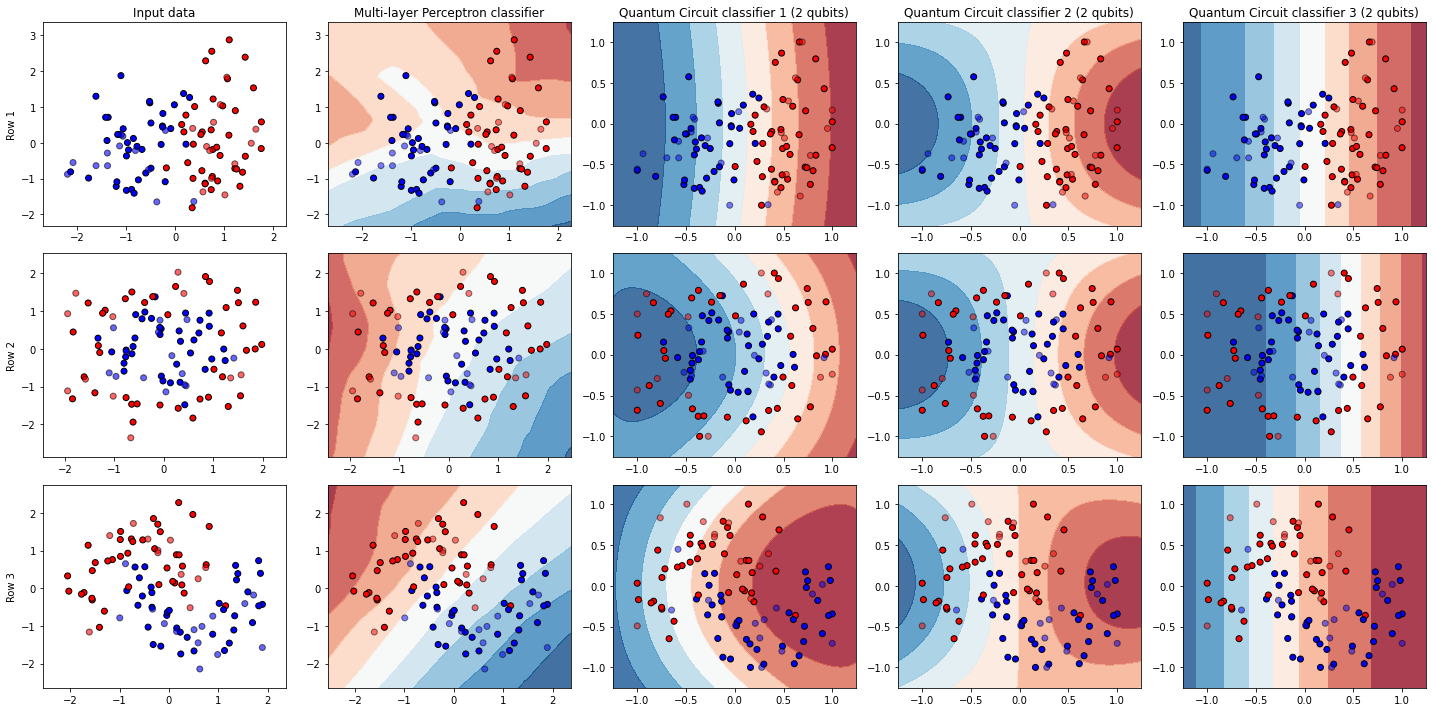
\includegraphics{Appendices/chapter_5/decision_boundary_2qubits_50-iter_01.png}
        }
        \caption{\textbf{50 iterations} for all classifiers using \textbf{two qubit quantum circuits}.}
        \label{fig:2QubitClassifiers_50Iterations}
    \end{subfigure}
    \\[1ex]
    \begin{subfigure}{1.0\textwidth}
        \centering
        \begin{subfigure}{1.0\textwidth}
            \centering
            \scalebox{0.45}{
                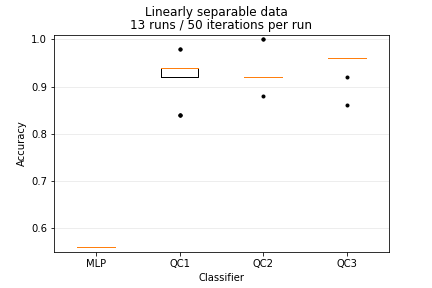
\includegraphics{Appendices/chapter_5/2qubits_Linearly_separable_data_13runs_50.png}
            }
        \end{subfigure}
        \begin{subfigure}{1.0\textwidth}
            \centering
            \scalebox{0.45}{
                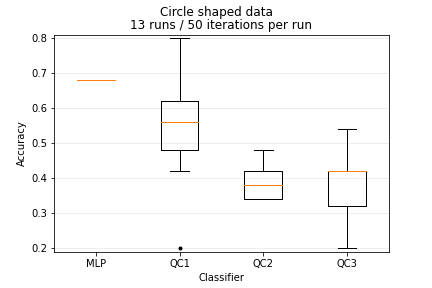
\includegraphics{Appendices/chapter_5/2qubits_Circle_shaped_data_13runs_50.png}
            }
        \end{subfigure}
        \begin{subfigure}{1.0\textwidth}
            \centering
            \scalebox{0.45}{
                 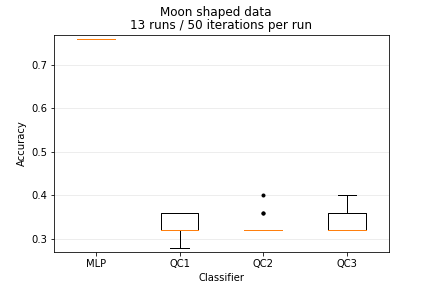
\includegraphics{Appendices/chapter_5/2qubits_Moon_shaped_data_13runs_50.png}
            }
        \end{subfigure}
        \caption{Accuracy box plots: \textbf{50 iterations} for all classifiers using \textbf{two qubit quantum circuits}.\\ \textbf{MLP}, \textbf{QC1}, \textbf{QC2} and \textbf{QC3} are referring to \textbf{Multi-layer Perceptron classifier}, \textbf{Quantum Circuit classifier 1}, \textbf{Quantum Circuit classifier 2} and \textbf{Quantum Circuit classifier 3} in figure \ref{fig:2QubitClassifiers_50Iterations} accordingly.}
        \label{fig:2QubitClassifiers_50Iterations_boxplot}
    \end{subfigure}
\end{figure}

\newpage
\begin{figure}[!h]
    \centering
    \caption{Decision boundary and accuracy comparison between Multi-layer Perceptron classifier, Quantum Circuit classifier 1, Quantum Circuit classifier 2 and Quantum Circuit classifier 3.\\\textit{Row 1}: Linearly separable data / \textit{Row 2}: Circle shaped data / \textit{Row 3}: Moon shaped data}
    \begin{subfigure}{1.0\textwidth}
        \centering
        \scalebox{0.27}{
            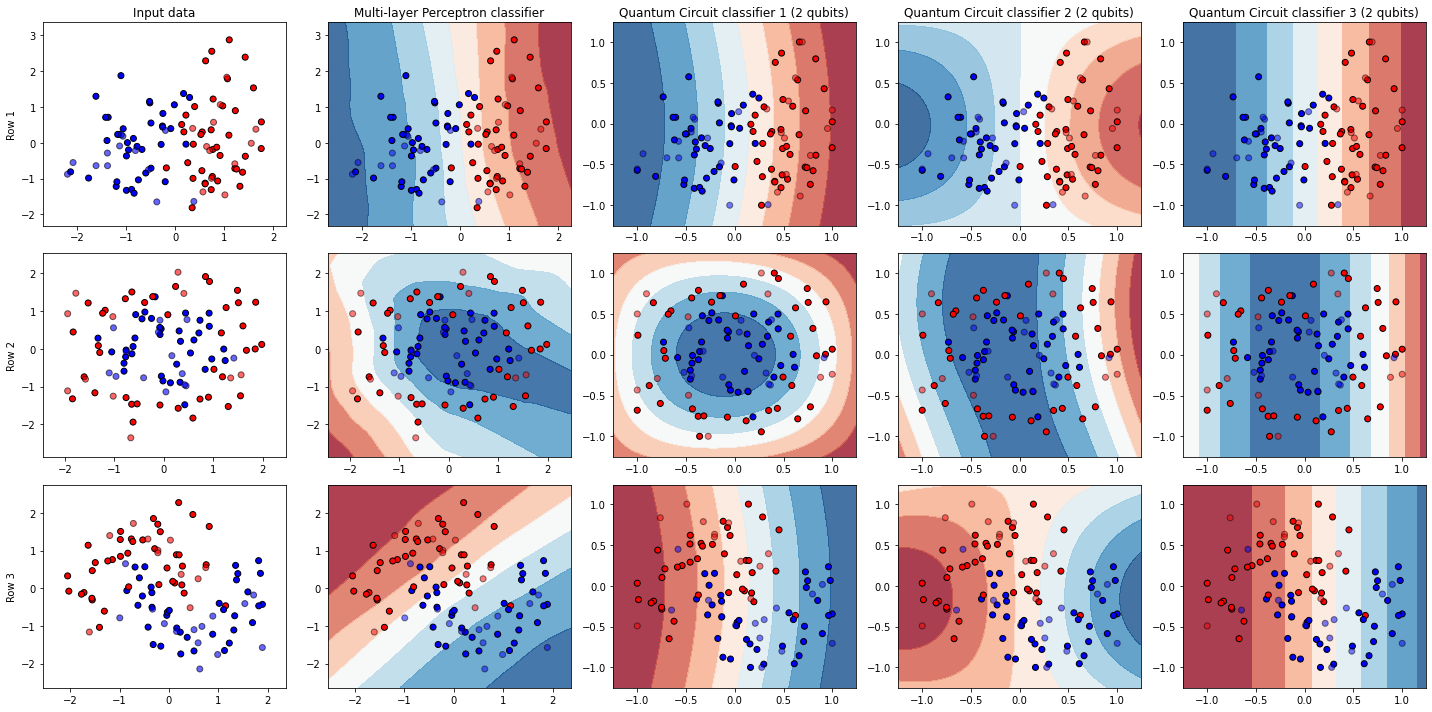
\includegraphics{Appendices/chapter_5/decision_boundary_2qubits_200-iter_01.png}
        }
        \caption{\textbf{200 iterations} for all classifiers using \textbf{two qubit quantum circuits}.}
        \label{fig:2QubitClassifiers_200Iterations}
    \end{subfigure}
    \\[1ex]
    \begin{subfigure}{1.0\textwidth}
        \centering
        \begin{subfigure}{1.0\textwidth}
            \centering
            \scalebox{0.45}{
                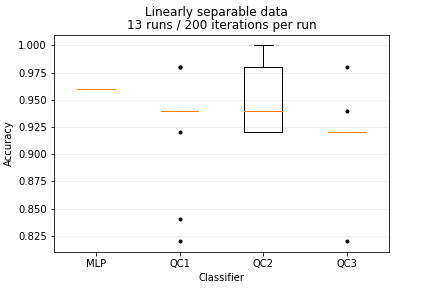
\includegraphics{Appendices/chapter_5/2qubits_Linearly_separable_data_13runs_200.png}
            }
        \end{subfigure}
        \begin{subfigure}{1.0\textwidth}
            \centering
            \scalebox{0.45}{
                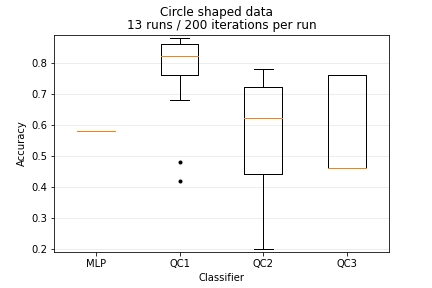
\includegraphics{Appendices/chapter_5/2qubits_Circle_shaped_data_13runs_200.png}
            }
        \end{subfigure}
        \begin{subfigure}{1.0\textwidth}
            \centering
            \scalebox{0.45}{
                 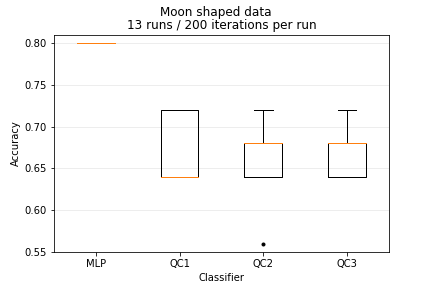
\includegraphics{Appendices/chapter_5/2qubits_Moon_shaped_data_13runs_200.png}
            }
        \end{subfigure}
        \caption{Accuracy box plots: \textbf{200 iterations} for all classifiers using \textbf{two qubit quantum circuits}.\\ \textbf{MLP}, \textbf{QC1}, \textbf{QC2} and \textbf{QC3} are referring to \textbf{Multi-layer Perceptron classifier}, \textbf{Quantum Circuit classifier 1}, \textbf{Quantum Circuit classifier 2} and \textbf{Quantum Circuit classifier 3} in figure \ref{fig:2QubitClassifiers_200Iterations} accordingly.}
        \label{fig:2QubitClassifiers_200Iterations_boxplot}
    \end{subfigure}
\end{figure}

\newpage
\begin{figure}[!h]
    \centering
    \caption{Decision boundary and accuracy comparison between Multi-layer Perceptron classifier, Quantum Circuit classifier 1, Quantum Circuit classifier 2 and Quantum Circuit classifier 3.\\\textit{Row 1}: Linearly separable data / \textit{Row 2}: Circle shaped data / \textit{Row 3}: Moon shaped data}
    \begin{subfigure}{1.0\textwidth}
        \centering
        \scalebox{0.27}{
            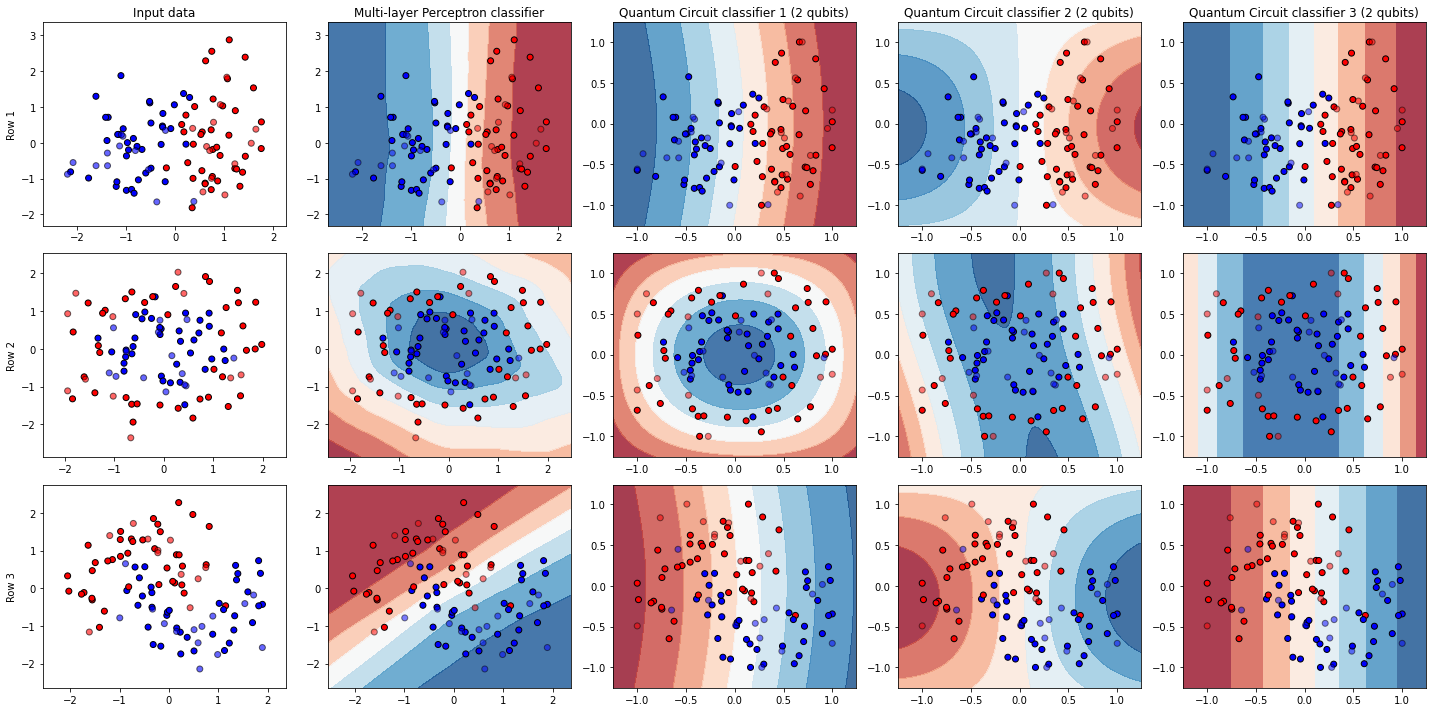
\includegraphics{Appendices/chapter_5/decision_boundary_2qubits_400-iter_01.png}
        }
        \caption{\textbf{400 iterations} for all classifiers using \textbf{two qubit quantum circuits}.}
        \label{fig:2QubitClassifiers_400Iterations}
    \end{subfigure}
    \\[1ex]
    \begin{subfigure}{1.0\textwidth}
        \centering
        \begin{subfigure}{1.0\textwidth}
            \centering
            \scalebox{0.45}{
                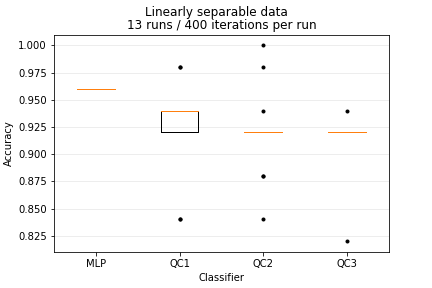
\includegraphics{Appendices/chapter_5/2qubits_Linearly_separable_data_13runs_400.png}
            }
        \end{subfigure}
        \begin{subfigure}{1.0\textwidth}
            \centering
            \scalebox{0.45}{
                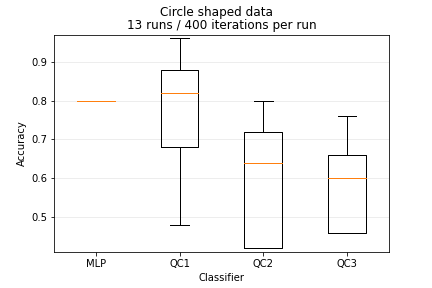
\includegraphics{Appendices/chapter_5/2qubits_Circle_shaped_data_13runs_400.png}
            }
        \end{subfigure}
        \begin{subfigure}{1.0\textwidth}
            \centering
            \scalebox{0.45}{
                 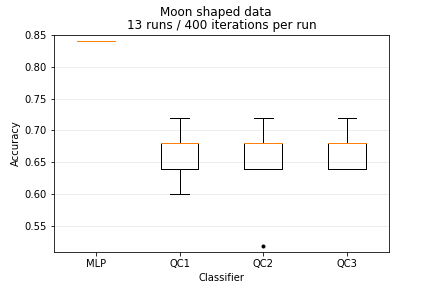
\includegraphics{Appendices/chapter_5/2qubits_Moon_shaped_data_13runs_400.png}
            }
        \end{subfigure}
        \caption{Accuracy box plots: \textbf{400 iterations} for all classifiers using \textbf{two qubit quantum circuits}.\\ \textbf{MLP}, \textbf{QC1}, \textbf{QC2} and \textbf{QC3} are referring to \textbf{Multi-layer Perceptron classifier}, \textbf{Quantum Circuit classifier 1}, \textbf{Quantum Circuit classifier 2} and \textbf{Quantum Circuit classifier 3} in figure \ref{fig:2QubitClassifiers_400Iterations} accordingly.}
        \label{fig:2QubitClassifiers_400Iterations_boxplot}
    \end{subfigure}
\end{figure}

\clearpage
\subsection{Two qubit circuits with 3 layers}
\label{subsection:two_qubit_circuits_3layers}

In this subsection, three two qubit quantum classifiers with three layers (the same quantum circuits as in subsection \ref{subsection:two_qubit_circuits} repeated three times, excluding the Hadamard ($\mathrm{H}$) gates) using angle embedding and a total count of $3\times6 = 18$ weights have been trained. Again for comparison, there is also a Multi-layer Perceptron classifier (sklearn neural network \href{https://scikit-learn.org/stable/modules/generated/sklearn.neural_network.MLPClassifier.html}{MLPClassifier}) in the plots with the same iteration count as the quantum classifiers, but this time with 3 hidden layers as seen in figure \ref{fig:code_MLPClassifier_configuration_3hiddenlayers}. Figure \ref{fig:2Qubit3LayersClassifiers_50Iterations} has an iteration count of 50, figure \ref{fig:2Qubit3LayersClassifiers_200Iterations} shows 200 iterations and the last figure \ref{fig:2Qubit3LayersClassifiers_400Iterations} shows the classifiers after 400 iterations. The two qubit quantum classifiers with three layer circuits can be seen in figures \ref{fig:two_qubit_3layers_circuit_1}, \ref{fig:two_qubit_3layers_circuit_2} and \ref{fig:two_qubit_3layers_circuit_3}.\\

\hfill \break

\begin{figure}[!h]
    \centering
    
    \begin{subfigure}{1.0\textwidth}
        \centering
        \scalebox{0.43}{
            \Qcircuit @C=1.0em @R=0.2em @!R { \\
            	 	\nghost{ {q}_{0} :  } & \lstick{ {q}_{0} :  } & \gate{\mathrm{H}} \barrier[0em]{1} & \qw & \gate{\mathrm{R_Y}\,(\mathrm{\color{magenta}x_0})} & \ctrl{1} & \gate{\mathrm{R_Z}\,(\mathrm{\color{gray}w_0})} & \gate{\mathrm{R_Y}\,(\mathrm{\color{gray}w_1})} & \gate{\mathrm{R_Z}\,(\mathrm{\color{gray}w_2})} & \ctrl{1} \barrier[0em]{1} & \qw & \gate{\mathrm{R_Y}\,(\mathrm{\color{magenta}x_0})} & \ctrl{1} & \gate{\mathrm{R_Z}\,(\mathrm{\color{gray}w_6})} & \gate{\mathrm{R_Y}\,(\mathrm{\color{gray}w_7})} & \gate{\mathrm{R_Z}\,(\mathrm{\color{gray}w_8})} & \ctrl{1} \barrier[0em]{1} & \qw & \gate{\mathrm{R_Y}\,(\mathrm{\color{magenta}x_0})} & \ctrl{1} & \gate{\mathrm{R_Z}\,(\mathrm{\color{gray}w_{12}})} & \gate{\mathrm{R_Y}\,(\mathrm{\color{gray}w_{13}})} & \gate{\mathrm{R_Z}\,(\mathrm{\color{gray}w_{14}})} & \ctrl{1} & \qw & \qw\\ 
            	 	\nghost{ {q}_{1} :  } & \lstick{ {q}_{1} :  } & \gate{\mathrm{H}} & \qw & \gate{\mathrm{R_Y}\,(\mathrm{\color{magenta}x_1})} & \targ & \gate{\mathrm{R_Z}\,(\mathrm{\color{gray}w_3})} & \gate{\mathrm{R_Y}\,(\mathrm{\color{gray}w_4})} & \gate{\mathrm{R_Z}\,(\mathrm{\color{gray}w_5})} & \targ & \qw & \gate{\mathrm{R_Y}\,(\mathrm{\color{magenta}x_1})} & \targ & \gate{\mathrm{R_Z}\,(\mathrm{\color{gray}w_9})} & \gate{\mathrm{R_Y}\,(\mathrm{\color{gray}w_{10}})} & \gate{\mathrm{R_Z}\,(\mathrm{\color{gray}w_{11}})} & \targ & \qw & \gate{\mathrm{R_Y}\,(\mathrm{\color{magenta}x_1})} & \targ & \gate{\mathrm{R_Z}\,(\mathrm{\color{gray}w_{15}})} & \gate{\mathrm{R_Y}\,(\mathrm{\color{gray}w_{16}})} & \gate{\mathrm{R_Z}\,(\mathrm{\color{gray}w_{17}})} & \targ & \qw & \qw\\ 
            \\ }
        }
        \caption{\textbf{Quantum Circuit classifier 1} same as the two qubit classifier in figure \ref{fig:two_qubit_circuit_1} with 2 additional "layers"}
        \label{fig:two_qubit_3layers_circuit_1}
    \end{subfigure}
    \\[2ex]
    \begin{subfigure}{1.0\textwidth}
        \centering
        \scalebox{0.37}{
            \Qcircuit @C=1.0em @R=0.2em @!R { \\
            	 	\nghost{ {q}_{0} :  } & \lstick{ {q}_{0} :  } & \gate{\mathrm{H}} \barrier[0em]{1} & \qw & \gate{\mathrm{R_Y}\,(\mathrm{\color{magenta}x_0})} & \gate{\mathrm{R_X}\,(\mathrm{\color{magenta}x_1})} & \ctrl{1} & \gate{\mathrm{R_Z}\,(\mathrm{\color{gray}w_0})} & \gate{\mathrm{R_Y}\,(\mathrm{\color{gray}w_1})} & \gate{\mathrm{R_Z}\,(\mathrm{\color{gray}w_2})} & \ctrl{1} \barrier[0em]{1} & \qw & \gate{\mathrm{R_Y}\,(\mathrm{\color{magenta}x_0})} & \gate{\mathrm{R_X}\,(\mathrm{\color{magenta}x_1})} & \ctrl{1} & \gate{\mathrm{R_Z}\,(\mathrm{\color{gray}w_6})} & \gate{\mathrm{R_Y}\,(\mathrm{\color{gray}w_7})} & \gate{\mathrm{R_Z}\,(\mathrm{\color{gray}w_8})} & \ctrl{1} \barrier[0em]{1} & \qw & \gate{\mathrm{R_Y}\,(\mathrm{\color{magenta}x_0})} & \gate{\mathrm{R_X}\,(\mathrm{\color{magenta}x_1})} & \ctrl{1} & \gate{\mathrm{R_Z}\,(\mathrm{\color{gray}w_{12}})} & \gate{\mathrm{R_Y}\,(\mathrm{\color{gray}w_{13}})} & \gate{\mathrm{R_Z}\,(\mathrm{\color{gray}w_{14}})} & \ctrl{1} & \qw & \qw\\ 
            	 	\nghost{ {q}_{1} :  } & \lstick{ {q}_{1} :  } & \gate{\mathrm{H}} & \qw & \qw & \qw & \targ & \gate{\mathrm{R_Z}\,(\mathrm{\color{gray}w_3})} & \gate{\mathrm{R_Y}\,(\mathrm{\color{gray}w_4})} & \gate{\mathrm{R_Z}\,(\mathrm{\color{gray}w_5})} & \targ & \qw & \qw & \qw & \targ & \gate{\mathrm{R_Z}\,(\mathrm{\color{gray}w_9})} & \gate{\mathrm{R_Y}\,(\mathrm{\color{gray}w_{10}})} & \gate{\mathrm{R_Z}\,(\mathrm{\color{gray}w_{11}})} & \targ & \qw & \qw & \qw & \targ & \gate{\mathrm{R_Z}\,(\mathrm{\color{gray}w_{15}})} & \gate{\mathrm{R_Y}\,(\mathrm{\color{gray}w_{16}})} & \gate{\mathrm{R_Z}\,(\mathrm{\color{gray}w_{17}})} & \targ & \qw & \qw\\ 
            \\ }
        }
        \caption{\textbf{Quantum Circuit classifier 2} same as the two qubit classifier in figure \ref{fig:two_qubit_circuit_2} with 2 additional "layers"}
        \label{fig:two_qubit_3layers_circuit_2}
    \end{subfigure}
    \\[2ex]
    \begin{subfigure}{1.0\textwidth}
        \centering
        \scalebox{0.43}{
            \Qcircuit @C=1.0em @R=0.2em @!R { \\
            	 	\nghost{ {q}_{0} :  } & \lstick{ {q}_{0} :  } & \gate{\mathrm{H}} \barrier[0em]{1} & \qw & \gate{\mathrm{R_Y}\,(\mathrm{\color{magenta}x_0})} & \ctrl{1} & \gate{\mathrm{R_Z}\,(\mathrm{\color{gray}w_0})} & \gate{\mathrm{R_Y}\,(\mathrm{\color{gray}w_1})} & \gate{\mathrm{R_Z}\,(\mathrm{\color{gray}w_2})} & \ctrl{1} \barrier[0em]{1} & \qw & \gate{\mathrm{R_Y}\,(\mathrm{\color{magenta}x_0})} & \ctrl{1} & \gate{\mathrm{R_Z}\,(\mathrm{\color{gray}w_6})} & \gate{\mathrm{R_Y}\,(\mathrm{\color{gray}w_7})} & \gate{\mathrm{R_Z}\,(\mathrm{\color{gray}w_8})} & \ctrl{1} \barrier[0em]{1} & \qw & \gate{\mathrm{R_Y}\,(\mathrm{\color{magenta}x_0})} & \ctrl{1} & \gate{\mathrm{R_Z}\,(\mathrm{\color{gray}w_{12}})} & \gate{\mathrm{R_Y}\,(\mathrm{\color{gray}w_{13}})} & \gate{\mathrm{R_Z}\,(\mathrm{\color{gray}w_{14}})} & \ctrl{1} & \qw & \qw\\ 
            	 	\nghost{ {q}_{1} :  } & \lstick{ {q}_{1} :  } & \gate{\mathrm{H}} & \qw & \gate{\mathrm{R_X}\,(\mathrm{\color{magenta}x_1})} & \targ & \gate{\mathrm{R_Z}\,(\mathrm{\color{gray}w_3})} & \gate{\mathrm{R_Y}\,(\mathrm{\color{gray}w_4})} & \gate{\mathrm{R_Z}\,(\mathrm{\color{gray}w_5})} & \targ & \qw & \gate{\mathrm{R_X}\,(\mathrm{\color{magenta}x_1})} & \targ & \gate{\mathrm{R_Z}\,(\mathrm{\color{gray}w_9})} & \gate{\mathrm{R_Y}\,(\mathrm{\color{gray}w_{10}})} & \gate{\mathrm{R_Z}\,(\mathrm{\color{gray}w_{11}})} & \targ & \qw & \gate{\mathrm{R_X}\,(\mathrm{\color{magenta}x_1})} & \targ & \gate{\mathrm{R_Z}\,(\mathrm{\color{gray}w_{15}})} & \gate{\mathrm{R_Y}\,(\mathrm{\color{gray}w_{16}})} & \gate{\mathrm{R_Z}\,(\mathrm{\color{gray}w_{17}})} & \targ & \qw & \qw\\ 
            \\ }
        }
        \caption{\textbf{Quantum Circuit classifier 3} same as the two qubit classifier in figure \ref{fig:two_qubit_circuit_3} with 2 additional "layers"}
        \label{fig:two_qubit_3layers_circuit_3}
    \end{subfigure}
    
    \caption{Two qubit quantum circuits with 3 layers referring to the \textbf{Quantum Circuit classifier 1}, \textbf{Quantum Circuit classifier 2} and \textbf{Quantum Circuit classifier 3} in figures \ref{fig:2Qubit3LayersClassifiers_50Iterations}, \ref{fig:2Qubit3LayersClassifiers_200Iterations} and \ref{fig:2Qubit3LayersClassifiers_400Iterations}. For better visual understanding three barriers have been added, marking the beginning of each layer. The barriers have no impact on the circuits themselves and are only used for visualization purposes.}
    \label{fig:two_qubit_3layers_circuits}
\end{figure}

% Contour and box plots
\begin{figure}[!h]
    \centering
    \caption{Decision boundary and accuracy comparison between Multi-layer Perceptron classifier, Quantum Circuit classifier 1, Quantum Circuit classifier 2 and Quantum Circuit classifier 3.\\\textit{Row 1}: Linearly separable data / \textit{Row 2}: Circle shaped data / \textit{Row 3}: Moon shaped data}
    \begin{subfigure}{1.0\textwidth}
        \centering
        \scalebox{0.27}{
            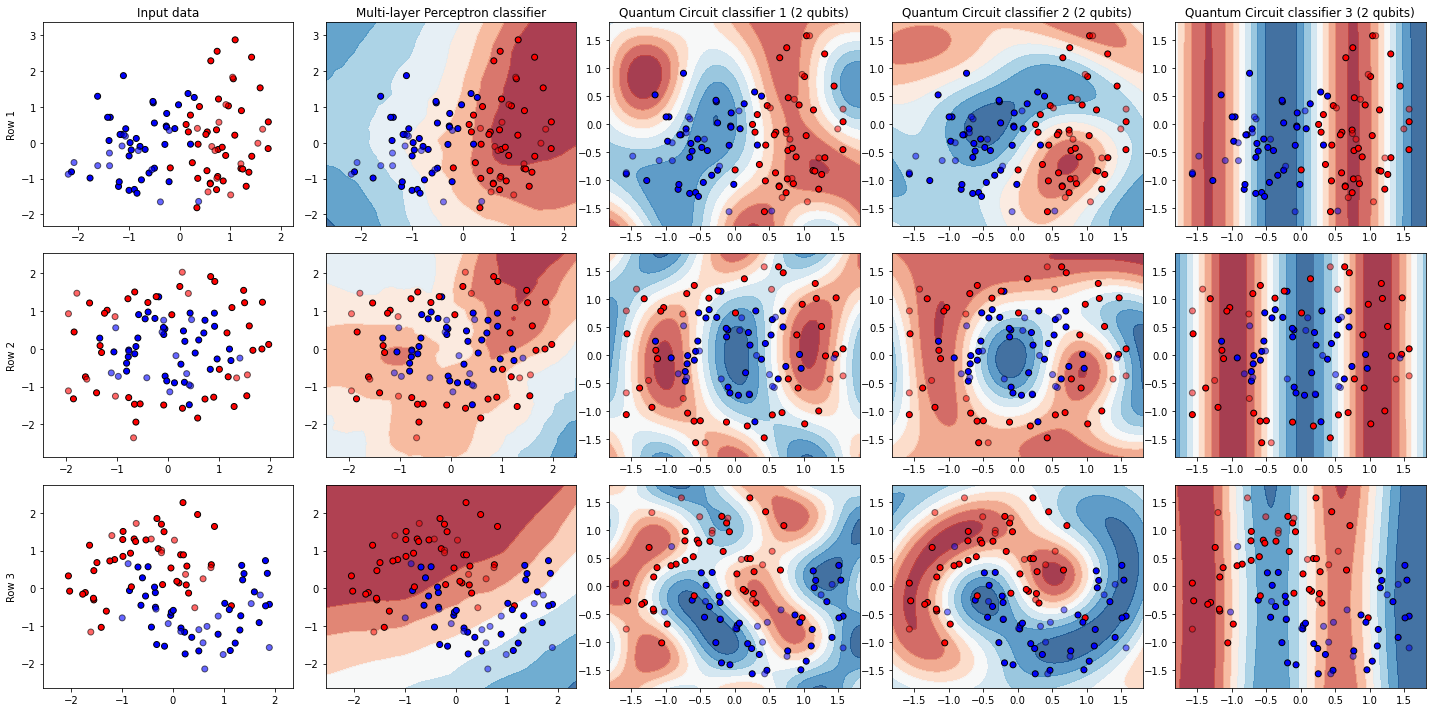
\includegraphics{Appendices/chapter_5/decision_boundary_2qubits_3layers_50-iter_01.png}
        }
        \caption{\textbf{50 iterations} for all classifiers using \textbf{two qubit quantum circuits with 3 layers}.}
        \label{fig:2Qubit3LayersClassifiers_50Iterations}
    \end{subfigure}
    \\[1ex]
    \begin{subfigure}{1.0\textwidth}
        \centering
        \begin{subfigure}{1.0\textwidth}
            \centering
            \scalebox{0.45}{
                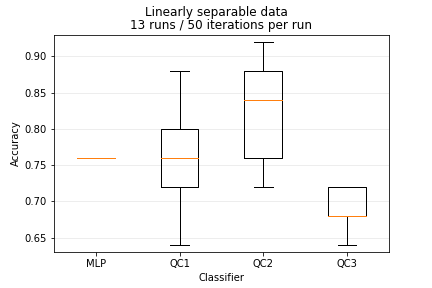
\includegraphics{Appendices/chapter_5/2qubits_3layers_Linearly_separable_data_13runs_50.png}
            }
        \end{subfigure}
        \begin{subfigure}{1.0\textwidth}
            \centering
            \scalebox{0.45}{
                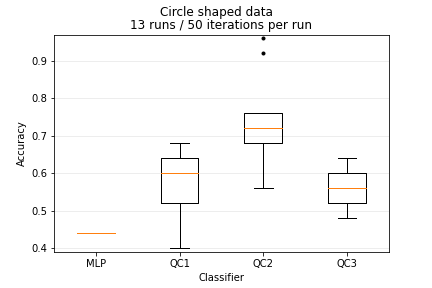
\includegraphics{Appendices/chapter_5/2qubits_3layers_Circle_shaped_data_13runs_50.png}
            }
        \end{subfigure}
        \begin{subfigure}{1.0\textwidth}
            \centering
            \scalebox{0.45}{
                 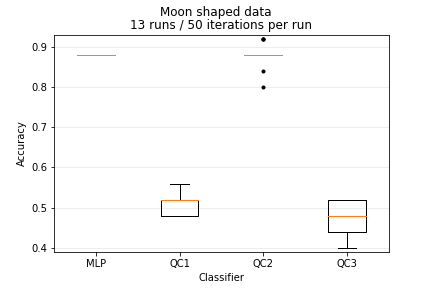
\includegraphics{Appendices/chapter_5/2qubits_3layers_Moon_shaped_data_13runs_50.png}
            }
        \end{subfigure}
        \caption{Accuracy box plots: \textbf{50 iterations} for all classifiers using \textbf{two qubit quantum circuits with 3 layers}.\\ \textbf{MLP}, \textbf{QC1}, \textbf{QC2} and \textbf{QC3} are referring to \textbf{Multi-layer Perceptron classifier}, \textbf{Quantum Circuit classifier 1}, \textbf{Quantum Circuit classifier 2} and \textbf{Quantum Circuit classifier 3} in figure \ref{fig:2Qubit3LayersClassifiers_50Iterations} accordingly.}
        \label{fig:2Qubit3LayersClassifiers_50Iterations_boxplot}
    \end{subfigure}
\end{figure}

\newpage
\begin{figure}[!h]
    \centering
    \caption{Decision boundary and accuracy comparison between Multi-layer Perceptron classifier, Quantum Circuit classifier 1, Quantum Circuit classifier 2 and Quantum Circuit classifier 3.\\\textit{Row 1}: Linearly separable data / \textit{Row 2}: Circle shaped data / \textit{Row 3}: Moon shaped data}
    \begin{subfigure}{1.0\textwidth}
        \centering
        \scalebox{0.27}{
            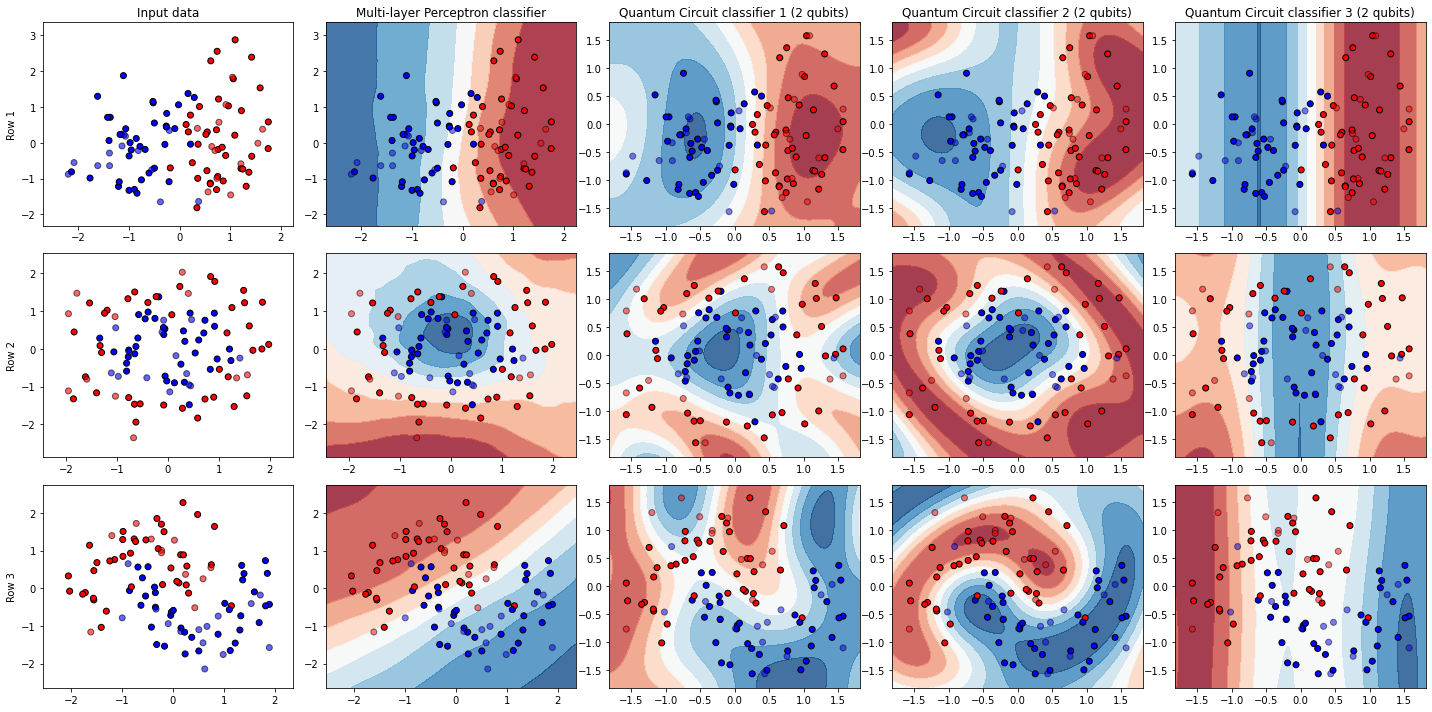
\includegraphics{Appendices/chapter_5/decision_boundary_2qubits_3layers_200-iter_01.png}
        }
        \caption{\textbf{200 iterations} for all classifiers using \textbf{two qubit quantum circuits with 3 layers}.}
        \label{fig:2Qubit3LayersClassifiers_200Iterations}
    \end{subfigure}
    \\[1ex]
    \begin{subfigure}{1.0\textwidth}
        \centering
        \begin{subfigure}{1.0\textwidth}
            \centering
            \scalebox{0.45}{
                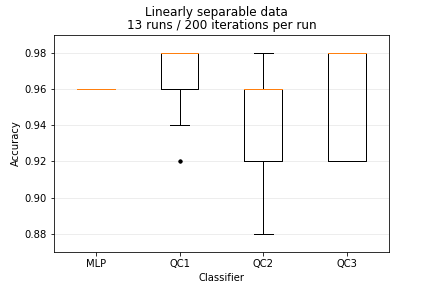
\includegraphics{Appendices/chapter_5/2qubits_3layers_Linearly_separable_data_13runs_200.png}
            }
        \end{subfigure}
        \begin{subfigure}{1.0\textwidth}
            \centering
            \scalebox{0.45}{
                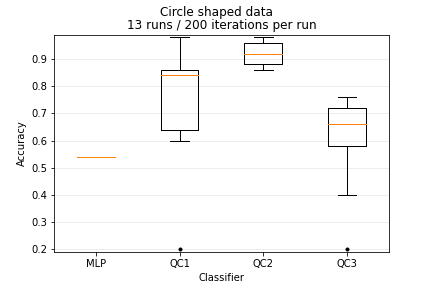
\includegraphics{Appendices/chapter_5/2qubits_3layers_Circle_shaped_data_13runs_200.png}
            }
        \end{subfigure}
        \begin{subfigure}{1.0\textwidth}
            \centering
            \scalebox{0.45}{
                 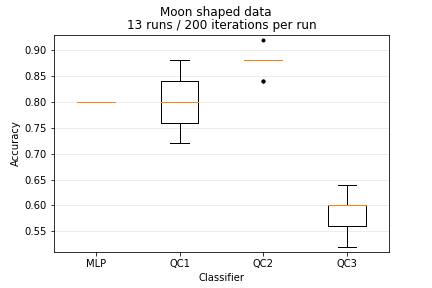
\includegraphics{Appendices/chapter_5/2qubits_3layers_Moon_shaped_data_13runs_200.png}
            }
        \end{subfigure}
        \caption{Accuracy box plots: \textbf{200 iterations} for all classifiers using \textbf{two qubit quantum circuits with 3 layers}.\\ \textbf{MLP}, \textbf{QC1}, \textbf{QC2} and \textbf{QC3} are referring to \textbf{Multi-layer Perceptron classifier}, \textbf{Quantum Circuit classifier 1}, \textbf{Quantum Circuit classifier 2} and \textbf{Quantum Circuit classifier 3} in figure \ref{fig:2Qubit3LayersClassifiers_200Iterations} accordingly.}
        \label{fig:2Qubit3LayersClassifiers_200Iterations_boxplot}
    \end{subfigure}
\end{figure}

\newpage
\begin{figure}[!h]
    \centering
    \caption{Decision boundary and accuracy comparison between Multi-layer Perceptron classifier, Quantum Circuit classifier 1, Quantum Circuit classifier 2 and Quantum Circuit classifier 3.\\\textit{Row 1}: Linearly separable data / \textit{Row 2}: Circle shaped data / \textit{Row 3}: Moon shaped data}
    \begin{subfigure}{1.0\textwidth}
        \centering
        \scalebox{0.27}{
            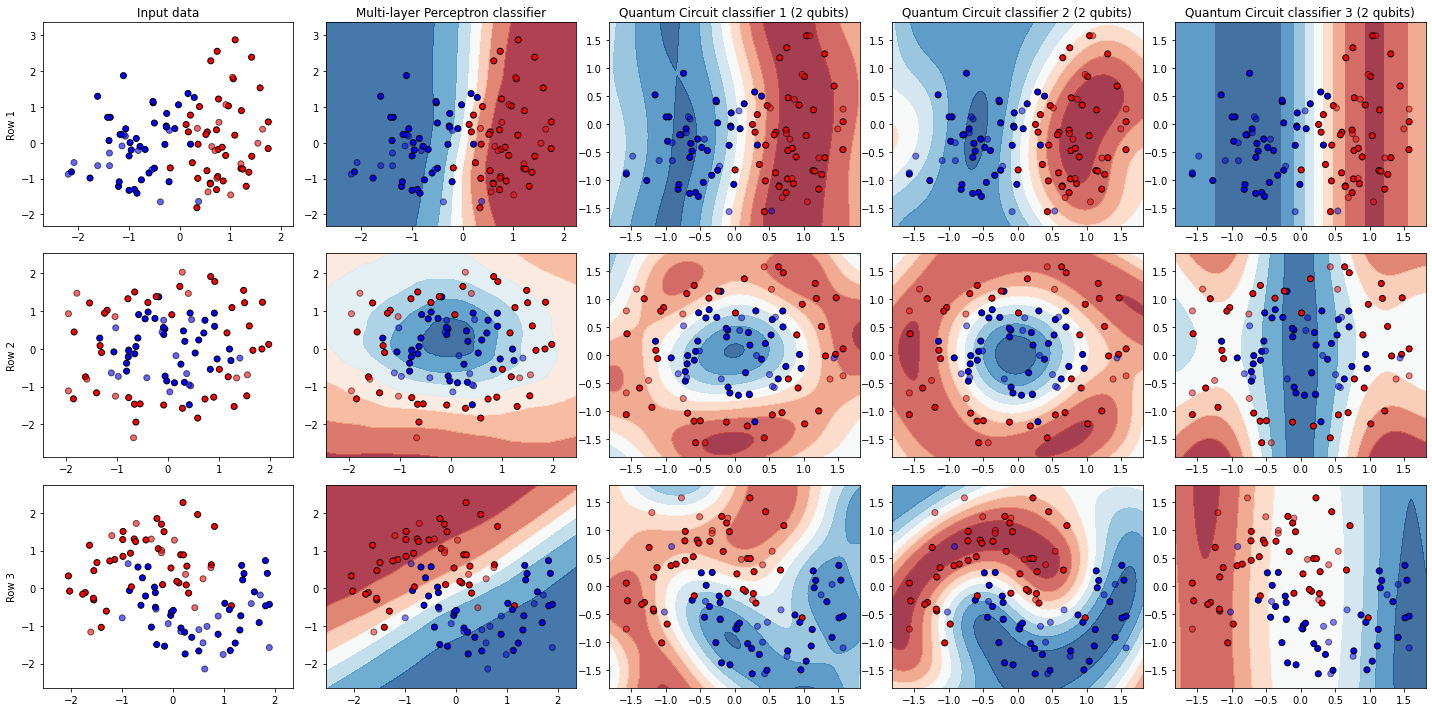
\includegraphics{Appendices/chapter_5/decision_boundary_2qubits_3layers_400-iter_01.png}
        }
        \caption{\textbf{400 iterations} for all classifiers using \textbf{two qubit quantum circuits with 3 layers}.}
        \label{fig:2Qubit3LayersClassifiers_400Iterations}
    \end{subfigure}
    \\[1ex]
    \begin{subfigure}{1.0\textwidth}
        \centering
        \begin{subfigure}{1.0\textwidth}
            \centering
            \scalebox{0.45}{
                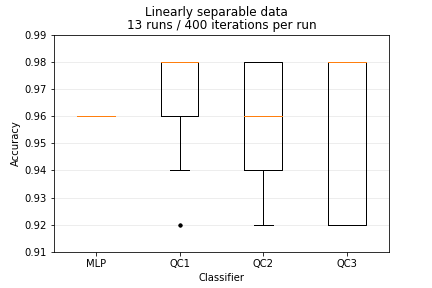
\includegraphics{Appendices/chapter_5/2qubits_3layers_Linearly_separable_data_13runs_400.png}
            }
        \end{subfigure}
        \begin{subfigure}{1.0\textwidth}
            \centering
            \scalebox{0.45}{
                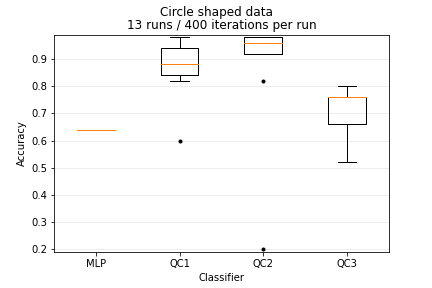
\includegraphics{Appendices/chapter_5/2qubits_3layers_Circle_shaped_data_13runs_400.png}
            }
        \end{subfigure}
        \begin{subfigure}{1.0\textwidth}
            \centering
            \scalebox{0.45}{
                 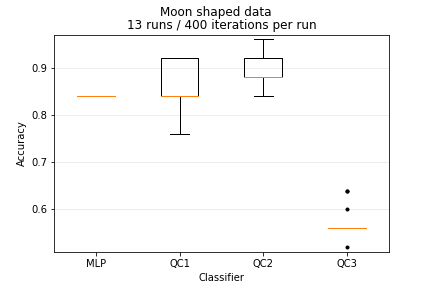
\includegraphics{Appendices/chapter_5/2qubits_3layers_Moon_shaped_data_13runs_400.png}
            }
        \end{subfigure}
        \caption{Accuracy box plots: \textbf{400 iterations} for all classifiers using \textbf{two qubit quantum circuits with 3 layers}.\\ \textbf{MLP}, \textbf{QC1}, \textbf{QC2} and \textbf{QC3} are referring to \textbf{Multi-layer Perceptron classifier}, \textbf{Quantum Circuit classifier 1}, \textbf{Quantum Circuit classifier 2} and \textbf{Quantum Circuit classifier 3} in figure \ref{fig:2Qubit3LayersClassifiers_400Iterations} accordingly.}
        \label{fig:2Qubit3LayersClassifiers_400Iterations_boxplot}
    \end{subfigure}
\end{figure}

\clearpage
\section{Discussion}

\subsection{Single qubit classifiers}
\label{subsection:single_qubit_circuits_discussion}
Examining the single qubit classifier plots and comparing the quantum classifiers decision boundaries, it becomes obvious that the replacing of the $\mathrm{RY}$ gate in \textit{Quantum Circuit classifier 1} (\ref{fig:single_qubit_circuit_1}) with a $\mathrm{RX}$ gate in \textit{Quantum Circuit classifier 2} (\ref{fig:single_qubit_circuit_2}) for the feature $x_1$ enhanced the expressiveness of the \textit{Quantum Circuit classifier 2} in a mostly beneficial way, resulting in a higher score over nearly all iteration counts.

Another interesting observation is that the \textit{Quantum Circuit classifier 1} only consisting of $\mathrm{RY}$ and $\mathrm{RZ}$ gates can adapt the weights to more and more resemble the data, mostly increasing the score with higher iterations, but achieving this much slower than \textit{Quantum Circuit classifier 2}. 

Comparing the linearly separable data (\textit{Row 1} of figure \ref{fig:SingleQubitClassifiers_50Iterations}) between the \textit{Multi-layer Perceptron classifier} and \textit{Quantum Circuit classifier 2} with only 50 iterations, the \textit{Quantum Circuit classifier 2} outperforms the \textit{Multi-layer Perceptron classifier}, but the \textit{Multi-layer Perceptron classifier} can keep up again and over perform with more iterations as seen in figures \ref{fig:SingleQubitClassifiers_200Iterations} and \ref{fig:SingleQubitClassifiers_400Iterations}, at least for the linearly separable data.

By comparing the contour plots of figure \ref{fig:SingleQubitClassifiers_400Iterations}, one can see that all the quantum circuit classifiers behave almost like the \textit{Multi-layer Perceptron classifier}. The accuracies in figure \ref{fig:SingleQubitClassifiers_400Iterations_boxplot} are also very close, except for \textit{Quantum Circuit classifier 1} with the moon shaped dataset in \textit{Row 3}.

One of the most important observations, however, is that the quantum circuit classifiers cannot produce smaller angles in all the contour plots, indicating that either the gates used are incorrect or their number is insufficient. Although smaller angles are needed to achieve a higher score when data points start to overlap, this can also have a negative impact on generalization like overfitting.

\subsection{Two qubit classifiers}
\label{subsection:two_qubit_circuits_discussion}
Interestingly, the accuracy for the two qubit classifiers (figures \ref{fig:2QubitClassifiers_50Iterations_boxplot}, \ref{fig:2QubitClassifiers_200Iterations_boxplot}, \ref{fig:2QubitClassifiers_400Iterations_boxplot}) is not better than the single qubit classifiers (figures \ref{fig:SingleQubitClassifiers_50Iterations_boxplot}, \ref{fig:SingleQubitClassifiers_200Iterations_boxplot}, \ref{fig:SingleQubitClassifiers_400Iterations_boxplot}) even though two more quantum gates were used e.g. the $\mathrm{CX}$ and the Hadamard ($\mathrm{H}$) see circuits \ref{fig:two_qubit_circuit_1}, \ref{fig:two_qubit_circuit_2}, \ref{fig:two_qubit_circuit_3}. For the circular (\textit{Row 2}) and moon shaped (\textit{Row 2}) datasets the accuracy is even worse compared to the single qubit classifiers, which is also evident in the contour plots because these do not show a significantly higher expression strength. Only the linear data set has a similarly high and slightly more stable accuracy. 

As with the single qubit classifiers, comparing the linearly separable data (\textit{Row 1} of figure \ref{fig:2Qubit3LayersClassifiers_50Iterations}) between the \textit{Multi-layer Perceptron classifier} and all of the two qubit classifiers with only 50 iterations, all two qubit classifiers outperform the \textit{Multi-layer Perceptron classifier}, but the \textit{Multi-layer Perceptron classifier} can keep up again and slightly over perform with more iterations as seen in figures \ref{fig:2QubitClassifiers_200Iterations} and \ref{fig:2Qubit3LayersClassifiers_400Iterations}.

\textit{Quantum Circuit classifier 3} can only perform a linear classification and is very limited in its expressiveness, as the contour plots (figures \ref{fig:2QubitClassifiers_50Iterations}, \ref{fig:2QubitClassifiers_200Iterations}, \ref{fig:2QubitClassifiers_400Iterations}) indicate. The accuracy for the non-linear separable data sets (figures \ref{fig:2QubitClassifiers_50Iterations_boxplot}, \ref{fig:2QubitClassifiers_200Iterations_boxplot}, \ref{fig:2QubitClassifiers_400Iterations_boxplot}) is correspondingly poor.

The \textit{Multi-layer Perceptron classifier} leaves all two qubit classifiers behind regarding accuracy for the moon shaped data sets for all iteration counts (figures \ref{fig:2Qubit3LayersClassifiers_50Iterations_boxplot}, \ref{fig:2Qubit3LayersClassifiers_200Iterations_boxplot}, \ref{fig:2Qubit3LayersClassifiers_400Iterations_boxplot}). 

\subsection{Two qubit classifiers with 3 layers}
\label{subsection:two_qubit_3layer_circuits_discussion}

When inspecting the contour plots in figures \ref{fig:2Qubit3LayersClassifiers_50Iterations}, \ref{fig:2Qubit3LayersClassifiers_200Iterations} and \ref{fig:2Qubit3LayersClassifiers_400Iterations}, it is obvious that the contours can now take on much smaller angles or fields and the expressiveness has increased a lot even with a few iterations.

The accuracy advantage over the \textit{Multi-layer Perceptron classifier} at 50 iterations - observed with the single qubit \ref{subsection:single_qubit_circuits_discussion} and two qubit classifiers \ref{subsection:two_qubit_circuits_discussion} - has significantly decreased for the linearly separable dataset \textit{Row 1}, which makes sense since now a lot more weights have to be trained and the features are additionally encoded twice resulting in more complex computation of the quantum circuit (see figures \ref{fig:2Qubit3LayersClassifiers_50Iterations_boxplot}, \ref{fig:2Qubit3LayersClassifiers_200Iterations_boxplot}, \ref{fig:2Qubit3LayersClassifiers_400Iterations_boxplot}). 

\textit{Quantum Circuit classifier 3} behaves no longer only "linearly" and can improve with higher iteration numbers its expression strength, even if only slowly. \textit{Quantum Circuit classifier 1} and \textit{Quantum Circuit classifier 2} show promising contours and accuracies with three layers starting at 100 iterations (see figures \ref{fig:2Qubit3LayersClassifiers_50Iterations}, \ref{fig:2Qubit3LayersClassifiers_200Iterations}, \ref{fig:2Qubit3LayersClassifiers_400Iterations}). All three circuits tend to achieve higher accuracy than the \textit{Multi-layer Perceptron classifier} in the circular and moon-shaped data sets starting at 100 iterations, except for \textit{Quantum Circuit classifier 3} on the moon-shaped data set (see figures \ref{fig:2Qubit3LayersClassifiers_50Iterations_boxplot}, \ref{fig:2Qubit3LayersClassifiers_200Iterations_boxplot}, \ref{fig:2Qubit3LayersClassifiers_400Iterations_boxplot}). 

\section{Conclusion}
The experiments with different quantum classifier circuits using contour and box plots in comparison with a classical \textit{Multi-layer Perceptron classifier} showed that small gates changes - for example a rotation around another axis - can result in a very different decision boundary improving/decreasing the accuracy or can lead to slower/faster adaption of the decision boundary when trained.

Not only can single qubit classifiers perform well on certain data sets, they can also be more accurate than two qubit classifiers, depending on the data set complexity and the gates used. A big advantage are the quantum classifier circuits with multiple layers that have more weights and gates and thus a larger expression strength with smaller angles and fields that can adapt much better to more difficult datasets and this at an iteration count where the accuracy of the \textit{Multi-layer Perceptron classifier} is not nearly sufficient.

We cannot say how well the quantum classifier circuits used in the above experiments (\ref{subsection:single_qubit_circuits}, \ref{subsection:two_qubit_circuits} and \ref{subsection:two_qubit_circuits_3layers}) would perform in a real quantum computer given the accuracy, since we could only use quantum computer simulators due to time constraints. The accuracy of the different runs with the optimal simulator still varies enormously, in contrast to the \textit{Multi-layer Perceptron classifier}. This leads to the fact that runs have to be performed several times because an above-average bad/good run can occur more often.

It certainly needs more experiments and mathematical analysis of the quantum classifier circuits to be more precise. However, we advise using the contour plots as an additional tool to visually estimate the expression strength and adaptation to the data set for the used quantum circuit in the context of the training.
 
% Chapter 2

\chapter{Quantum Operations} % Main chapter title

\label{Chapter2}

\section{Basic operations}
\label{chapter:basic_opterations}

Before creating a quantum circuit, a basic understanding of quantum operations and gates is needed. Comparable to the classical bit, qubits are the more powerful quantum equivalent. Whilst classical bits can only assume a state of $1$ and $0$, a qubit can be $1$,$0$ or anything in between. The state of a single, non-entangled qubit can be visualized with the Bloch sphere\cite{bloch_nuclear_induction}. Figure \ref{fig:circuit_empty} shows a simple circuit containing one qubit, annotated with $q_0$, and figure \ref{fig:circuit_empty_bloch_sphere} shows the Bloch sphere for it.

\todo{Explain all gates, what does it and where is it used and why}

\begin{figure}[!h]
    \centering
    \scalebox{1.0}{
        \Qcircuit @C=1.0em @R=1.0em @!R { 
            \nghost{ {q}_{0} :  } & \lstick{ {q}_{0} :  } & \qw & \qw\\ 
        }
    }
    \caption{Empty single qubit circuit}
    \label{fig:circuit_empty}
\end{figure}

\begin{figure}[!h]
    \centering
    \scalebox{0.3}{
        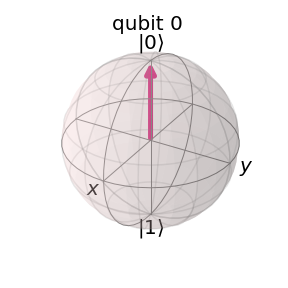
\includegraphics{Appendices/chapter_2/basic_bloch_sphere.png}
    }
    \caption{State vector on bloch sphere}
    \label{fig:circuit_empty_bloch_sphere}
\end{figure}

The visible arrow shows the current state, which lies directly on the $z$ axis. This state is described as a vector in equation \ref{equation:single_qubit_zero_state}.

\begin{equation}
    \ket{0} = \begin{pmatrix}1 \\ 0\end{pmatrix}
    \label{equation:single_qubit_zero_state}
\end{equation}

The classical NOT gate, that inverts the state of a chosen bit, also exists as a quantum gate. The matrix definition of the Pauli $\mathrm{X}$ gate is represented in figure \ref{fig:matrix_pauli_x}. When applying it to a qubit, a multiplication of the state vector of $q_0$ and the matrix $\mathrm{X}$ results in the inverted state $\ket{1}$, as demonstrated in equation \ref{equation:pauli_x_example}. The circuit for this example is shown in figure \ref{fig:circuit_negated_empty}. Figure \ref{fig:circuit_negated_empty_bloch_sphere} shows that our state now points in the opposite direction when compare to figure \ref{fig:circuit_empty_bloch_sphere}.

\begin{figure}
    \centering
    $\mathrm{X} = \begin{pmatrix}
        0 & 1 \\
        1 & 0
    \end{pmatrix}$
    \caption{Pauli X gate matrix}
    \label{fig:matrix_pauli_x}
\end{figure}

\begin{figure}[!h]
    \centering
    \scalebox{1.0}{
        \Qcircuit @C=1.0em @R=1.0em @!R { 
            \nghost{ {q}_{0} :  } & \lstick{ {q}_{0} :  } & \gate{\mathrm{X}} & \qw & \qw\\ 
        }
    }
    \caption{Negated single qubit circuit}
    \label{fig:circuit_negated_empty}
\end{figure}

\begin{figure}[!h]
    \centering
    \scalebox{0.3}{
        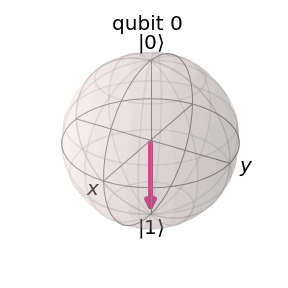
\includegraphics{Appendices/chapter_2/negated_bloch_sphere.png}
    }
    \caption{Negated state vector on bloch sphere}
    \label{fig:circuit_negated_empty_bloch_sphere}
\end{figure}

\begin{equation}
    \centering
    \begin{split}
        \mathrm{X}\ket{0} =\ \begin{pmatrix} 0 & 1 \\ 1 & 0 \end{pmatrix}\begin{pmatrix}1 \\ 0\end{pmatrix} =\ \begin{pmatrix}0 \\ 1\end{pmatrix} =\ \ket{1}
    \end{split}
    \label{equation:pauli_x_example}
\end{equation}

Superpositions are any state that is neither $\ket{0}$ and $\ket{1}$, but a combination of both. Such a state is defined as $\alpha\ket{0} + \beta\ket{1}$, where the quadratic value of $\alpha$ and $\beta$ corresponds to the probability of the given state, and there for $\alpha^2 + \beta^2 = 1$. When building quantum circuits, the Hadamard\cite{qiskit_hgate_nodate} gate can be used to put a qubit in an \emph{equal}, that is equal probability for $\ket{0}$ and $\ket{1}$, superposition. Figure \ref{fig:matrix_hadamard} shows the matrix definition of the Hadamard gate, figure \ref{fig:circuit_hadamard} a simple single qubit circuit with the Hadamard gate, and equation \ref{equation:hadamard_example} the calculation of said circuit. The Bloch sphere in figure \ref{fig:circuit_hadamard_bloch_sphere} shows the attained superposition, which is orthogonal to the $Z$ axis.

\begin{figure}[!h]
    \centering
    $\mathrm{H} = \frac{1}{\sqrt{2}}\begin{pmatrix}1 & 1 \\1 & -1\end{pmatrix}$
    \caption{Hadamard gate matrix}
    \label{fig:matrix_hadamard}
\end{figure}

\begin{equation}
    \centering
    \begin{split}
        \mathrm{H}\ket{0} =\ \frac{1}{\sqrt{2}}\begin{pmatrix}1 & 1 \\1 & -1\end{pmatrix}\begin{pmatrix}1 \\ 0\end{pmatrix} =\ \frac{\ket{0} + \ket{1}}{\sqrt{2}} =\ \frac{1}{\sqrt{2}}\ket{0} + \frac{1}{\sqrt{2}}\ket{1}
    \end{split}
    \label{equation:hadamard_example}
\end{equation}


\begin{figure}[!h]
    \centering
    \scalebox{1.0}{
        \Qcircuit @C=1.0em @R=1.0em @!R { 
            \nghost{ {q}_{0} :  } & \lstick{ {q}_{0} :  } & \gate{\mathrm{H}} & \qw & \qw\\ 
        }
    }
    \caption{Circuit with Hadamard gate}
    \label{fig:circuit_hadamard}
\end{figure}

\begin{figure}[!h]
    \centering
    \scalebox{0.3}{
        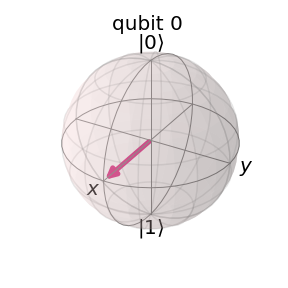
\includegraphics{Appendices/chapter_2/hadamard_bloch_sphere.png}
    }
    \caption{Superposition state on bloch sphere}
    \label{fig:circuit_hadamard_bloch_sphere}
\end{figure}

\section{Rotations}
\label{chapter:rotations}

As seen in chapter \ref{chapter:basic_opterations}, quantum gates apply rotations to the state inside the Bloch sphere. There exist parametrizable, rotational gates that rotate the state around a given axis, by the supplied value. One of those gates is the $\mathrm{RY}(\theta)$ gate\cite{qiskit_rygate_nodate}. The $\mathrm{RY}$ gate is constructed from the Pauli $\mathrm{Y}$ gate as shown in equation \ref{equation:pauli_y_to_ry}. Note that the resulting power series is equal to the ones defined for $\cos$ and $\sin$ in equation \ref{equation:power_series_sin_cos}\cite{lars_complex_1978}. As measurements in a quantum circuit are, to put it simply, collapsing the state vector onto the $Z$ axis\cite{feynman_feynman_1965}, rotation around the $Y$ axis have a direct impact on the probabilities of a measurement.

\begin{equation}
    \begin{split}
        \mathrm{RY}(\theta) &=\ e^{-i\frac{\theta}{2}\mathrm{Y}} =\ e^{\frac{-i\theta}{2}\begin{pmatrix} 0 & -i \\ i & 0 \end{pmatrix}} \\
        \mathrm{Y}' &=\ -i\frac{\theta}{2}\mathrm{Y} =\ \begin{pmatrix}
                                                         0 & \frac{-\theta}{2}\\
                                                         \frac{\theta}{2} & 0\\
                                                    \end{pmatrix} \\
        e^{\mathrm{Y}'} &=\ I^{2\times2} + \mathrm{Y}' + \frac{\mathrm{Y}'^2}{2!} + \frac{\mathrm{Y}'^3}{3!} + \frac{\mathrm{Y}'^4}{4!} + \cdot\cdot\cdot \\
        \mathrm{RY}(\theta) &=\ \begin{pmatrix}
         1 - \frac{\theta^2}{8} + \frac{\theta^4}{384} + \cdot\cdot\cdot & - \frac{\theta}{2} + \frac{\theta^3}{48} - \frac{\theta^5}{3840} + \cdot\cdot\cdot\\
         \frac{\theta}{2} - \frac{\theta^3}{48} + \frac{\theta^5}{3840} + \cdot\cdot\cdot & 1 - \frac{\theta^2}{8} + \frac{\theta^4}{384} + \cdot\cdot\cdot \\
         \end{pmatrix}\\ &=\ \begin{pmatrix}
        \cos{\frac{\theta}{2}} & -\sin{\frac{\theta}{2}} \\
        \sin{\frac{\theta}{2}} & \cos{\frac{\theta}{2}}
    \end{pmatrix}
    \end{split}
    \label{equation:pauli_y_to_ry}
\end{equation}

\begin{equation}
    \begin{split}
        \cos(x) &=\ 1 - \frac{x^2}{2!} + \frac{x^4}{4!} - \frac{x^6}{6!} + \cdot\cdot\cdot \\
        \sin(x) &= x - \frac{x^3}{3!} + \frac{x^5}{5!} - \frac{x^7}{7!} + \cdot\cdot\cdot
    \end{split}
    \label{equation:power_series_sin_cos}
\end{equation}

\begin{figure}[!h]
    \centering
    \scalebox{1.0}{
        \Qcircuit @C=1.0em @R=1.0em @!R { 
            \nghost{ {q}_{0} :  } & \lstick{ {q}_{0} :  } & \gate{\mathrm{R_Y}\,(\frac{\pi}{2})} & \qw & \qw\\ 
        }
    }
    \caption{Circuit with RY gate parameterized to $\frac{\pi}{2}$}
    \label{fig:circuit_ry}
\end{figure}

\begin{figure}[!h]
    \centering
    \scalebox{0.3}{
        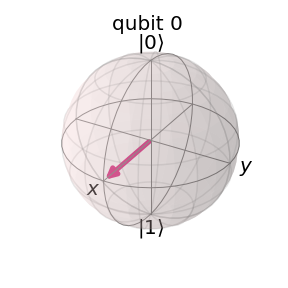
\includegraphics{Appendices/chapter_2/halfpi_yrotation_bloch_sphere.png}
    }
    \caption{Superposition state on Bloch sphere using RY gate}
    \label{fig:ry_bloch_sphere}
\end{figure}

\begin{figure}[!h]
    \centering
    \scalebox{0.5}{
        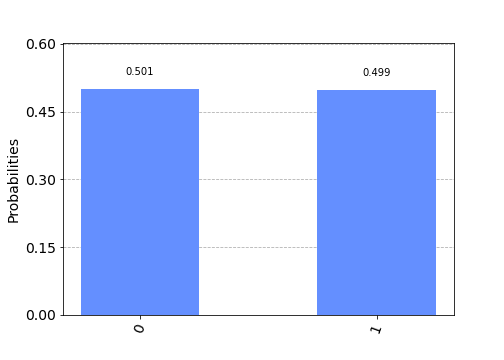
\includegraphics{Appendices/chapter_2/halfpi_yrotation_histogram.png}
    }
    \caption{Histogram of measurements done on circuit \ref{fig:circuit_ry}}
    \label{fig:histogram_ry}
\end{figure}

Quantum circuits with more than one qubit can use entanglement of both for advanced unitary operations. When entangling two qubits together, one has to start with calculating the tensor product of their state vectors. For circuit \ref{fig:circuit_double_hadamard}, the calculations are outlined in equation \ref{equation:two_hadamard_example}.

\begin{figure}[!h]
    \centering
    \scalebox{1.0}{
        \Qcircuit @C=1.0em @R=1.0em @!R { 
            \nghost{ {q}_{0} :  } & \lstick{ {q}_{0} :  } & \gate{\mathrm{H}} & \qw & \qw\\ 
            \nghost{ {q}_{1} :  } & \lstick{ {q}_{1} :  } & \gate{\mathrm{H}} & \qw & \qw\\ 
        }
    }
    \caption{Circuit with two Hadamard gates}
    \label{fig:circuit_double_hadamard}
\end{figure}

\begin{equation}
    \centering
    \begin{split}
        \mathrm{H}\ket{0} &=\ \frac{1}{\sqrt{2}}\begin{pmatrix}1 & 1 \\1 & -1\end{pmatrix}\begin{pmatrix}1 \\ 0\end{pmatrix} =\ \frac{\ket{0} + \ket{1}}{\sqrt{2}} \\
        \vec{s} &= \begin{pmatrix}\frac{1}{\sqrt{2}}\\\frac{1}{\sqrt{2}}\end{pmatrix} \otimes \begin{pmatrix}\frac{1}{\sqrt{2}}\\\frac{1}{\sqrt{2}}\end{pmatrix} = \begin{pmatrix}
            \frac{1}{2}\\\frac{1}{2}\\\frac{1}{2}\\\frac{1}{2}
        \end{pmatrix}
    \end{split}
    \label{equation:two_hadamard_example}
\end{equation}

\newpage
Quantum gates can be of any size and use as many qubits as they're designed for. Gates such as $\mathrm{CY}$\cite{qiskit_cygate_nodate}, $\mathrm{CX}$\cite{qiskit_cxgate_nodate} and $\mathrm{CZ}$\cite{qiskit_czgate_nodate} cover two qubits, of which one is a \emph{control} qubit. Depending on its state, the rotation is then applied to the second qubit. Figures \ref{fig:cy_entanglement}, \ref{fig:cx_entanglement} and \ref{fig:cz_entanglement} show the circuit design and the corresponding equations \ref{equation:cy_entanglement}, \ref{equation:cx_entanglement} and \ref{equation:cz_entanglement} show the behaviour of the state vector when entanglement is applied.

%--------------------------------

\begin{figure}[!h]
    \centering
    \scalebox{1.0}{
        \Qcircuit @C=1.0em @R=1.0em @!R { 
            \nghost{ {q}_{0} :  } & \lstick{ {q}_{0} :  } & \gate{\mathrm{H}} & \ctrl{1} & \qw & \qw\\
            \nghost{ {q}_{1} :  } & \lstick{ {q}_{1} :  } & \gate{\mathrm{H}} & \gate{\mathrm{Y}} & \qw & \qw\\
        }
    }
    \caption{Circuit entangled with a $\mathrm{CY}$ gate}
    \label{fig:cy_entanglement}
\end{figure}


\begin{equation}
    \centering
    \begin{split}
        \vec{s}_{\mathrm{CY}} &=\ \mathrm{CY}\begin{pmatrix}
            \frac{1}{2}\\\frac{1}{2}\\\frac{1}{2}\\\frac{1}{2}
        \end{pmatrix} =\  \begin{pmatrix}
        1 & 0 & 0 & 0 \\
        0 & 0 & 0 & -i \\
        0 & 0 & 1 & 0 \\
        0 & i & 0 & 0
    \end{pmatrix}\begin{pmatrix}
            \frac{1}{2}\\\frac{1}{2}\\\frac{1}{2}\\\frac{1}{2}
        \end{pmatrix} \\
        \vec{s}_{\mathrm{CY}} &= \begin{pmatrix}
            \frac{1}{2}\\\frac{-i}{2}\\\frac{1}{2}\\\frac{i}{2}
        \end{pmatrix}
    \end{split}
    \label{equation:cy_entanglement}
\end{equation}

%---------------------------------------

\begin{figure}[!h]
    \centering
    \scalebox{1.0}{
        \Qcircuit @C=1.0em @R=1.0em @!R { 
            \nghost{ {q}_{0} :  } & \lstick{ {q}_{0} :  } & \gate{\mathrm{H}} & \ctrl{1} & \qw & \qw\\
            \nghost{ {q}_{1} :  } & \lstick{ {q}_{1} :  } & \gate{\mathrm{H}} & \gate{\mathrm{X}} & \qw & \qw\\
        }
    }
    \caption{Circuit entangled with a $\mathrm{CX}$ gate}
    \label{fig:cx_entanglement}
\end{figure}

\begin{equation}
    \centering
    \begin{split}
        \vec{s}_{\mathrm{CX}} &=\ \mathrm{CX}\begin{pmatrix}
            \frac{1}{2}\\\frac{1}{2}\\\frac{1}{2}\\\frac{1}{2}
        \end{pmatrix} =\  \begin{pmatrix}
        1 & 0 & 0 & 0 \\
        0 & 0 & 0 & 1 \\
        0 & 0 & 1 & 0 \\
        0 & 1 & 0 & 0
    \end{pmatrix}\begin{pmatrix}
            \frac{1}{2}\\\frac{1}{2}\\\frac{1}{2}\\\frac{1}{2}
        \end{pmatrix} \\
        \vec{s}_{\mathrm{CX}} &= \begin{pmatrix}
            \frac{1}{2}\\\frac{1}{2}\\\frac{1}{2}\\\frac{1}{2}
        \end{pmatrix}
    \end{split}
    \label{equation:cx_entanglement}
\end{equation}

%-----------------------------------

\begin{figure}[!h]
    \centering
    \scalebox{1.0}{
        \Qcircuit @C=1.0em @R=1.0em @!R {
            \nghost{ {q}_{0} :  } & \lstick{ {q}_{0} :  } & \gate{\mathrm{H}} & \ctrl{1} & \qw & \qw\\
            \nghost{ {q}_{1} :  } & \lstick{ {q}_{1} :  } & \gate{\mathrm{H}} & \control\qw & \qw & \qw\\
        }
    }
    \caption{Circuit entangled with a $\mathrm{CZ}$ gate}
    \label{fig:cz_entanglement}
\end{figure}

\begin{equation}
    \centering
    \begin{split}
        \vec{s}_{\mathrm{CZ}} &=\ \mathrm{CZ}\begin{pmatrix}
            \frac{1}{2}\\\frac{1}{2}\\\frac{1}{2}\\\frac{1}{2}
        \end{pmatrix} =\  \begin{pmatrix}
        1 & 0 & 0 & 0 \\
        0 & 1 & 0 & 0 \\
        0 & 0 & 1 & 0 \\
        0 & 0 & 0 & -1
    \end{pmatrix}\begin{pmatrix}
            \frac{1}{2}\\\frac{1}{2}\\\frac{1}{2}\\\frac{1}{2}
        \end{pmatrix} \\
        \vec{s}_{\mathrm{CZ}} &= \begin{pmatrix}
            \frac{1}{2}\\\frac{1}{2}\\\frac{1}{2}\\\frac{-1}{2}
        \end{pmatrix}
    \end{split}
    \label{equation:cz_entanglement}
\end{equation}

\subsection{Measurement}
When measuring a quantum circuit, it always returns one of all the possible values. This is why when determining the result of a quantum circuit, multiples \emph{shots} are executed and from all the measured states the probabilities calculated. This also applies when calculating the probabilities. The statement in chapter \ref{chapter:basic_opterations} $\alpha^2 + \beta^2 = 1$ is a gross simplification of the process. To measure the probability of measuring $01$ in a two qubit circuit, we have to use a measurement matrix and surround it with our state $\ket{\psi}$\footnote{$\ket{\psi}$ stands for any arbitrary qubit state} and $\bra{\psi}$, which is the Hermitian transposition of $\ket{\psi}$. Equation \ref{equation:probability_calculation_example_1} demonstrates the steps needed to measure the probability of the state $01$ and equation \ref{equation:probability_calculation_example_2} for state $11$. Further calculations will use $M$ to resemble all four, single calculations and show them as a single vector.

\begin{equation}
    \centering
    \begin{split}
        \mathrm{P}_{Example} =\ \bra{\psi}M_2\ket{\psi} =\ \begin{pmatrix}
        \frac{-i}{\sqrt{2}} & \frac{i}{\sqrt{2}} & \frac{-i}{\sqrt{2}} & \frac{-i}{\sqrt{2}}
        \end{pmatrix}\begin{pmatrix}
        0 & 0 & 0 & 0 \\ 
        0 & 1 & 0 & 0 \\ 
        0 & 0 & 0 & 0\\ 
        0 & 0 & 0& 0\end{pmatrix}\begin{pmatrix}
        \frac{i}{\sqrt{2}} \\ \frac{-i}{\sqrt{2}} \\ \frac{i}{\sqrt{2}} \\ \frac{i}{\sqrt{2}}
        \end{pmatrix} =\ \frac{1}{2}
    \end{split}
    \label{equation:probability_calculation_example_1}
\end{equation}

\begin{equation}
    \centering
    \begin{split}
        \mathrm{P}_{Example} =\ \bra{\psi}M_4\ket{\psi} =\ \begin{pmatrix}
        \frac{-i}{\sqrt{2}} & \frac{i}{\sqrt{2}} & \frac{-i}{\sqrt{2}} & \frac{-i}{\sqrt{2}}
        \end{pmatrix}\begin{pmatrix}
        0 & 0 & 0 & 0 \\ 
        0 & 0 & 0 & 0 \\ 
        0 & 0 & 0 & 0\\ 
        0 & 0 & 0& 1\end{pmatrix}\begin{pmatrix}
        \frac{i}{\sqrt{2}} \\ \frac{-i}{\sqrt{2}} \\ \frac{i}{\sqrt{2}} \\ \frac{i}{\sqrt{2}}
        \end{pmatrix} =\ \frac{1}{2}
    \end{split}
    \label{equation:probability_calculation_example_2}
\end{equation}

As entanglement connects both qubits, any gate that is applied to one of those is directly applied to the other one. The circuit \ref{fig:circuit_cz_entangled_ry_gate} show a $\mathrm{RY}$ gate after the entanglement. To calculate this quantum circuit, an increase in dimensionality of the target gate is done. Equation \ref{equation:2_x_2_ry} demonstrates how the identity matrix is used on the $\mathrm{RY}$ gate.

 \begin{equation}
     \centering
     \begin{split}
        \mathrm{RY}(\theta)^{2\times2} =\ I^{2\times2}\otimes\mathrm{RY}(\theta) =\  \begin{pmatrix}
        \cos{\frac{\theta}{2}} & -\sin{\frac{\theta}{2}} & 0 & 0\\
        \sin{\frac{\theta}{2}} & \cos{\frac{\theta}{2}} & 0 & 0 \\
        0 & 0 & \cos{\frac{\theta}{2}} & -\sin{\frac{\theta}{2}}\\
        0 & 0 & \sin{\frac{\theta}{2}} & \cos{\frac{\theta}{2}}\\
    \end{pmatrix}\\
     \end{split}
     \label{equation:2_x_2_ry}
 \end{equation}

Equations \ref{equation:cz_entanglement_with_ry}, \ref{equation:cx_entanglement_with_ry} and \ref{equation:cz_entanglement_with_ry} show the calculations for each type of entanglement. The final measurement calculations for the respective variants are shown in equations \ref{equation:cz_entanglement_with_ry}, \ref{equation:cx_entanglement_with_ry} and \ref{equation:cy_entanglement_with_ry}.

\begin{figure}[!ht]
    \centering
    \scalebox{1.0}{
        \Qcircuit @C=1.0em @R=0.2em @!R { 
            \nghost{ {q}_{0} :  } & \lstick{ {q}_{0} :  } & \gate{\mathrm{H}} & \ctrl{1} & \gate{\mathrm{R_Y}\,(\frac{\pi}{4})} & \qw & \qw\\
            \nghost{ {q}_{1} :  } & \lstick{ {q}_{1} :  } & \gate{\mathrm{H}} & \control\qw & \qw & \qw & \qw\
            }
        }
    \caption{Circuit with $\mathrm{CZ}$ entanglement and $\mathrm{RY}$ gate}
    \label{fig:circuit_cz_entangled_ry_gate}
\end{figure}

\begin{equation}
    \centering
    \begin{split}
    \mathrm{RY}(\theta)^{2\times2}\vec{s}_{\mathrm{CZ}} &=\ \begin{pmatrix}
        \cos{\frac{\theta}{2}} & -\sin{\frac{\theta}{2}} & 0 & 0\\
        \sin{\frac{\theta}{2}} & \cos{\frac{\theta}{2}} & 0 & 0 \\
        0 & 0 & \cos{\frac{\theta}{2}} & -\sin{\frac{\theta}{2}}\\
        0 & 0 & \sin{\frac{\theta}{2}} & \cos{\frac{\theta}{2}}
    \end{pmatrix}\begin{pmatrix}
            \frac{1}{2}\\\frac{1}{2}\\\frac{1}{2}\\\frac{-1}{2}
        \end{pmatrix} \\
        \ket{\psi_{CZ}} &= \begin{pmatrix}
     0.2706\\
     0.65328\\
     0.65328\\
     -0.2706\\
     \end{pmatrix} \\
     \mathrm{P_{CZ}} &=\ \bra{\psi_{CZ}}M\ket{\psi_{CZ}} =\ \begin{pmatrix}
     0.073223\\
     0.42678\\
     0.42678\\
     0.073223\\
     \end{pmatrix}
    \end{split}
    \label{equation:cz_entanglement_with_ry}
\end{equation}

\begin{equation}
    \centering
    \begin{split}
         \mathrm{P_{CX}} &=\ \bra{\psi_{CX}}M\ket{\psi_{CX}} \rightarrow \begin{pmatrix}
         0.073223\\
         0.42678\\
         0.073223\\
         0.42678\\
     \end{pmatrix}
    \end{split}
    \label{equation:cx_entanglement_with_ry}
\end{equation}

\begin{equation}
    \centering
    \begin{split}
         \mathrm{P_{CY}} &=\ \bra{\psi_{CY}}M\ket{\psi_{CY}} \rightarrow \begin{pmatrix}
         0.25\\
         0.25\\
         0.25\\
         0.25\\
     \end{pmatrix}
    \end{split}
    \label{equation:cy_entanglement_with_ry}
\end{equation}

To assess the differences between the application of the rotation gate $\mathrm{RY}$ before the entanglement, circuit \ref{fig:circuit_ry_gate_cz_entangled} is calculated. The initial step to apply $\mathrm{RY}(\theta)$ to $q_0$, as seen in equation \ref{equation:hadamard_ry_before_entanglement}.

\begin{figure}[!ht]
    \centering
    \scalebox{1.0}{
        \Qcircuit @C=1.0em @R=0.2em @!R { 
	 	    \nghost{ {q}_{0} :  } & \lstick{ {q}_{0} :  } & \gate{\mathrm{H}} & \gate{\mathrm{R_Y}\,(\mathrm{\frac{\pi}{4}})} \barrier[0em]{1} & \qw & \ctrl{1} & \qw & \qw\\ 
	 	    \nghost{ {q}_{1} :  } & \lstick{ {q}_{1} :  } & \gate{\mathrm{H}} & \qw & \qw & \control\qw & \qw & \qw\\ 
	 	    \nghost{ {text} :  } & \lstick{  } & & &\ket{\psi_0} & & &\\ 
        }
    }
    \caption{Circuit with a $\mathrm{RY}$ gate and $\mathrm{CZ}$ entangled}
    \label{fig:circuit_ry_gate_cz_entangled}
\end{figure}

\begin{equation}
        \centering
    \begin{split}
          \ket{\psi_0} =\ \mathrm{RY}(\frac{\pi}{4})\mathrm{H}\ket{0} &=\ \begin{pmatrix}
        \cos{\frac{\pi}{8}} & -\sin{\frac{\pi}{8}} \\
        \sin{\frac{\pi}{8}} & \cos{\frac{\pi}{8}}
    \end{pmatrix}\begin{pmatrix}\frac{1}{\sqrt{2}}\\\frac{1}{\sqrt{2}}\end{pmatrix} \\
    \ket{\psi_0} &=\ \begin{pmatrix}
     0.38268\\
     0.92388\\
     \end{pmatrix}
    \end{split}
    \label{equation:hadamard_ry_before_entanglement}
\end{equation}

\begin{equation}
    \centering
    \begin{split}
    \ket{\psi_{CZ}} &=\ \mathrm{CZ}\ket{\psi_0}\otimes\mathrm{H}\ket{0} =\ \begin{pmatrix}
     0.2706\\
     0.2706\\
     0.65328\\
     0.65328\\
     \end{pmatrix} \\
         \mathrm{P_{CZ}} &=\ \bra{\psi_{CZ}}M\ket{\psi_{CZ}} \rightarrow \begin{pmatrix}
         0.073223\\
         0.073223\\
         0.42678\\
         0.42678\\
     \end{pmatrix}
    \end{split}
    \label{equation:h_ry_cz_entanglement}
\end{equation}

\begin{equation}
    \centering
    \begin{split}
    \ket{\psi_{CX}} &=\ \mathrm{CX}\ket{\psi_0}\otimes\mathrm{H}\ket{0} =\ \begin{pmatrix}
     0.2706\\
     0.2706\\
     0.65328\\
     0.65328\\
     \end{pmatrix} \\
    \mathrm{P_{CX}} &=\ \bra{\psi_{CX}}M\ket{\psi_{CX}} \rightarrow \begin{pmatrix}
     0.073223\\
     0.073223\\
     0.42678\\
     0.42678\\
     \end{pmatrix}
    \end{split}
    \label{equation:h_ry_cx_entanglement}
\end{equation}

\begin{equation}
    \centering
    \begin{split}
    \ket{\psi_{CY}} &=\ \mathrm{CY}\ket{\psi_0}\otimes\mathrm{H}\ket{0} =\ \begin{pmatrix}
     0.2706\\
     0-0.65328i\\
     0.65328\\
     0+0.2706i\\
     \end{pmatrix} \\
    \mathrm{P_{CY}} &=\ \bra{\psi_{CY}}M\ket{\psi_{CY}} \rightarrow \begin{pmatrix}
    0.0732\\
    0.4268\\
    0.4268\\
    0.0732\\
     \end{pmatrix}
    \end{split}
    \label{equation:h_ry_cy_entanglement}
\end{equation}

Whereas equation \ref{equation:cy_entanglement_with_ry} shows that when applying $\mathrm{RY}$ after the entanglement, it returns the states to their previous probabilities,  equation \ref{equation:h_ry_cy_entanglement} losses none of its operations. This indicates that applying the weights before the entanglement can result in a wider range of results.

%----------------------------------------------------------------------------------------
\clearpage
\section{Visual Comparison Between A Neural Network And Quantum Circuit}

To design the quantum equivalent to a neural net, a visual comparison is created and traced. Figure \ref{fig:comparison_neuron_feature_weight_quantum} contains an exemplary neural network, where each $\sum_i$ represents a single node. The highlighted paths are converted into their quantum counterparts. In an initial step, the input layer with features and weights is created. Equation \ref{equation:quantum_feature_weight} shows the mathematical operation that is executed on a single qubit.

\begin{figure}[!h]
\begin{subfigure}{.5\textwidth}
\centering
  \begin{tikzpicture}[shorten >=1pt,node distance=1.5cm,on grid,auto]
    	\node (0) {\colorbox{yellow}{$i_0$}};
    	\node (1) [below=of 0] {\colorbox{yellow}{$i_1$}};
    	\node (2) [below=of 1] {\colorbox{yellow}{$i_2$}};
    	\node (3) [below=of 2] {\colorbox{yellow}{$i_3$}};
    	\node (4) [right=of 0] {$\sum_0$};
    	\node (5) [right=of 3] {$\sum_1$};
    	\node (6) [right=of 4] {$\sum_2$};
    	\node (7) [right=of 5] {$\sum_3$};
    	\path[->]
    	(0) edge [preaction={draw,yellow,-,double=yellow,double distance=2\pgflinewidth,}] node {\colorbox{yellow}{$\omega_0$}} (4)
    	(1) edge [preaction={draw,yellow,-,double=yellow,double distance=2\pgflinewidth,},bend right=25] node {\colorbox{yellow}{$\omega_1$}} (4)
    	(2) edge [preaction={draw,yellow,-,double=yellow,double distance=2\pgflinewidth,},bend left=25] node {\colorbox{yellow}{$\omega_2$}} (5)
    	(3) edge [preaction={draw,yellow,-,double=yellow,double distance=2\pgflinewidth,}] node {\colorbox{yellow}{$\omega_3$}} (5)
    	(4) edge (6)
    	(4) edge (7)
    	(5) edge (7);
    \end{tikzpicture}
    \caption{Features with their corresponding weights}
\end{subfigure}
\begin{subfigure}{.5\textwidth}
\centering
    \scalebox{1.0}{
        \Qcircuit @C=1.0em @R=0.2em @!R { 
            \nghost{ {q}_{0} :  } & \lstick{ {q}_{0} :  } & \gate{\mathrm{R_Y}\, (\mathrm{i_0})} & \gate{\mathrm{R_Y}\,(\mathrm{w_0})} & \qw & \qw\\
            \nghost{ {q}_{1} :  } & \lstick{ {q}_{1} :  } & \gate{\mathrm{R_Y}\, (\mathrm{i_1})} & \gate{\mathrm{R_Y}\,(\mathrm{w_1})} & \qw & \qw\\
            \nghost{ {q}_{2} :  } & \lstick{ {q}_{2} :  } & \gate{\mathrm{R_Y}\, (\mathrm{i_2})} & \gate{\mathrm{R_Y}\,(\mathrm{w_2})} & \qw & \qw\\
            \nghost{ {q}_{3} :  } & \lstick{ {q}_{3} :  } & \gate{\mathrm{R_Y}\, (\mathrm{i_3})} & \gate{\mathrm{R_Y}\,(\mathrm{w_3})} & \qw & \qw\\
        }
    }
    \caption{Circuit with RY gates for input features and their weights}
\end{subfigure}%
\caption{Comparison of the feature$\cdot$weight component of a computation neuron and the quantum equivalent}
\label{fig:comparison_neuron_feature_weight_quantum}
\end{figure}

\begin{equation}
    \centering
    \begin{split}
        \mathrm{RY}(\omega_0)\mathrm{RY}(i_0)\ket{0} &=\ \begin{pmatrix}
        \cos{\frac{\omega_0}{2}} & -\sin{\frac{\omega_0}{2}} \\
        \sin{\frac{\omega_0}{2}} & \cos{\frac{\omega_0}{2}}
    \end{pmatrix}\begin{pmatrix}
        \cos{\frac{i_0}{2}} & -\sin{\frac{i_0}{2}} \\
        \sin{\frac{i_0}{2}} & \cos{\frac{i_0}{2}}
    \end{pmatrix} \begin{pmatrix}
        1 \\ 0
    \end{pmatrix}\\ \rightarrow q_0 &=\ \begin{pmatrix}
     \cos\frac{i_{0}}{2}\cos\frac{\omega_{0}}{2} - \sin\frac{i_{0}}{2}\sin\frac{\omega_{0}}{2}\\
     \cos\frac{i_{0}}{2}\sin\frac{\omega_{0}}{2} + \cos\frac{\omega_{0}}{2}\sin\frac{i_{0}}{2}\\
     \end{pmatrix}
    \end{split}
    \label{equation:quantum_feature_weight}
\end{equation}

It is important to note that whilst graphically they appear to do the same, the behaviour is quite different. Where the computational neuron performs classical multiplications, the quantum counterpart operates with rotations, as demonstrated in chapter \ref{chapter:rotations}. The \emph{probability} of a given state is, depending on the rotation, reinforced or weakened.\par

The next step is to rebuild the two partially connected nodes $\sum_0$ and $\sum_1$, as highlighted in figure \ref{fig:comparison_neuron_feature_weight_entanglement_quantum}. Note that we first have to increase the dimension of the state vector by calculating the tensor product of $q_0$ and $q_1$, as seen in equation \ref{equation:tensor_product_two_qubits}. The entanglement itself is calculated in equation \ref{equation:entanglement_calculation} using the $\mathrm{CZ}$ gate.

\clearpage

\begin{figure}[!h]
\begin{subfigure}{.5\textwidth}
\centering
  \begin{tikzpicture}[shorten >=1pt,node distance=1.5cm,on grid,auto]
    	\node (0) {$i_0$};
    	\node (1) [below=of 0] {$i_1$};
    	\node (2) [below=of 1] {$i_2$};
    	\node (3) [below=of 2] {$i_3$};
    	\node (4) [right=of 0] {\colorbox{yellow}{$\sum_0$}};
    	\node (5) [right=of 3] {\colorbox{yellow}{$\sum_1$}};
    	\node (6) [right=of 4] {$\sum_2$};
    	\node (7) [right=of 5] {$\sum_3$};
    	\path[->]
    	(0) edge node {$\omega_0$} (4)
    	(1) edge [bend right=25] node {$\omega_1$} (4)
    	(2) edge [bend left=25] node {$\omega_2$} (5)
    	(3) edge node {$\omega_3$} (5)
    	(4) edge (6)
    	(4) edge (7)
    	(5) edge (7);
    \end{tikzpicture}
    \caption{Features with their corresponding weights}
\end{subfigure}
\begin{subfigure}{.5\textwidth}
\centering
    \scalebox{1.0}{
    \Qcircuit @C=1.0em @R=0.2em @!R {
        \nghost{ {q}_{0} :  } & \lstick{ {q}_{0} :  } & \gate{\mathrm{R_Y}\,(\mathrm{i_0})} & \gate{\mathrm{R_Y}\,(\mathrm{w_0})} \barrier[0em]{1} & \qw & \ctrl{1} \barrier[0em]{1}& \qw & \qw\\ 
        \nghost{ {q}_{1} :  } & \lstick{ {q}_{1} :  } & \gate{\mathrm{R_Y}\,(\mathrm{i_1})} & \gate{\mathrm{R_Y}\,(\mathrm{w_1})} & \qw & \control\qw & \qw & \qw\\
        \nghost{} & \lstick{} & & & \ket{\psi_0}  & & \ket{\psi_1} &\\
        \nghost{ {q}_{2} :  } & \lstick{ {q}_{2} :  } & \gate{\mathrm{R_Y}\,(\mathrm{i_2})} & \gate{\mathrm{R_Y}\,(\mathrm{w_2})} & \ctrl{1} & \qw & \qw\\
        \nghost{ {q}_{3} :  } & \lstick{ {q}_{3} :  } & \gate{\mathrm{R_Y}\,(\mathrm{i_3})} & \gate{\mathrm{R_Y}\,(\mathrm{w_3})} & \control\qw & \qw & \qw\\
        }
    }
    \caption{Circuit with RY gates for input features and their weights}
\end{subfigure}%
\caption{Comparison of summation nodes and their quantum entanglement equivalent.}
\label{fig:comparison_neuron_feature_weight_entanglement_quantum}
\end{figure}


\begin{equation}
    \centering
    \begin{split}
        \ket{\psi_0} &=\ \mathrm{RY}(\omega_0)\mathrm{RY}(i_0) \otimes \mathrm{RY}(\omega_1)\mathrm{RY}(i_1) \\ 
        \ket{\psi_0} &=\ \begin{pmatrix}
            \cos\frac{i_{0}}{2}\cos\frac{\omega_{0}}{2} - \sin\frac{i_{0}}{2}\sin\frac{\omega_{0}}{2}\\
            \cos\frac{i_{0}}{2}\sin\frac{\omega_{0}}{2} + \cos\frac{\omega_{0}}{2}\sin\frac{i_{0}}{2}\\
        \end{pmatrix} \otimes 
        \begin{pmatrix}
            \cos\frac{i_{1}}{2}\cos\frac{\omega_{1}}{2} - \sin\frac{i_{1}}{2}\sin\frac{\omega_{1}}{2}\\
            \cos\frac{i_{1}}{2}\sin\frac{\omega_{1}}{2} + \cos\frac{\omega_{1}}{2}\sin\frac{i_{1}}{2}\\
        \end{pmatrix} \\
        \ket{\psi_0} &=\ \begin{pmatrix}
     (\cos\frac{i_{0}}{2}\cos\frac{\omega_{0}}{2} - \sin\frac{i_{0}}{2}\sin\frac{\omega_{0}}{2})(\cos\frac{i_{1}}{2}\cos\frac{\omega_{1}}{2} - \sin\frac{i_{1}}{2}\sin\frac{\omega_{1}}{2})\\
     (\cos\frac{i_{0}}{2}\cos\frac{\omega_{0}}{2} - \sin\frac{i_{0}}{2}\sin\frac{\omega_{0}}{2})(\cos\frac{i_{1}}{2}\sin\frac{\omega_{1}}{2} + \cos\frac{\omega_{1}}{2}\sin\frac{i_{1}}{2})\\
     (\cos\frac{i_{0}}{2}\sin\frac{\omega_{0}}{2} + \cos\frac{\omega_{0}}{2}\sin\frac{i_{0}}{2})(\cos\frac{i_{1}}{2}\cos\frac{\omega_{1}}{2} - \sin\frac{i_{1}}{2}\sin\frac{\omega_{1}}{2})\\
     (\cos\frac{i_{0}}{2}\sin\frac{\omega_{0}}{2} + \cos\frac{\omega_{0}}{2}\sin\frac{i_{0}}{2})(\cos\frac{i_{1}}{2}\sin\frac{\omega_{1}}{2} + \cos\frac{\omega_{1}}{2}\sin\frac{i_{1}}{2})\\
    \end{pmatrix}
    \end{split}
    \label{equation:tensor_product_two_qubits}
\end{equation}

\begin{equation}
    \centering
    \begin{split}
        \ket{\psi_1} &=\ CZ_{q_0,q_1}\ket{\psi_0} \\ 
        \ket{\psi_1} &=\ \begin{pmatrix}
        1 & 0 & 0 & 0 \\
        0 & 1 & 0 & 0 \\
        0 & 0 & 1 & 0 \\
        0 & 0 & 0 & -1
    \end{pmatrix}\begin{pmatrix}
     (\cos\frac{i_{0}}{2}\cos\frac{\omega_{0}}{2} - \sin\frac{i_{0}}{2}\sin\frac{\omega_{0}}{2})(\cos\frac{i_{1}}{2}\cos\frac{\omega_{1}}{2} - \sin\frac{i_{1}}{2}\sin\frac{\omega_{1}}{2})\\
     (\cos\frac{i_{0}}{2}\cos\frac{\omega_{0}}{2} - \sin\frac{i_{0}}{2}\sin\frac{\omega_{0}}{2})(\cos\frac{i_{1}}{2}\sin\frac{\omega_{1}}{2} + \cos\frac{\omega_{1}}{2}\sin\frac{i_{1}}{2})\\
     (\cos\frac{i_{0}}{2}\sin\frac{\omega_{0}}{2} + \cos\frac{\omega_{0}}{2}\sin\frac{i_{0}}{2})(\cos\frac{i_{1}}{2}\cos\frac{\omega_{1}}{2} - \sin\frac{i_{1}}{2}\sin\frac{\omega_{1}}{2})\\
     (\cos\frac{i_{0}}{2}\sin\frac{\omega_{0}}{2} + \cos\frac{\omega_{0}}{2}\sin\frac{i_{0}}{2})(\cos\frac{i_{1}}{2}\sin\frac{\omega_{1}}{2} + \cos\frac{\omega_{1}}{2}\sin\frac{i_{1}}{2})\\
    \end{pmatrix} \\
    \ket{\psi_1} &=\ \begin{pmatrix}
     (\cos\frac{i_{0}}{2}\cos\frac{\omega_{0}}{2} - \sin\frac{i_{0}}{2}\sin\frac{\omega_{0}}{2})(\cos\frac{i_{1}}{2}\cos\frac{\omega_{1}}{2} - \sin\frac{i_{1}}{2}\sin\frac{\omega_{1}}{2})\\
     (\cos\frac{i_{0}}{2}\cos\frac{\omega_{0}}{2} - \sin\frac{i_{0}}{2}\sin\frac{\omega_{0}}{2})(\cos\frac{i_{1}}{2}\sin\frac{\omega_{1}}{2} + \cos\frac{\omega_{1}}{2}\sin\frac{i_{1}}{2})\\
     (\cos\frac{i_{0}}{2}\sin\frac{\omega_{0}}{2} + \cos\frac{\omega_{0}}{2}\sin\frac{i_{0}}{2})(\cos\frac{i_{1}}{2}\cos\frac{\omega_{1}}{2} - \sin\frac{i_{1}}{2}\sin\frac{\omega_{1}}{2})\\
     -(\cos\frac{i_{0}}{2}\sin\frac{\omega_{0}}{2} + \cos\frac{\omega_{0}}{2}\sin\frac{i_{0}}{2})(\cos\frac{i_{1}}{2}\sin\frac{\omega_{1}}{2} + \cos\frac{\omega_{1}}{2}\sin\frac{i_{1}}{2})\\
     \end{pmatrix}
    \end{split}
    \label{equation:entanglement_calculation}
\end{equation}

\clearpage

At the end of the neural network, we have two more nodes, one of which is fully connected.

\begin{figure}[!h]
\begin{subfigure}{.5\textwidth}
\centering
  \begin{tikzpicture}[shorten >=1pt,node distance=1.5cm,on grid,auto]
    	\node (0) {$i_0$};
    	\node (1) [below=of 0] {$i_1$};
    	\node (2) [below=of 1] {$i_2$};
    	\node (3) [below=of 2] {$i_3$};
    	\node (4) [right=of 0] {$\sum_0$};
    	\node (5) [right=of 3] {$\sum_1$};
    	\node (6) [right=of 4] {$\sum_2$};
    	\node (7) [right=of 5] {$\sum_3$};
    	\path[->]
    	(0) edge node {$\omega_0$} (4)
    	(1) edge [bend right=25] node {$\omega_1$} (4)
    	(2) edge [bend left=25] node {$\omega_2$} (5)
    	(3) edge node {$\omega_3$} (5)
    	(4) edge (6)
    	(4) edge [preaction={draw,yellow,-,double=yellow,double distance=2\pgflinewidth,}] (7)
    	(5) edge (7);
    \end{tikzpicture}
    \caption{Features with their corresponding weights}
\end{subfigure}
\begin{subfigure}{.5\textwidth}
\centering
    \scalebox{1.0}{
    \Qcircuit @C=1.0em @R=0.2em @!R {
        \nghost{ {q}_{0} :  } & \lstick{ {q}_{0} :  } & \gate{\mathrm{R_Y}\,(\mathrm{i_0})} & \gate{\mathrm{R_Y}\,(\mathrm{w_0})} & \ctrl{1} & \qw &  \qw \barrier[0em]{3} & \qw & \qw\\ 
        \nghost{ {q}_{1} :  } & \lstick{ {q}_{1} :  } & \gate{\mathrm{R_Y}\,(\mathrm{i_1})} & \gate{\mathrm{R_Y}\,(\mathrm{w_1})} & \control\qw & \qw &  \ctrl{1} & \qw & \qw\\
        \nghost{ {q}_{2} :  } & \lstick{ {q}_{2} :  } & \gate{\mathrm{R_Y}\,(\mathrm{i_2})} & \gate{\mathrm{R_Y}\,(\mathrm{w_2})} & \ctrl{1} \barrier[0em]{1} & \qw  & \control\qw & \qw & \qw\\
        \nghost{ {q}_{3} :  } & \lstick{ {q}_{3} :  } & \gate{\mathrm{R_Y}\,(\mathrm{i_3})} & \gate{\mathrm{R_Y}\,(\mathrm{w_3})} & \control\qw & \qw &  \qw & \qw & \qw\\
        \nghost{ } & \lstick{ } & & & & \ket{\psi_2} & & \ket{\psi_3} & \\
        }
    }
    \caption{Circuit with RY gates for input features and their weights}
\end{subfigure}%
\caption{Comparison of final entanglement and output.}
\label{fig:comparison_measurment_layer}
\end{figure}

The shown neural network is designed to illustrate the core problem that entanglement brings. If we are to recreate the network shown in figure \ref{fig:comparison_measurment_layer}, we get full entanglement of all present qubits. Equation \ref{equation:full_entanglement_with_cz} shows the resulting state  $\ket{\psi_3}$. Figure \ref{fig:full_entanglement_networks} shows different neural network designs that lead to the same quantum circuit. Note that one could always measure a part of the circuit, and use that as an input for the next part that is represented in a different quantum circuit. This would allow us to recreate the given neural network fully, but increase complexity substantially, whilst also reducing the amount of transmitted information throughout the complete neural network.
    \begin{equation}
        \centering
        \resizebox{.9\hsize}{!}{
        $$
            \ket{\psi_3} =(I^{4\time4} \otimes CZ)(\ket{\psi_1} \otimes \ket{\psi_2}) =\ \begin{pmatrix}
         (\cos\frac{i_{0}}{2}\cos\frac{\omega_{0}}{2} - \sin\frac{i_{0}}{2}\sin\frac{\omega_{0}}{2})(\cos\frac{i_{1}}{2}\cos\frac{\omega_{1}}{2} - \sin\frac{i_{1}}{2}\sin\frac{\omega_{1}}{2})(\cos\frac{i_{2}}{2}\cos\frac{\omega_{2}}{2} - \sin\frac{i_{2}}{2}\sin\frac{\omega_{2}}{2})(\cos\frac{i_{3}}{2}\cos\frac{\omega_{3}}{2} - \sin\frac{i_{3}}{2}\sin\frac{\omega_{3}}{2})\\
         (\cos\frac{i_{0}}{2}\cos\frac{\omega_{0}}{2} - \sin\frac{i_{0}}{2}\sin\frac{\omega_{0}}{2})(\cos\frac{i_{1}}{2}\cos\frac{\omega_{1}}{2} - \sin\frac{i_{1}}{2}\sin\frac{\omega_{1}}{2})(\cos\frac{i_{2}}{2}\cos\frac{\omega_{2}}{2} - \sin\frac{i_{2}}{2}\sin\frac{\omega_{2}}{2})(\cos\frac{i_{3}}{2}\sin\frac{\omega_{3}}{2} + \cos\frac{\omega_{3}}{2}\sin\frac{i_{3}}{2})\\
         (\cos\frac{i_{0}}{2}\cos\frac{\omega_{0}}{2} - \sin\frac{i_{0}}{2}\sin\frac{\omega_{0}}{2})(\cos\frac{i_{1}}{2}\cos\frac{\omega_{1}}{2} - \sin\frac{i_{1}}{2}\sin\frac{\omega_{1}}{2})(\cos\frac{i_{2}}{2}\sin\frac{\omega_{2}}{2} + \cos\frac{\omega_{2}}{2}\sin\frac{i_{2}}{2})(\cos\frac{i_{3}}{2}\cos\frac{\omega_{3}}{2} - \sin\frac{i_{3}}{2}\sin\frac{\omega_{3}}{2})\\
         (\cos\frac{i_{0}}{2}\cos\frac{\omega_{0}}{2} - \sin\frac{i_{0}}{2}\sin\frac{\omega_{0}}{2})(\cos\frac{i_{1}}{2}\cos\frac{\omega_{1}}{2} - \sin\frac{i_{1}}{2}\sin\frac{\omega_{1}}{2})(\cos\frac{i_{2}}{2}\sin\frac{\omega_{2}}{2} + \cos\frac{\omega_{2}}{2}\sin\frac{i_{2}}{2})(\cos\frac{i_{3}}{2}\sin\frac{\omega_{3}}{2} + \cos\frac{\omega_{3}}{2}\sin\frac{i_{3}}{2})\\
         (\cos\frac{i_{0}}{2}\cos\frac{\omega_{0}}{2} - \sin\frac{i_{0}}{2}\sin\frac{\omega_{0}}{2})(\cos\frac{i_{1}}{2}\sin\frac{\omega_{1}}{2} + \cos\frac{\omega_{1}}{2}\sin\frac{i_{1}}{2})(\cos\frac{i_{2}}{2}\cos\frac{\omega_{2}}{2} - \sin\frac{i_{2}}{2}\sin\frac{\omega_{2}}{2})(\cos\frac{i_{3}}{2}\cos\frac{\omega_{3}}{2} - \sin\frac{i_{3}}{2}\sin\frac{\omega_{3}}{2})\\
         (\cos\frac{i_{0}}{2}\cos\frac{\omega_{0}}{2} - \sin\frac{i_{0}}{2}\sin\frac{\omega_{0}}{2})(\cos\frac{i_{1}}{2}\sin\frac{\omega_{1}}{2} + \cos\frac{\omega_{1}}{2}\sin\frac{i_{1}}{2})(\cos\frac{i_{2}}{2}\cos\frac{\omega_{2}}{2} - \sin\frac{i_{2}}{2}\sin\frac{\omega_{2}}{2})(\cos\frac{i_{3}}{2}\sin\frac{\omega_{3}}{2} + \cos\frac{\omega_{3}}{2}\sin\frac{i_{3}}{2})\\
         (\cos\frac{i_{0}}{2}\cos\frac{\omega_{0}}{2} - \sin\frac{i_{0}}{2}\sin\frac{\omega_{0}}{2})(\cos\frac{i_{1}}{2}\sin\frac{\omega_{1}}{2} + \cos\frac{\omega_{1}}{2}\sin\frac{i_{1}}{2})(\cos\frac{i_{2}}{2}\sin\frac{\omega_{2}}{2} + \cos\frac{\omega_{2}}{2}\sin\frac{i_{2}}{2})(\cos\frac{i_{3}}{2}\cos\frac{\omega_{3}}{2} - \sin\frac{i_{3}}{2}\sin\frac{\omega_{3}}{2})\\
         (\cos\frac{i_{0}}{2}\cos\frac{\omega_{0}}{2} - \sin\frac{i_{0}}{2}\sin\frac{\omega_{0}}{2})(\cos\frac{i_{1}}{2}\sin\frac{\omega_{1}}{2} + \cos\frac{\omega_{1}}{2}\sin\frac{i_{1}}{2})(\cos\frac{i_{2}}{2}\sin\frac{\omega_{2}}{2} + \cos\frac{\omega_{2}}{2}\sin\frac{i_{2}}{2})(\cos\frac{i_{3}}{2}\sin\frac{\omega_{3}}{2} + \cos\frac{\omega_{3}}{2}\sin\frac{i_{3}}{2})\\
         (\cos\frac{i_{0}}{2}\sin\frac{\omega_{0}}{2} + \cos\frac{\omega_{0}}{2}\sin\frac{i_{0}}{2})(\cos\frac{i_{1}}{2}\cos\frac{\omega_{1}}{2} - \sin\frac{i_{1}}{2}\sin\frac{\omega_{1}}{2})(\cos\frac{i_{2}}{2}\cos\frac{\omega_{2}}{2} - \sin\frac{i_{2}}{2}\sin\frac{\omega_{2}}{2})(\cos\frac{i_{3}}{2}\cos\frac{\omega_{3}}{2} - \sin\frac{i_{3}}{2}\sin\frac{\omega_{3}}{2})\\
         (\cos\frac{i_{0}}{2}\sin\frac{\omega_{0}}{2} + \cos\frac{\omega_{0}}{2}\sin\frac{i_{0}}{2})(\cos\frac{i_{1}}{2}\cos\frac{\omega_{1}}{2} - \sin\frac{i_{1}}{2}\sin\frac{\omega_{1}}{2})(\cos\frac{i_{2}}{2}\cos\frac{\omega_{2}}{2} - \sin\frac{i_{2}}{2}\sin\frac{\omega_{2}}{2})(\cos\frac{i_{3}}{2}\sin\frac{\omega_{3}}{2} + \cos\frac{\omega_{3}}{2}\sin\frac{i_{3}}{2})\\
         (\cos\frac{i_{0}}{2}\sin\frac{\omega_{0}}{2} + \cos\frac{\omega_{0}}{2}\sin\frac{i_{0}}{2})(\cos\frac{i_{1}}{2}\cos\frac{\omega_{1}}{2} - \sin\frac{i_{1}}{2}\sin\frac{\omega_{1}}{2})(\cos\frac{i_{2}}{2}\sin\frac{\omega_{2}}{2} + \cos\frac{\omega_{2}}{2}\sin\frac{i_{2}}{2})(\cos\frac{i_{3}}{2}\cos\frac{\omega_{3}}{2} - \sin\frac{i_{3}}{2}\sin\frac{\omega_{3}}{2})\\
         (\cos\frac{i_{0}}{2}\sin\frac{\omega_{0}}{2} + \cos\frac{\omega_{0}}{2}\sin\frac{i_{0}}{2})(\cos\frac{i_{1}}{2}\cos\frac{\omega_{1}}{2} - \sin\frac{i_{1}}{2}\sin\frac{\omega_{1}}{2})(\cos\frac{i_{2}}{2}\sin\frac{\omega_{2}}{2} + \cos\frac{\omega_{2}}{2}\sin\frac{i_{2}}{2})(\cos\frac{i_{3}}{2}\sin\frac{\omega_{3}}{2} + \cos\frac{\omega_{3}}{2}\sin\frac{i_{3}}{2})\\
         -(\cos\frac{i_{0}}{2}\sin\frac{\omega_{0}}{2} + \cos\frac{\omega_{0}}{2}\sin\frac{i_{0}}{2})(\cos\frac{i_{1}}{2}\sin\frac{\omega_{1}}{2} + \cos\frac{\omega_{1}}{2}\sin\frac{i_{1}}{2})(\cos\frac{i_{2}}{2}\cos\frac{\omega_{2}}{2} - \sin\frac{i_{2}}{2}\sin\frac{\omega_{2}}{2})(\cos\frac{i_{3}}{2}\cos\frac{\omega_{3}}{2} - \sin\frac{i_{3}}{2}\sin\frac{\omega_{3}}{2})\\
         -(\cos\frac{i_{0}}{2}\sin\frac{\omega_{0}}{2} + \cos\frac{\omega_{0}}{2}\sin\frac{i_{0}}{2})(\cos\frac{i_{1}}{2}\sin\frac{\omega_{1}}{2} + \cos\frac{\omega_{1}}{2}\sin\frac{i_{1}}{2})(\cos\frac{i_{2}}{2}\cos\frac{\omega_{2}}{2} - \sin\frac{i_{2}}{2}\sin\frac{\omega_{2}}{2})(\cos\frac{i_{3}}{2}\sin\frac{\omega_{3}}{2} + \cos\frac{\omega_{3}}{2}\sin\frac{i_{3}}{2})\\
         -(\cos\frac{i_{0}}{2}\sin\frac{\omega_{0}}{2} + \cos\frac{\omega_{0}}{2}\sin\frac{i_{0}}{2})(\cos\frac{i_{1}}{2}\sin\frac{\omega_{1}}{2} + \cos\frac{\omega_{1}}{2}\sin\frac{i_{1}}{2})(\cos\frac{i_{2}}{2}\sin\frac{\omega_{2}}{2} + \cos\frac{\omega_{2}}{2}\sin\frac{i_{2}}{2})(\cos\frac{i_{3}}{2}\cos\frac{\omega_{3}}{2} - \sin\frac{i_{3}}{2}\sin\frac{\omega_{3}}{2})\\
         -(\cos\frac{i_{0}}{2}\sin\frac{\omega_{0}}{2} + \cos\frac{\omega_{0}}{2}\sin\frac{i_{0}}{2})(\cos\frac{i_{1}}{2}\sin\frac{\omega_{1}}{2} + \cos\frac{\omega_{1}}{2}\sin\frac{i_{1}}{2})(\cos\frac{i_{2}}{2}\sin\frac{\omega_{2}}{2} + \cos\frac{\omega_{2}}{2}\sin\frac{i_{2}}{2})(\cos\frac{i_{3}}{2}\sin\frac{\omega_{3}}{2} + \cos\frac{\omega_{3}}{2}\sin\frac{i_{3}}{2})\\
         \end{pmatrix}
         $$
        }
        \label{equation:full_entanglement_with_cz}
    \end{equation}

\begin{figure}[!h]
\begin{subfigure}{.5\textwidth}
\centering
  \begin{tikzpicture}[shorten >=1pt,node distance=1.5cm,on grid,auto]
    	\node (0) {$i_0$};
    	\node (1) [below=of 0] {$i_1$};
    	\node (2) [below=of 1] {$i_2$};
    	\node (3) [below=of 2] {$i_3$};
    	\node (4) [right=of 0] {$\sum_0$};
    	\node (5) [right=of 3] {$\sum_1$};
    	\node (6) [right=of 4] {$\sum_2$};
    	\node (7) [right=of 5] {$\sum_3$};
    	\path[->]
    	(0) edge node {$\omega_0$} (4)
    	(1) edge [bend right=25] node {$\omega_1$} (4)
    	(2) edge [bend left=25] node {$\omega_2$} (5)
    	(3) edge node {$\omega_3$} (5)
    	(4) edge (6)
    	(5) edge (6)
    	(5) edge (7);
    \end{tikzpicture}
    \caption{Features with their corresponding weights}
\end{subfigure}
\begin{subfigure}{.5\textwidth}
\centering
  \begin{tikzpicture}[shorten >=1pt,node distance=1.5cm,on grid,auto]
    	\node (0) {$i_0$};
    	\node (1) [below=of 0] {$i_1$};
    	\node (2) [below=of 1] {$i_2$};
    	\node (3) [below=of 2] {$i_3$};
    	\node (4) [right=of 0] {$\sum_0$};
    	\node (5) [right=of 3] {$\sum_1$};
    	\node (6) [right=of 4] {$\sum_2$};
    	\node (7) [right=of 5] {$\sum_3$};
    	\path[->]
    	(0) edge node {$\omega_0$} (4)
    	(1) edge [bend right=25] node {$\omega_1$} (4)
    	(2) edge [bend left=25] node {$\omega_2$} (5)
    	(3) edge node {$\omega_3$} (5)
    	(4) edge (6)
    	(4) edge (7)
    	(5) edge (6)
    	(5) edge (7);
    \end{tikzpicture}
    \caption{Features with their corresponding weights}
\end{subfigure}%
\caption{Comparison of final entanglement and output.}
\label{fig:full_entanglement_networks}
\end{figure} 
% Chapter 3

\chapter{Quantum Classification Circuits} % Main chapter title

\label{Chapter3}

%----------------------------------------------------------------------------------------
\section{Quantum circuits}
\label{chapter:quantum_circuits}

Using the definitions from chapter \ref{chapter:quantum_embedding} and \ref{chapter:computational_neuron}, several quantum circuits are constructed for classification. \code{qiskit} offers a flexible approach for the gradient-based optimization of weights in a given circuit, as well as fine control of all components in the circuit and around the optimization. Based on the paper by Schuld et al. \cite{schuld_evaluating_2019}, we can optimize any given quantum circuit with a \code{NeuralNetworkClassifier}\cite{qiskit_neural_nodate}. The code to turn a single circuit into a classifier is shown in figure \ref{fig:code_qnn}. Note that the optimization itself is done in a classical fashion - only the classification is done with a quantum circuit. All calculations and classifications were done with the '\code{aer\_simulator}' from \code{qiskit}. The \code{NeuralNetworkClassifier} with \code{CircuitQNN} uses a measurement of all given qubits and the parity function \ref{fig:parity_function} to determine the label, where $n$ is the amount of different labels in the dataset.

\begin{figure}[!ht]
    \centering
    \begin{minted}{python}
    circuit_qnn = CircuitQNN(circuit=circuit,    
                         input_params=inputs,
                         weight_params=weights,
                         interpret=parity,
                         output_shape=output_shape,
                         quantum_instance=quantum_instance)

    nn_classifier = NeuralNetworkClassifier(neural_network=circuit_qnn, 
                                            optimizer=COBYLA())
    \end{minted}
    \caption{Python code to create a trainable neural network classifier from a quantum circuit}
    \label{fig:code_qnn}
\end{figure}

\begin{figure}[!ht]
    \centering
    \begin{minted}{python}
    def parity(x):
        return '{:b}'.format(x).count('1') % n
    \end{minted}
    \caption{Parity function to assign label after classification}
    \label{fig:parity_function}
\end{figure}

\clearpage

Figure \ref{fig:schematic_view_classical_and_quantum_circuit} is an overview of the training process. The features of a given dataset are preprocessed and then parameterized onto the state preparation part of the circuit. The weights are set from the optimizer, which also adapts them during training.

\begin{figure}[!h]
    \centering
    \scalebox{0.55}{
        \begin{tikzpicture}[
          roundnode/.style={circle, draw=black!60, fill=white!5, thick, minimum size=7mm},
          squarednode/.style={rectangle, draw=black!60, fill=white!5, thick, minimum size=10mm},
          optimizernode/.style={rectangle, draw=black!60, fill=white!5, thick, minimum size=25mm},
          quantumcircuit/.style={draw=blue, minimum height=3.5cm, minimum width=10cm, fill=white!5, label=below:{\color{blue}quantum\ circuit}},
        ]
            %Nodes
            \node[roundnode]        (dataset)        {Data};
            \node[squarednode]      (preprocess)     [right=of dataset] {Preprocessing};
            \node                   (point1)         [below=of preprocess] {};
            \node[quantumcircuit]   (quantumcircuit) [below right=of dataset]  {
                \Qcircuit @C=1em @R=.7em {
                    \lstick{\ket{0}} & \multigate{3}{state\ preparation} & \multigate{3}{model\ circuit} & \meter & \cw \\
                    \lstick{\ket{0}} & \ghost{state\ preparation} & \ghost{model\ circuit} & \meter & \cw \\
                    \cdots & \nghost{state\ preparation} & \nghost{model\ circuit} & \cdots &  \\
                    \lstick{\ket{0}} & \ghost{state\ preparation} & \ghost{model\ circuit} & \meter & \cw \gategroup{1}{5}{4}{5}{1.5em}{\}}
                }
            };
            \node[optimizernode]      (optimizer)     [right=of quantumcircuit] {Optimizer};
            % Lines
            \draw[->] (dataset.east) -- (preprocess.west);
            \draw[->] (quantumcircuit.east) -- (optimizer.west);
            \draw [->] (preprocess.south) -- ++(0,-.6) -- ++(+1.3,0) -| ++(0,-0.6);
            \draw [->] (optimizer.north) -- ++(0,+1.25) -- ++(-6.15,0) node[auto,midway,above] {updates} -| ++(0,-1);
        \end{tikzpicture}
    }
    \caption{Schematic view of classical and quantum circuit}
    \label{fig:schematic_view_classical_and_quantum_circuit}
\end{figure}

Figures \ref{fig:qc_ryrycryry} until \ref{fig:qc_ryryczry_2qbit} show the designs of the circuits used for the evaluation.


\begin{figure}[!ht]
    \centering
        \scalebox{0.5}{
        \Qcircuit @C=1.0em @R=0.2em @!R { 
            \ghost{ {q}_{0} :  } & \lstick{ {q}_{0} :  } & \gate{\mathrm{R_Y}\,(\mathrm{i_0})} & \gate{\mathrm{R_Y}\,(\mathrm{w_0})} & \ctrl{1} & \qw & \qw & \qw & \qw & \qw & \gate{\mathrm{R_Y}\,(\mathrm{w_13})} & \qw & \qw\\ 
            \ghost{ {q}_{1} :  } & \lstick{ {q}_{1} :  } & \gate{\mathrm{R_Y}\,(\mathrm{i_1})} & \qw & \gate{\mathrm{R_Y}\,(\mathrm{w_10})} & \gate{\mathrm{R_Y}\,(\mathrm{w_1})} & \ctrl{1} & \qw & \qw & \qw & \qw & \qw & \qw\\ 
            \ghost{ {q}_{2} :  } & \lstick{ {q}_{2} :  } & \gate{\mathrm{R_Y}\,(\mathrm{i_2})} & \qw & \qw & \qw & \gate{\mathrm{R_Y}\,(\mathrm{w_11})} & \gate{\mathrm{R_Y}\,(\mathrm{w_2})} & \ctrl{1} & \qw & \qw & \qw & \qw\\ 
            \ghost{ {q}_{3} :  } & \lstick{ {q}_{3} :  } & \gate{\mathrm{R_Y}\,(\mathrm{i_3})} & \qw & \qw & \qw & \qw & \qw & \gate{\mathrm{R_Y}\,(\mathrm{w_12})} & \gate{\mathrm{R_Y}\,(\mathrm{w_3})} & \ctrl{-3} & \qw & \qw\\
          }
        }
    \caption{Circuit 1 with $4$ qubits, $\mathrm{RY}$ gates before each entanglement, and entanglement with parameterized $\mathrm{CRY}$ gates}
    \label{fig:qc_ryrycryry}
\end{figure}

\begin{figure}[!ht]
    \centering
    \scalebox{0.5}{
            \Qcircuit @C=1.0em @R=0.2em @!R { \\
    	 	\nghost{ {q}_{0} :  } & \lstick{ {q}_{0} :  } & \gate{\mathrm{R_Y}\,(\mathrm{i_0})} & \gate{\mathrm{R_Y}\,(\mathrm{w_0})} & \ctrl{1} & \qw & \qw & \gate{\mathrm{R_Y}\,(\mathrm{w_13})} & \qw & \qw\\ 
    	 	\nghost{ {q}_{1} :  } & \lstick{ {q}_{1} :  } & \gate{\mathrm{R_Y}\,(\mathrm{i_1})} & \gate{\mathrm{R_Y}\,(\mathrm{w_1})} & \gate{\mathrm{R_Y}\,(\mathrm{w_10})} & \ctrl{1} & \qw & \qw & \qw & \qw\\ 
    	 	\nghost{ {q}_{2} :  } & \lstick{ {q}_{2} :  } & \gate{\mathrm{R_Y}\,(\mathrm{i_2})} & \gate{\mathrm{R_Y}\,(\mathrm{w_2})} & \qw & \gate{\mathrm{R_Y}\,(\mathrm{w_11})} & \ctrl{1} & \qw & \qw & \qw\\ 
    	 	\nghost{ {q}_{3} :  } & \lstick{ {q}_{3} :  } & \gate{\mathrm{R_Y}\,(\mathrm{i_3})} & \gate{\mathrm{R_Y}\,(\mathrm{w_3})} & \qw & \qw & \gate{\mathrm{R_Y}\,(\mathrm{w_12})} & \ctrl{-3} & \qw & \qw\\ 
    \\ }
    }
    \caption{Circuit 2 with $4$ qubits, $\mathrm{RY}$ for input and weights before entanglement, and entanglement with parameterized $\mathrm{CRY}$ gates}
    \label{fig:qc_ryrycrycry}
\end{figure}

\begin{figure}[!ht]
    \centering
    \scalebox{0.5}{
    \Qcircuit @C=1.0em @R=0.2em @!R { \\
    	 	\nghost{ {q}_{0} :  } & \lstick{ {q}_{0} :  } & \gate{\mathrm{R_Y}\,(\mathrm{i_0})} & \gate{\mathrm{R_Y}\,(\mathrm{w_0})} & \ctrl{1} & \qw & \qw & \qw & \qw & \qw & \control\qw & \qw & \qw\\ 
    	 	\nghost{ {q}_{1} :  } & \lstick{ {q}_{1} :  } & \gate{\mathrm{R_Y}\,(\mathrm{i_1})} & \qw & \control\qw & \gate{\mathrm{R_Y}\,(\mathrm{w_1})} & \ctrl{1} & \qw & \qw & \qw & \qw & \qw & \qw\\ 
    	 	\nghost{ {q}_{2} :  } & \lstick{ {q}_{2} :  } & \gate{\mathrm{R_Y}\,(\mathrm{i_2})} & \qw & \qw & \qw & \control\qw & \gate{\mathrm{R_Y}\,(\mathrm{w_2})} & \ctrl{1} & \qw & \qw & \qw & \qw\\ 
    	 	\nghost{ {q}_{3} :  } & \lstick{ {q}_{3} :  } & \gate{\mathrm{R_Y}\,(\mathrm{i_3})} & \qw & \qw & \qw & \qw & \qw & \control\qw & \gate{\mathrm{R_Y}\,(\mathrm{w_3})} & \ctrl{-3} & \qw & \qw\\ 
    \\ }
    }
    \caption{Circuit 3 with $4$ qubits, $\mathrm{RY}$ gates before each entanglement, and entanglement with parameterized $\mathrm{CZ}$ gates}
    \label{fig:qc_ryryczry}
\end{figure}

\begin{figure}[!ht]
    \centering
    \scalebox{0.3}{
\Qcircuit @C=1.0em @R=0.2em @!R { \\
	 	\nghost{ {q}_{0} :  } & \lstick{ {q}_{0} :  } & \gate{\mathrm{R_Y}\,(\mathrm{i_0})} & \gate{\mathrm{R_Y}\,(\mathrm{w_0})} & \ctrl{1} & \qw & \qw & \qw & \qw & \qw & \gate{\mathrm{R_Y}\,(\mathrm{w_13})} & \gate{\mathrm{R_Y}\,(\mathrm{w_4})} & \ctrl{1} & \qw & \qw & \qw & \qw & \qw & \gate{\mathrm{R_Y}\,(\mathrm{w_17})} & \qw & \qw\\ 
	 	\nghost{ {q}_{1} :  } & \lstick{ {q}_{1} :  } & \gate{\mathrm{R_Y}\,(\mathrm{i_1})} & \qw & \gate{\mathrm{R_Y}\,(\mathrm{w_10})} & \gate{\mathrm{R_Y}\,(\mathrm{w_1})} & \ctrl{1} & \qw & \qw & \qw & \qw & \qw & \gate{\mathrm{R_Y}\,(\mathrm{w_14})} & \gate{\mathrm{R_Y}\,(\mathrm{w_5})} & \ctrl{1} & \qw & \qw & \qw & \qw & \qw & \qw\\ 
	 	\nghost{ {q}_{2} :  } & \lstick{ {q}_{2} :  } & \gate{\mathrm{R_Y}\,(\mathrm{i_2})} & \qw & \qw & \qw & \gate{\mathrm{R_Y}\,(\mathrm{w_11})} & \gate{\mathrm{R_Y}\,(\mathrm{w_2})} & \ctrl{1} & \qw & \qw & \qw & \qw & \qw & \gate{\mathrm{R_Y}\,(\mathrm{w_15})} & \gate{\mathrm{R_Y}\,(\mathrm{w_6})} & \ctrl{1} & \qw & \qw & \qw & \qw\\ 
	 	\nghost{ {q}_{3} :  } & \lstick{ {q}_{3} :  } & \gate{\mathrm{R_Y}\,(\mathrm{i_3})} & \qw & \qw & \qw & \qw & \qw & \gate{\mathrm{R_Y}\,(\mathrm{w_12})} & \gate{\mathrm{R_Y}\,(\mathrm{w_3})} & \ctrl{-3} & \qw & \qw & \qw & \qw & \qw & \gate{\mathrm{R_Y}\,(\mathrm{w_16})} & \gate{\mathrm{R_Y}\,(\mathrm{w_7})} & \ctrl{-3} & \qw & \qw\\ 
\\ }}
    \caption{Circuit 4, which equals figure \ref{fig:qc_ryrycryry}, with repeated entanglement process.}
    \label{fig:qc_ryrycryry_double}
\end{figure}

\begin{figure}[!ht]
    \centering
    \scalebox{0.5}{
\Qcircuit @C=1.0em @R=0.2em @!R { \\
	 	\nghost{ {q}_{0} :  } & \lstick{ {q}_{0} :  } & \gate{\mathrm{R_Y}\,(\mathrm{i_0})} & \gate{\mathrm{R_Y}\,(\mathrm{w_0})} & \ctrl{1} & \qw & \qw & \qw & \qw & \qw & \control\qw & \gate{\mathrm{R_Y}\,(\mathrm{w_4})} & \ctrl{1} & \qw & \qw & \qw & \qw & \qw & \control\qw & \qw & \qw\\ 
	 	\nghost{ {q}_{1} :  } & \lstick{ {q}_{1} :  } & \gate{\mathrm{R_Y}\,(\mathrm{i_1})} & \qw & \control\qw & \gate{\mathrm{R_Y}\,(\mathrm{w_1})} & \ctrl{1} & \qw & \qw & \qw & \qw & \qw & \control\qw & \gate{\mathrm{R_Y}\,(\mathrm{w_5})} & \ctrl{1} & \qw & \qw & \qw & \qw & \qw & \qw\\ 
	 	\nghost{ {q}_{2} :  } & \lstick{ {q}_{2} :  } & \gate{\mathrm{R_Y}\,(\mathrm{i_2})} & \qw & \qw & \qw & \control\qw & \gate{\mathrm{R_Y}\,(\mathrm{w_2})} & \ctrl{1} & \qw & \qw & \qw & \qw & \qw & \control\qw & \gate{\mathrm{R_Y}\,(\mathrm{w_6})} & \ctrl{1} & \qw & \qw & \qw & \qw\\ 
	 	\nghost{ {q}_{3} :  } & \lstick{ {q}_{3} :  } & \gate{\mathrm{R_Y}\,(\mathrm{i_3})} & \qw & \qw & \qw & \qw & \qw & \control\qw & \gate{\mathrm{R_Y}\,(\mathrm{w_3})} & \ctrl{-3} & \qw & \qw & \qw & \qw & \qw & \control\qw & \gate{\mathrm{R_Y}\,(\mathrm{w_7})} & \ctrl{-3} & \qw & \qw\\ 
\\ }}
    \caption{Circuit 5, which equals figure \ref{fig:qc_ryrycrycry}, with repeated entanglement process.}
    \label{fig:qc_ryryczry_double}
\end{figure}

\begin{figure}[!ht]
    \centering
\scalebox{0.5}{
\Qcircuit @C=1.0em @R=0.2em @!R { \\
	 	\nghost{ {q}_{0} :  } & \lstick{ {q}_{0} :  } & \gate{\mathrm{R_Y}\,(\mathrm{i_0})} & \ctrl{1} & \gate{\mathrm{R_Y}\,(\mathrm{w_0})} & \qw & \qw & \gate{\mathrm{R_Y}\,(\mathrm{w_13})} & \qw & \qw & \qw\\ 
	 	\nghost{ {q}_{1} :  } & \lstick{ {q}_{1} :  } & \gate{\mathrm{R_Y}\,(\mathrm{i_1})} & \gate{\mathrm{R_Y}\,(\mathrm{w_10})} & \ctrl{1} & \gate{\mathrm{R_Y}\,(\mathrm{w_1})} & \qw & \qw & \qw & \qw & \qw\\ 
	 	\nghost{ {q}_{2} :  } & \lstick{ {q}_{2} :  } & \gate{\mathrm{R_Y}\,(\mathrm{i_2})} & \qw & \gate{\mathrm{R_Y}\,(\mathrm{w_11})} & \ctrl{1} & \gate{\mathrm{R_Y}\,(\mathrm{w_2})} & \qw & \qw & \qw & \qw\\ 
	 	\nghost{ {q}_{3} :  } & \lstick{ {q}_{3} :  } & \gate{\mathrm{R_Y}\,(\mathrm{i_3})} & \qw & \qw & \gate{\mathrm{R_Y}\,(\mathrm{w_12})} & \qw & \ctrl{-3} & \gate{\mathrm{R_Y}\,(\mathrm{w_3})} & \qw & \qw\\ 
\\ }}
    \caption{Circuit 6 with $4$ qubits, $\mathrm{RY}$ gates after each entanglement, and entanglement with parameterized $\mathrm{CRY}$ gates}
    \label{fig:qc_rycryry}
\end{figure}

\begin{figure}[!ht]
    \centering
    \scalebox{0.5}{
\Qcircuit @C=1.0em @R=0.2em @!R { \\
	 	\nghost{ {q}_{0} :  } & \lstick{ {q}_{0} :  } & \gate{\mathrm{R_Y}\,(\mathrm{i_0})} & \gate{\mathrm{R_Y}\,(\mathrm{i_2})} & \gate{\mathrm{R_Y}\,(\mathrm{w_0})} & \ctrl{1} & \qw & \gate{\mathrm{R_Y}\,(\mathrm{w_12})} & \gate{\mathrm{R_Y}\,(\mathrm{w_1})} & \ctrl{1} & \qw & \gate{\mathrm{R_Y}\,(\mathrm{w_13})} & \qw & \qw\\ 
	 	\nghost{ {q}_{1} :  } & \lstick{ {q}_{1} :  } & \gate{\mathrm{R_Y}\,(\mathrm{i_1})} & \gate{\mathrm{R_Y}\,(\mathrm{i_3})} & \qw & \gate{\mathrm{R_Y}\,(\mathrm{w_10})} & \gate{\mathrm{R_Y}\,(\mathrm{w_2})} & \ctrl{-1} & \qw & \gate{\mathrm{R_Y}\,(\mathrm{w_11})} & \gate{\mathrm{R_Y}\,(\mathrm{w_3})} & \ctrl{-1} & \qw & \qw\\ 
\\ }}
    \caption{Circuit 7 with $2$ qubits, which represents a minified version of circuit \ref{fig:qc_ryrycryry}}
    \label{fig:qc_ryryrycry_2qbit}
\end{figure}

\begin{figure}[!ht]
    \centering
    \scalebox{0.5}{
\Qcircuit @C=1.0em @R=0.2em @!R { \\
	 	\nghost{ {q}_{0} :  } & \lstick{ {q}_{0} :  } & \gate{\mathrm{R_Y}\,(\mathrm{i_0})} & \gate{\mathrm{R_Y}\,(\mathrm{i_2})} & \gate{\mathrm{R_Y}\,(\mathrm{w_0})} & \ctrl{1} & \qw & \control\qw & \gate{\mathrm{R_Y}\,(\mathrm{w_1})} & \ctrl{1} & \qw & \control\qw & \qw & \qw\\ 
	 	\nghost{ {q}_{1} :  } & \lstick{ {q}_{1} :  } & \gate{\mathrm{R_Y}\,(\mathrm{i_1})} & \gate{\mathrm{R_Y}\,(\mathrm{i_3})} & \qw & \control\qw & \gate{\mathrm{R_Y}\,(\mathrm{w_2})} & \ctrl{-1} & \qw & \control\qw & \gate{\mathrm{R_Y}\,(\mathrm{w_3})} & \ctrl{-1} & \qw & \qw\\ 
\\ }}
    \caption{Circuit 8 with $2$ qubits, which represents a minified version of circuit \ref{fig:qc_ryryczry}}
    \label{fig:qc_ryryczry_2qbit}
\end{figure}

\clearpage

\section{Datasets}
\label{chapter:datasets}

The circuits shown in chapter \ref{chapter:quantum_circuits} are used as shown or adapted for the given number of features and classes of the testing dataset. The datasets are used with three different forms of normalization. The first one uses no preprocessing, that is, the features are parameterized as is. The second one normalizes all features to the range $[-1,1]$, and the last one to  $[-\pi,\pi]$. As seen in chapters \ref{chapter:quantum_embedding} and \ref{chapter:rotations}, $\pi$ corresponds to a $180°$ rotation, so should offer some additional expressibility as well as the normalization to $[-1,1]$, albeit by a smaller factor. The data collected on each circuit was done trough 10 training iteration, where each was started with an empty set of weights. Each measurement in the simulator of \code{qiskit} was done with $1024$ shots, and the data split was $25\%$ testing and $75\%$ training. Total training was done twice - once with random shuffle of the data between each training iteration, and once without. The seeds were all set for any randomized function, \emph{except} the measurement simulator from \code{qiskit}. This because any measurement in real life cannot be predicted through a random seed. This is supposed to allow better evaluation and understanding of the training behaviour of a quantum classifier.


\subsection{Iris}
\label{chapter:iris}

The IRIS \cite{fisher_use_1936} dataset is one of the most well-known datasets with plenty of available solutions. This allows it to be a good example for general comparison to classical classification methods. All the features were used in the circuit after passing through the normalization step. It contains $3$ different classes, each with $4$ discrete features, amounting to 150 entries.

\subsection{Heart Failure Prediction}
\label{chapter:heart_failure_prediction}

This dataset \cite{ahmad_survival_2017} was selected due to several reasons. It is biased towards the \emph{survivor} classification with roughly 68\% of the entries being of class 0, and 32\% for class 1, as well as having a total of 299 entries. There exist several high accuracy offerings when it comes to classifying the complete dataset that can be used for comparison. The one picked for comparison\cite{sakhiya_heart_nodate} achieves a maximal accuracy of $93.33\%$. To make a direct comparison possible, the same $3$ features out of $12$ are used\footnote{In this dataset, \code{time} refers to the time during study of the patients and data collection, so a direct correlation between death and time exists, as a given time can typically be attributed to death or no death. For comparison’s sake, this error in feature selection was neglected, as we are only interested in achievable accuracy}.

\subsection{Artificial Problem}
\label{chapter:artificial_problem}

To examine the expressibility of the given circuits, the artificial problem from Havlicek et al. \cite{havlicek_supervised_2019} offers a problem space that is inherently hard to solve through classical methods. Havlicek et al. also purpose a circuit that can solve the given problem with perfect accuracy, which offers itself as a good comparison to the capabilities the created circuits offer. It consists of $2$ classes with $2$ features, amounting to a total of 250 entries. The problem space is dynamically generated and can be adapted to one's desired setup, as shown in figure \ref{fig:ad_hoc_code}. A visual representation of the problem space is shown in figure \ref{fig:problem_space_plot}.

\begin{figure}[!ht]
    \centering
    \begin{minted}{python}
    adhoc_dimension = 2
    train_features, train_labels, test_features, test_labels, adhoc_total = ad_hoc_data(
        training_size=188,
        test_size=67,
        n=adhoc_dimension,
        gap=0.3,
        plot_data=False, one_hot=False, include_sample_total=True)
    \end{minted}
    \caption{Python code used to create an artificial problem space for classification}
    \label{fig:ad_hoc_code}
\end{figure}

\begin{figure}
    \centering
    \scalebox{0.75}{
        \includesvg{Appendices/boxplots/artificial_problem/problem_space.svg}
    }
    \caption{Visualization of the classified problem space, where $x$ and $y$ axis are the features, and red/blue the corresponding class}
    \label{fig:problem_space_plot}
\end{figure}

\clearpage
\subsection{Classification On Quantum Hardware}
Circuit \ref{fig:qc_ryrycryry} is used in the trained state and evaluated $5$ times on a real quantum computer. Due to access to real hardware being behind a queue system, the workload was split across multiple real devices, which are \code{ibmq\_belem} and \code{ibmq\_lima}. \code{qiskit} is used for this as it offers easy access to the hardware as well as selection of the least used system. Note that the trained weights defined in equation \ref{equation:weights_trained_circuit} are static in the circuit and therefore don't need to be parameterized.

\begin{equation}
    \centering
    \begin{split}
        w =\ \{0.5551258, -0.07536535, 1.5141565, 1.08361588, \\
        -0.2558132, -0.57076258, 1.80514739, 1.46449782\}
    \end{split}
    \label{equation:weights_trained_circuit}
\end{equation}

\begin{figure}[!ht]
    \centering
    \begin{minted}{python}
    shots = 1024
    IBMQ.load_account()
    amount_of_runs = 5
    runs = []
    for i in range(amount_of_runs):
        results = []
        for features in x_test:
            _, backend = use_least_busy_real_device()
            qc = circuit.copy()
            qc = qc.bind_parameters(features)
            job_exp = execute(qc, backend, shots=shots)
            job_monitor(job_exp)
            results.append(job_exp.result().get_counts(qc))
        runs.append(results)
    \end{minted}
    \caption{Python code used to run trained classification circuit on a real quantum computer}
    \label{fig:code_real_hardware}
\end{figure}


% Chapter 4

\chapter{Results} % Main chapter title

\label{chapter:results}

The results in the chapters are of condensed form. Please referr to appendix \ref{appendix:boxplots} for more detailed figures. The following figures of this chapter use display the achieved accuracy on the y axis, and the number of the circuit on the x axis and are limited to only the achieved testing accuracy. For the randomized segments, 10 training runs had its own data shuffling, which was used for every circuit.
%----------------------------------------------------------------------------------------
\def \newboxplotwidth {230pt}


\subsection{Non Randomized IRIS}
\label{chapter:iris_non_randomized}

\todo{Add axis description to all plots}

\begin{figure}[!h]
    \begin{subfigure}{.5\textwidth}
        \centering
        \includesvg[width = \newboxplotwidth]
        {Appendices/boxplots/iris/non_randomized_split/Comparison_of_all_circuits_with_non_randomized,_raw_data.svg}
    \end{subfigure}
    \begin{subfigure}{.5\textwidth}
        \centering
        \includesvg[width = \newboxplotwidth]
        {Appendices/boxplots/iris/non_randomized_split/Comparison_of_all_circuits_with_non_randomized,_normalized_data.svg}
    \end{subfigure}
    \begin{subfigure}{.5\textwidth}
        \centering
        \includesvg[width = \newboxplotwidth]
        {Appendices/boxplots/iris/non_randomized_split/Comparison_of_all_circuits_with_non_randomized,_pified_data.svg}
    \end{subfigure}
    \begin{subfigure}{.5\textwidth}
        \centering
        \includesvg[width = \newboxplotwidth]
        {Appendices/boxplots/iris/non_randomized_split/MLP_on_non_randomized,_raw_data.svg}
    \end{subfigure}
    \begin{subfigure}{.5\textwidth}
        \centering
        \includesvg[width = \newboxplotwidth]
        {Appendices/boxplots/iris/non_randomized_split/MLP_on_non_randomized,_normalized_data.svg}
    \end{subfigure}
    \begin{subfigure}{.5\textwidth}
        \centering
        \includesvg[width = \newboxplotwidth]
        {Appendices/boxplots/iris/non_randomized_split/MLP_on_non_randomized,_pified_data.svg}
    \end{subfigure}
    \caption{Comparison of test results from all trained circuits on the non randomized IRIS dataset}
    \label{fig:circuits_results_non_r_iris}
\end{figure}
\clearpage

\subsection{Randomized IRIS}
\label{chapter:iris_randomized}

\begin{figure}[!h]
    \begin{subfigure}{.5\textwidth}
        \centering
        \includesvg[width = \newboxplotwidth]
        {Appendices/boxplots/iris/randomized_split/Comparison_of_all_circuits_with_randomized,_raw_data.svg}
    \end{subfigure}
    \begin{subfigure}{.5\textwidth}
        \centering
        \includesvg[width = \newboxplotwidth]
        {Appendices/boxplots/iris/randomized_split/Comparison_of_all_circuits_with_randomized,_normalized_data.svg}
    \end{subfigure}
    \begin{subfigure}{.5\textwidth}
        \centering
        \includesvg[width = \newboxplotwidth]
        {Appendices/boxplots/iris/randomized_split/Comparison_of_all_circuits_with_randomized,_pified_data.svg}
    \end{subfigure}
    \begin{subfigure}{.5\textwidth}
        \centering
        \includesvg[width = \newboxplotwidth]
        {Appendices/boxplots/iris/randomized_split/MLP_on_randomized,_raw_data.svg}
    \end{subfigure}
    \begin{subfigure}{.5\textwidth}
        \centering
        \includesvg[width = \newboxplotwidth]
        {Appendices/boxplots/iris/randomized_split/MLP_on_randomized,_normalized_data.svg}
    \end{subfigure}
    \begin{subfigure}{.5\textwidth}
        \centering
        \includesvg[width = \newboxplotwidth]
        {Appendices/boxplots/iris/randomized_split/MLP_on_randomized,_pified_data.svg}
    \end{subfigure}
    \caption{Comparison of test results from all trained circuits on the randomized IRIS dataset}
    \label{fig:circuits_results_r_iris}
\end{figure}

\clearpage 
\subsection{Non Randomized Heart Failure Prediction}
\label{chapter:heart_failure_prediction_non_randomized}

\begin{figure}[!h]
    \begin{subfigure}{.5\textwidth}
        \centering
        \includesvg[width = \newboxplotwidth]
        {Appendices/boxplots/heart_failure/non_randomized_split/Comparison_of_all_circuits_with_non_randomized,_raw_data.svg}
    \end{subfigure}
    \begin{subfigure}{.5\textwidth}
        \centering
        \includesvg[width = \newboxplotwidth]
        {Appendices/boxplots/heart_failure/non_randomized_split/Comparison_of_all_circuits_with_non_randomized,_normalized_data.svg}
    \end{subfigure}
    \begin{subfigure}{.5\textwidth}
        \centering
        \includesvg[width = \newboxplotwidth]
        {Appendices/boxplots/heart_failure/non_randomized_split/Comparison_of_all_circuits_with_non_randomized,_pified_data.svg}
    \end{subfigure}
    \caption{Comparison of test results from all trained circuits on the non randomized Heart Failure dataset}
    \label{fig:circuits_results_non_r_hf}
\end{figure}

\clearpage 
\subsection{Randomized Heart Failure Prediction}
\label{chapter:heart_failure_prediction_randomized}

\begin{figure}[!h]
    \begin{subfigure}{.5\textwidth}
        \centering
        \includesvg[width = \newboxplotwidth]
        {Appendices/boxplots/heart_failure/randomized_split/Comparison_of_all_circuits_with_randomized,_raw_data.svg}
    \end{subfigure}
    \begin{subfigure}{.5\textwidth}
        \centering
        \includesvg[width = \newboxplotwidth]
        {Appendices/boxplots/heart_failure/randomized_split/Comparison_of_all_circuits_with_randomized,_normalized_data.svg}
    \end{subfigure}
    \begin{subfigure}{.5\textwidth}
        \centering
        \includesvg[width = \newboxplotwidth]
        {Appendices/boxplots/heart_failure/randomized_split/Comparison_of_all_circuits_with_randomized,_pified_data.svg}
    \end{subfigure}
    \caption{Comparison of test results from all trained circuits on the non randomized Hearth Failure dataset}
    \label{fig:circuits_results_r_hf}
\end{figure}

\clearpage 
\subsection{Non-randomized Artificial Problem}
\label{chapter:artificial_problem_non_randomized}

\begin{figure}[!h]
    \begin{subfigure}{.5\textwidth}
        \centering
        \includesvg[width = \newboxplotwidth]
        {Appendices/boxplots/artificial_problem/non_randomized_split/Comparison_of_all_circuits_with_non_randomized,_raw_data.svg}
    \end{subfigure}
    \begin{subfigure}{.5\textwidth}
        \centering
        \includesvg[width = \newboxplotwidth]
        {Appendices/boxplots/artificial_problem/non_randomized_split/Comparison_of_all_circuits_with_non_randomized,_normalized_data.svg}
    \end{subfigure}
    \begin{subfigure}{.5\textwidth}
        \centering
        \includesvg[width = \newboxplotwidth]
        {Appendices/boxplots/artificial_problem/non_randomized_split/Comparison_of_all_circuits_with_non_randomized,_pified_data.svg}
    \end{subfigure}
    \caption{Comparison of test results from all trained circuits on the non randomized Artificial Problem dataset}
    \label{fig:circuits_results_non_r_ap}
\end{figure}

\clearpage 
\subsection{Randomized Artificial Problem}
\label{chapter:artificial_problem_randomized}
\begin{figure}[!h]
    \begin{subfigure}{.5\textwidth}
        \centering
        \includesvg[width = \newboxplotwidth]
        {Appendices/boxplots/artificial_problem/randomized_split/Comparison_of_all_circuits_with_randomized,_raw_data.svg}
    \end{subfigure}
    \begin{subfigure}{.5\textwidth}
        \centering
        \includesvg[width = \newboxplotwidth]
        {Appendices/boxplots/artificial_problem/randomized_split/Comparison_of_all_circuits_with_randomized,_normalized_data.svg}
    \end{subfigure}
    \begin{subfigure}{.5\textwidth}
        \centering
        \includesvg[width = \newboxplotwidth]
        {Appendices/boxplots/artificial_problem/randomized_split/Comparison_of_all_circuits_with_randomized,_pified_data.svg}
    \end{subfigure}
    \caption{Comparison of test results from all trained circuits on the non randomized Artificial Problem dataset}
    \label{fig:circuits_results_r_ap}
\end{figure}

\clearpage

\section{Discussion}
The results achieved when training was done with static training/test data shuffle shows that due to the nature of probabilistic measurements, one can not \emph{naturally} expect to achieve the same accuracy every time training is done. As stated in chapter \ref{chapter:datasets}, we did not fixate the seed of the random measurements the simulator does on a quantum circuit, as this cannot be done on real hardware.\par 
The collected data shows that even an usable circuit that \emph{can} achieve perfect testing accuracy, as seen in figure \ref{fig:circuits_results_r_ap}, it will often end up in an acceptable range of $[0.7, 0.8]$ accuracy. When compared to the circuit used by Havlicek et al.\cite{havlicek_supervised_2019}, which was adapted to be trained by the same methods, it achieved near perfect \emph{or} perfect accuracy from the beginning of the training. This leads to the assumption, that whilst some circuits might be easier to adapt to the problem space, and therefor, easier to learn, one cannot guarantee that a given circuit will always lead to the same results. This is also shown when comparing our Heart Failure results to the referred solution, whilst we had cases where we beat the solution, most achieved scores were below the $0.933$ of the comparison solution.\par 
It is important to remind that due to the unavailability of real hardware to perform long training sessions on, we used solely a simulator and reduced the amount of measurement shots (which get summed up to display the probabilities) to 1024, which can be seen as not enough. When comparing to the solution of Havlicek et al., we can see that better adapted circuits \emph{will} achieve better resulting accuracy, faster, than general purpose circuits. It is to be seen if such a circuit can be dynamically built for every problem space, or if carefully handpicked designs are the way to go.\par
All of the shown figures in chapter \ref{chapter:results} display an overall increase in achieved accuracy from the performed normalization which scaled down the feature space to the range $[-1,1]$. Further observations show that there is a net loss of achieved accuracy when using a normalization with the range $[-\pi,\pi]$ on IRIS. An explanation is that any rotations that go beyond the point of $\ket{0}$ and $\ket{1}$ start to \emph{decrease} the probability of the given state again, even though initially, it was increasing it. When looking at the range of achieved accuracy for IRIS, the net gain for a normalization on $[-1,1]$ is in the range of $[0.020,0.028]$ and for the normalization on range $[-\pi,\pi]$ it was net loss of $[-0.059,-0.054]$. The same comparison on the heart failure data leads to a net gain of $[0.087, 0.229]$ for $[-1,1]$ and a net gain of $[0.070,0.131]$ for $[-\pi,\pi]$. \par
When observing the raw features of the IRIS dataset, we can observe that normalizing to $[-\pi,\pi]$ increases the total range of single features, which makes the feature space more \emph{sparse}, whilst in the Heart Failure dataset it decreases the range of single features, therefor making them more dense. This explains how with IRIS a net loss and with Heart Failure a net gain is achieved. \par
The data also suggests, that given an enough complex quantum circuit, it is possible for it to achieve excellent classification results for any given dataset. This can be seen in figures \ref{fig:circuits_results_non_r_iris} up to \ref{fig:circuits_results_r_ap}, where circuit $4$ managed to achieve good results across all datasets. This is supported by the findings of Sim et al.\cite{sim_expressibility_2019}, which show that combinations of gates can make use of a wider range of possible states, therefor making them more capable of trespassing the problem space.
\clearpage
\section{Conclusion}
Taking together all results from this research shows that whilst quantum circuits are highly dynamic and adaptable to multiple problem spaces, the probabilistic measurements and that versatility can backfire whilst creating and training circuits with the goal of classifying datasets. There appears to be a need for multiple evaluations under the same conditions before one can truly assess the capabilities of a given quantum classifier to solve the problem space. When creating a classification circuit, it is important to narrow down the expressiveness of the circuit so that training and accuracy is less sparse and resulting scores more reproducible. Further experiments on quantum classification algorithms should aim at creating a base state in the circuit, which could help limiting the possible problem space, there for enhancing the achievable accuracy score as well as reducing total training duration.




\todo{Conclusion is it possible to create a circuit to can solve a given problem space?} 


%----------------------------------------------------------------------------------------
%	LIST OF FIGURES/TABLES PAGES
%----------------------------------------------------------------------------------------
% Chapter 6

\chapter{Directory} % Main chapter title

\label{Chapter6}

\listoffigures % Prints the list of figures

\listoftables % Prints the list of tables

%----------------------------------------------------------------------------------------
%	BIBLIOGRAPHY
%----------------------------------------------------------------------------------------
% Chapter 7

%\chapter{Bibliography} % Main chapter title
%\label{chapter:bibliography}

\printbibliography

%----------------------------------------------------------------------------------------
%	THESIS CONTENT - APPENDICES
%----------------------------------------------------------------------------------------

\appendix % Cue to tell LaTeX that the following "chapters" are Appendices

% Include the appendices of the thesis as separate files from the Appendices folder
% Uncomment the lines as you write the Appendices

% Appendix A

\chapter{Detailed view of data collected for trained circuits} % Main appendix title
\label{appendix:boxplots}
\clearpage
\section{IRIS}
\subsection{Non-randomized test/train data}
\begin{figure}[!h]
\foreach \x in {1,2,3,4,5,6,7,8}
{ \begin{subfigure}{.5\textwidth}
    \centering
    \includesvg[width = \newboxplotwidth]{Appendices/boxplots/iris/non_randomized_split/Raw_data_with_10_iterations_for_circuit_\x.svg}
\end{subfigure}
}
\end{figure}

\begin{figure}[!h]
\foreach \x in {1,2,3,4,5,6,7,8}
{ \begin{subfigure}{.5\textwidth}
    \centering
    \includesvg[width = \newboxplotwidth]{Appendices/boxplots/iris/non_randomized_split/Normalized_data_with_10_iterations_for_circuit_\x.svg}
\end{subfigure}
}
\end{figure}

\begin{figure}[!h]
\foreach \x in {1,2,3,4,5,6,7,8}
{ \begin{subfigure}{.5\textwidth}
    \centering
    \includesvg[width = \newboxplotwidth]{Appendices/boxplots/iris/non_randomized_split/Pified_data_with_10_iterations_for_circuit_\x.svg}
\end{subfigure}
}
\end{figure}

\clearpage
\subsection{Randomized test/train data}

\begin{figure}[!h]
\foreach \x in {1,2,3,4,5,6,7,8}
{ \begin{subfigure}{.5\textwidth}
    \centering
    \includesvg[width = \newboxplotwidth]{Appendices/boxplots/iris/randomized_split/Raw_data_with_10_iterations_for_circuit_\x.svg}
\end{subfigure}
}
\end{figure}

\begin{figure}[!h]
\foreach \x in {1,2,3,4,5,6,7,8}
{ \begin{subfigure}{.5\textwidth}
    \centering
    \includesvg[width = \newboxplotwidth]{Appendices/boxplots/iris/randomized_split/Normalized_data_with_10_iterations_for_circuit_\x.svg}
\end{subfigure}
}
\end{figure}

\begin{figure}[!h]
\foreach \x in {1,2,3,4,5,6,7,8}
{ \begin{subfigure}{.5\textwidth}
    \centering
    \includesvg[width = \newboxplotwidth]{Appendices/boxplots/iris/randomized_split/Pified_data_with_10_iterations_for_circuit_\x.svg}
\end{subfigure}
}
\end{figure}

\clearpage
\section{Heart Failure}
\subsection{Non-randomized test/train data}

\begin{figure}[!h]
\foreach \x in {1,2,3,4,5,6,7}
{ \begin{subfigure}{.5\textwidth}
    \centering
    \includesvg[width = \newboxplotwidth]{Appendices/boxplots/heart_failure/non_randomized_split/Raw_data_with_10_iterations_for_circuit_\x.svg}
\end{subfigure}
}
\end{figure}

\begin{figure}[!h]
\foreach \x in {1,2,3,4,5,6,7}
{ \begin{subfigure}{.5\textwidth}
    \centering
    \includesvg[width = \newboxplotwidth]{Appendices/boxplots/heart_failure/non_randomized_split/Normalized_data_with_10_iterations_for_circuit_\x.svg}
\end{subfigure}
}
\end{figure}

\begin{figure}[!h]
\foreach \x in {1,2,3,4,5,6,7}
{ \begin{subfigure}{.5\textwidth}
    \centering
    \includesvg[width = \newboxplotwidth]{Appendices/boxplots/heart_failure/non_randomized_split/Pified_data_with_10_iterations_for_circuit_\x.svg}
\end{subfigure}
}
\end{figure}

\clearpage
\subsection{Randomized test/train data}

\begin{figure}[!h]
\foreach \x in {1,2,3,4,5,6,7}
{ \begin{subfigure}{.5\textwidth}
    \centering
    \includesvg[width = \newboxplotwidth]{Appendices/boxplots/heart_failure/randomized_split/Raw_data_with_10_iterations_for_circuit_\x.svg}
\end{subfigure}
}
\end{figure}

\begin{figure}[!h]
\foreach \x in {1,2,3,4,5,6,7}
{ \begin{subfigure}{.5\textwidth}
    \centering
    \includesvg[width = \newboxplotwidth]{Appendices/boxplots/heart_failure/randomized_split/Normalized_data_with_10_iterations_for_circuit_\x.svg}
\end{subfigure}
}
\end{figure}

\begin{figure}[!h]
\foreach \x in {1,2,3,4,5,6,7}
{ \begin{subfigure}{.5\textwidth}
    \centering
    \includesvg[width = \newboxplotwidth]{Appendices/boxplots/heart_failure/randomized_split/Pified_data_with_10_iterations_for_circuit_\x.svg}
\end{subfigure}
}
\end{figure}
\clearpage

\section{Artificial Problem}
\subsection{Non-randomized test/train data}

\begin{figure}[!h]
\foreach \x in {1,2,3,4,5,6,7}
{ \begin{subfigure}{.5\textwidth}
    \centering
    \includesvg[width = \newboxplotwidth]{Appendices/boxplots/artificial_problem/non_randomized_split/Raw_data_with_10_iterations_for_circuit_\x.svg}
\end{subfigure}
}
\end{figure}

\begin{figure}[!h]
\foreach \x in {1,2,3,4,5,6,7}
{ \begin{subfigure}{.5\textwidth}
    \centering
    \includesvg[width = \newboxplotwidth]{Appendices/boxplots/artificial_problem/non_randomized_split/Normalized_data_with_10_iterations_for_circuit_\x.svg}
\end{subfigure}
}
\end{figure}

\begin{figure}[!h]
\foreach \x in {1,2,3,4,5,6,7}
{ \begin{subfigure}{.5\textwidth}
    \centering
    \includesvg[width = \newboxplotwidth]{Appendices/boxplots/artificial_problem/non_randomized_split/Pified_data_with_10_iterations_for_circuit_\x.svg}
\end{subfigure}
}
\end{figure}
\clearpage

\subsection{Randomized test/train data}

\begin{figure}[!h]
\foreach \x in {1,2,3,4,5,6,7}
{ \begin{subfigure}{.5\textwidth}
    \centering
    \includesvg[width = \newboxplotwidth]{Appendices/boxplots/artificial_problem/randomized_split/Raw_data_with_10_iterations_for_circuit_\x.svg}
\end{subfigure}
}
\end{figure}

\begin{figure}[!h]
\foreach \x in {1,2,3,4,5,6,7}
{ \begin{subfigure}{.5\textwidth}
    \centering
    \includesvg[width = \newboxplotwidth]{Appendices/boxplots/artificial_problem/randomized_split/Normalized_data_with_10_iterations_for_circuit_\x.svg}
\end{subfigure}
}
\end{figure}

\begin{figure}[!h]
\foreach \x in {1,2,3,4,5,6,7}
{ \begin{subfigure}{.5\textwidth}
    \centering
    \includesvg[width = \newboxplotwidth]{Appendices/boxplots/artificial_problem/randomized_split/Pified_data_with_10_iterations_for_circuit_\x.svg}
\end{subfigure}
}
\end{figure}
%% Appendix: Declaration of Originality

\chapter{Declaration of Originality} % Main appendix title

\label{DeclarationOfOriginalityZHAW} % For referencing this appendix elsewhere, use \ref{AppendixA}


\includepdf[pages=-]{Appendices/plagiatserklaerung-master-eng.pdf}
 % from https://www.zhaw.ch/en/lsfm/study/studiweb/master-ls/masters-thesis/
%\include{Appendices/AppendixB}
%\include{Appendices/AppendixC}


%----------------------------------------------------------------------------------------
%	ABBREVIATIONS
%----------------------------------------------------------------------------------------

%%OPTIONAL
% Chapter 8

%\chapter{ABBREVIATIONS} % Main chapter title

%\label{Chapter8}

%\begin{abbreviations}{ll} % Include a list of abbreviations (a table of two columns)

%\textbf{LAH} & \textbf{L}ist \textbf{A}bbreviations \textbf{H}ere\\
%\textbf{WSF} & \textbf{W}hat (it) \textbf{S}tands \textbf{F}or\\

%\end{abbreviations}

%----------------------------------------------------------------------------------------
%	PHYSICAL CONSTANTS/OTHER DEFINITIONS
%----------------------------------------------------------------------------------------
%%OPTIONAL
% Chapter 9

%\chapter{Physical Constants} % Main chapter title

%\label{Chapter9}

%\begin{constants}{lr@{${}={}$}l} % The list of physical constants is a three column table

% The \SI{}{} command is provided by the siunitx package, see its documentation for instructions on how to use it

%Speed of Light & $c_{0}$ & \SI{2.99792458e8}{\meter\per\second} (exact)\\
%Constant Name & $Symbol$ & $Constant Value$ with units\\

%\end{constants}

%----------------------------------------------------------------------------------------
%	SYMBOLS
%----------------------------------------------------------------------------------------
%%OPTIONAL
% Chapter 10

%\chapter{Symbols} % Main chapter title

%\label{Chapter10}
%\begin{symbols}{lll} % Include a list of Symbols (a three column table)

%$a$ & distance & \si{\meter} \\
%$P$ & power & \si{\watt} (\si{\joule\per\second}) \\
%Symbol & Name & Unit \\

%\addlinespace % Gap to separate the Roman symbols from the Greek

%$\omega$ & angular frequency & \si{\radian} \\

%\end{symbols}


%----------------------------------------------------------------------------------------

\end{document}  
